\documentclass[final]{ua-thesis}
% \documentclass[draft]{ua-thesis}


\usepackage{subfiles}
\usepackage{standalone}
\usepackage{verbatim, amssymb, amsmath, amsthm, graphicx, psfrag, afterpage, subfigure, hyperref}
\usepackage[mathscr]{eucal}
\usepackage{makeidx}
\numberwithin{equation}{section}
\input{thesis_UA_subfiles/isomath.tex}
\input{thesis_UA_subfiles/mathenv.tex}
\newcommand*{\ds}[1]{\displaystyle{#1}}

\newcommand*{\bfidx}[1]{\index{#1}\textbf{#1}}
\newcommand*{\bfidxtwo}[2]{\textbf{#1}\index{#2}}
\newcommand*{\bfidxaux}[2]{\index{#1}\index{#2}\textbf{#1}}
\newcommand*{\emphidx}[1]{\index{#1}\emph{#1}}
\newcommand*{\plainidx}[1]{\index{#1}#1}

\newcommand*{\bra}[1]{\langle \, #1 \mid}
\newcommand*{\ket}[1]{\mid #1 \, \rangle}
\newcommand*{\braket}[2]{\langle #1 \mid #2 \rangle}
\newcommand*{\braCket}[3]{\langle #1 \mid #2 \mid #3 \rangle}
\newcommand*{\BraCKet}[3]
	{\Bigg\langle #1 \,\Bigg|\, #2 \,\Bigg|\, #3 \Bigg\rangle}
\newcommand*{\expn}[1]{\langle \, #1 \, \rangle}
\newcommand*{\ketbra}[1]{\ket{ #1 } \bra{ #1 }}
\newcommand*{\TrebH}{\Tr\left(e^{-\beta H}\right)}
\newcommand*{\TrXebH}[1]{\Tr\left(#1 e^{-\beta H}\right)}
\newcommand*{\Trsym}{\Tr_{L^2_{\mathrm{sym}}}}
\newcommand*{\intRdntimes}[2]{\underbrace{
	\int_{\R^{#1}} \int_{\R^{#1}} \cdots \int_{\R^{#1}}}_{#2 \textrm{ times}}}

\newcommand{\lmax}{\ell_{\textrm{max}}}

\newcommand{\ellx}{\ell_{\vecx}}
\newcommand{\elly}{\ell_{\vecy}}

\newcommand{\ellxpi}{\ell_{\vecx}(\pi)}
\newcommand{\ellypi}{\ell_{\vecy}(\pi)}

\newcommand{\ellxpiprime}{\ell_{\vecx}(\pi')}
\newcommand{\ellypiprime}{\ell_{\vecy}(\pi')}

\newcommand{\ellxypi}{\ell_{\vecx,\vecy}(\pi)}
\newcommand{\ellyxpi}{\ell_{\vecy,\vecx}(\pi)}

\newcommand{\essx}{s_{\vecx}}

\newcommand{\essxpi}{s_{\vecx}(\pi)}

\newcommand{\ellxf}{\ell^f_{\vecx}}
\newcommand{\essxf}{s^f_{\vecx}}
\newcommand{\ellmax}{\ell_{\textrm{max}}}
\newcommand{\fM}{f_{\textrm{max}}}
\newcommand{\ellbar}{\overline{\ell}}
\newcommand{\ellfbar}{\overline{\ell}_f}
\newcommand{\essbar}{\overline{s}}
\newcommand{\essfbar}{\overline{s}_f}

\newcommand{\rhocz}{\rho_c^{(0)}}
\newcommand{\rhocal}{\rho_c^{(\alpha)}}
\newcommand{\betacz}{\beta_c^{(0)}}
\newcommand{\betacal}{\beta_c^{(\alpha)}}
\newcommand{\Tcz}{T_c^{(0)}}
\newcommand{\Tcal}{T_c^{(\alpha)}}

\newcommand{\Xt}{X_t}
\newcommand{\Yt}{Y_t}
\newcommand{\Xtk}{X_{t+k}}
\newcommand{\Ytk}{Y_{t+k}}

\newcommand{\cmhat}{\hat{c}_m}
\newcommand{\chat}{\hat{c}}
\newcommand{\tauint}{{\tau_{\textrm{int}}}}
\newcommand{\hattauint}{\hat{\tau}_{\textrm{int}}}
\newcommand{\tauexp}{{\tau_{\textrm{exp}}}}
\newcommand{\stilde}{{\tilde{s}}}
\newcommand{\ttilde}{{\tilde{t}}}

\newcommand{\sumiB}{\sum_{i=0}^{B-1}}
\newcommand{\sumjB}{\sum_{j=0}^{B-1}}
\newcommand{\sumiM}{\sum_{i=0}^{M-1}}
\newcommand{\sumjM}{\sum_{j=0}^{M-1}}
\newcommand{\sumiN}{\sum_{i=0}^{N-1}}
\newcommand{\sumjN}{\sum_{j=0}^{N-1}}

%% ----------------------------------------------------------------
\def\ve{\varepsilon}
\def\veps{\varepsilon}
\def\bbB{\mathbb{B}}
\def\bbE{\mathbb{E}}
\def\bbP{\mathbb{P}}
\def\muhat{\hat{\mu}}
\def\psihat{\hat{\psi}}
\def\fhat{\hat{f}}
\def\ghat{\hat{g}}
\def\Ahat{\hat{A}}
\def\Fhat{\hat{F}}
\def\Hhat{\hat{H}}
\def\What{\hat{W}}
\def\Yhat{\hat{Y}}
\def\Zhat{\hat{Z}}
\def\nuhat{\hat{\nu}}
\def\rhohat{\hat{\rho}}
\def\Xihat{\hat{Xi}}
\def\xbar{\overline{x}}
%\def\torusdiff{\tilde{\vecd}}
\def\torusdiff{\vecd_\Lambda}

\def\muX{\mu_{X}}
\def\muY{\mu_{Y}}
\def\muXNbar{\mu_{\overline{X}_N}}
\def\muYNbar{\mu_{\overline{Y}_N}}
\def\sigmaX{\sigma_{X}}
\def\sigmaY{\sigma_{Y}}
\def\sigmaXNbar{\sigma_{\overline{X}_N}}
\def\sigmaYNbar{\sigma_{\overline{Y}_N}}

\def\ANbar{{\overline{A}_N}}

\def\QMbar{{\overline{Q}_M}}

\def\Xbar{\overline{X}}
\def\XNbar{{\overline{X}_N}}
\def\XMbar{{\overline{X}_M}}
\def\XNBbar{{\overline{X}_{N,B}}}

\def\Ybar{\overline{Y}}
\def\YNbar{\overline{Y}_N}
\def\YNBbar{\overline{Y}_{N,B}}

\def\Z{\mathbb{Z}}

\def\Htilde{\tilde{H}}
\def\Halpha{H^{(\alpha)}}
\def\HP{H_P}
\def\HPzero{H_P^{(0)}}
\def\HPone{H_P^{(1)}}

\def\bfH{\mathbf{H}}
\def\bfx{\mathbf{x}}

\def\bsH{\mathbf{H}}
\def\bsx{\mathbf{x}}

\def\caS{\mathcal{S}}
\def\mcS{\mathcal{S}}

\def\mcF{\mathcal{F}}
\def\mcK{\mathcal{K}}
\def\mcL{\mathcal{L}}
\def\mcH{\mathcal{H}}
\def\mcN{\mathcal{N}}
\def\mcO{\mathcal{O}}

\def\msH{\mathscr{H}}
\newcommand*{\pig}[1]{\langle #1 \rangle}
\newcommand*{\pigm}[1]{\langle #1 \rangle_M}

%% ----------------------------------------------------------------
\newcommand{\Sn}{\mathcal{S}_n}
\newcommand{\SN}{\mathcal{S}_N}
\newcommand{\SNp}{\mathcal{S}_{N+1}}
\newcommand{\SNpc}{{\SNp \setminus \SN}}
\newcommand{\dd}{\mathrm{d}}
\newcommand{\e}{\mathrm{e}}
\newcommand{\Var}{\mathrm{Var}}
\newcommand{\Corr}{\mathrm{Corr}}
\newcommand{\Cov}{\mathrm{Cov}}

%% ----------------------------------------------------------------
\def\veca{\mathbf{a}}
\def\vecb{\mathbf{b}}
\def\vecc{\mathbf{c}}
\def\vecd{\mathbf{d}}
\def\vecg{\mathbf{g}}
\def\veck{\mathbf{k}}
\def\vecm{\mathbf{m}}
\def\vecn{\mathbf{n}}
\def\vecr{\mathbf{r}}
\def\vecu{\mathbf{u}}
\def\vecv{\mathbf{v}}
\def\vecw{\mathbf{w}}
\def\vecx{\mathbf{x}}
\def\vecy{\mathbf{y}}
\def\vecz{\mathbf{z}}

\def\vecK{\mathbf{K}}
\def\vecM{\mathbf{M}}
\def\vecP{\mathbf{P}}
%\def\vecP{\mathcal{P}}
\def\vecV{\mathbf{V}}
\def\vecW{\mathbf{W}}
\def\vecWhat{\hat{\mathbf{W}}}
\def\vecX{\mathbf{X}}
\def\vecY{\mathbf{Y}}
\def\vecZ{\mathbf{Z}}

\def\vecPpiz{\vecP^{(\pi_0)}}
\def\Ppiz{P^{(\pi_0)}}
\def\P{P_{\mathrm{Gibbs}}}
\def\Phat{\hat{P}_{\mathrm{Gibbs}}}

%\def\mkvM{\mathbf{M}}
%\def\mkvM{R}
\def\mkvM{A}
%\def\mkvM{\mathcal{M}}

\newcommand{\vecomega}{{\boldsymbol{\omega}}}
\newcommand{\vecmu}{{\boldsymbol{\mu}}}
\newcommand{\vecnu}{{\boldsymbol{\nu}}}

\def\vecxi{\mathbf{x}_{i}}
\def\vecxj{\mathbf{x}_{j}}
\def\vecxpii{\mathbf{x}_{\pi(i)}}
\def\vecxpij{\mathbf{x}_{\pi(j)}}
\def\vecxpik{\mathbf{x}_{\pi(k)}}
\def\veckpii{\mathbf{k}_{\pi(i)}}

\def\pii{\pi^{-1}}
\def\piinv{\pi^{-1}}

\def\pix{\pi(\vecx)}
\def\piy{\pi(\vecy)}

\def\piprimex{\pi'(\vecx)}
\def\piprimey{\pi'(\vecy)}

\def\piv{\pi(\vecv)}
\def\piw{\pi(w)}
\def\piiw{\pi^{-1}(w)}
\def\piix{\pi^{-1}(\vecx)}
\def\piiy{\pi^{-1}(\vecy)}
\def\edh{e^{-\Delta H}}

\def\vecwi{\mathbf{w}^{(i)}}
\def\vecwj{\mathbf{w}^{(j)}}
\def\vecwk{\mathbf{w}^{(k)}}
\def\vecwij{\mathbf{w}^{(ij)}}

\def\vecwil{\mathbf{w}^{(i_\ell)}}
\def\vecwjl{\mathbf{w}^{(j_\ell)}}

\def\xhat{\hat{x}}
\def\yhat{\hat{y}}

\DeclareMathOperator*{\ctdto}{\circ\hspace{-0.2mm}--\hspace{-0.3mm}\circ}
\DeclareMathOperator*{\notctdto}{\circ\hspace{-0.2mm}--\hspace{-2.5mm}\not--\hspace{-0.3mm}\circ}
\def\maybeeq{\stackrel{?}{=}}
\DeclareMathOperator*{\twocyc}{\circ\hspace{-0.2mm}-\pi-\hspace{-0.4mm}\circ}
\DeclareMathOperator*{\ntwocyc}{\circ\hspace{-0.2mm}-\not\pi-\hspace{-0.4mm}\circ}


%% ----------------------------------------------------------------
\newcommand{\tand}{\textrm{and}}
\newcommand{\qand}{\quad\textrm{and}\quad}
\newcommand{\qqand}{\qquad\textrm{and}\qquad}
\newcommand{\qor}{\quad\textrm{or}\quad}
\newcommand{\qqor}{\qquad\textrm{or}\qquad}
\newcommand{\qie}{\quad\textrm{i.e.}\quad}
\newcommand{\qqie}{\qquad\textrm{i.e.}\qquad}
\newcommand{\qqwith}{\qquad\textrm{with}\qquad}

%% ================================================================
%\newcommand{\Suto}{S\"ut\H{o}}
\def\Suto{S\"ut\H{o}}

\newcommand{\grad}{\nabla}
\newcommand{\tensor}{\otimes}
\newcommand{\into}{\hookrightarrow}
\newcommand{\longto}{\longrightarrow}
\def\upto{\nearrow}
\newcommand{\ix}{\pi(x)}
\newcommand{\iy}{\pi^{-1}(y)}
\newcommand{\iu}{\pi(u)}
\newcommand{\tat}{\textasciitilde}

\newcommand*{\boxalign}[1]{
	\begin{equation*}
	\addtolength{\fboxsep}{5pt}
	\boxed{
	\begin{aligned}
	#1
	\end{aligned}
	}
	\end{equation*}
}

\newcommand*{\rowvectwo}[2]{\begin{pmatrix}#1 & #2 \end{pmatrix}}
\newcommand*{\rowvecthree}[3]{\begin{pmatrix}#1 & #2 & #3\end{pmatrix}}

\newcommand*{\colvecone}[1]{\left(\begin{array}{r} #1 \end{array}\right)}
\newcommand*{\colvectwo}[2]{\left(\begin{array}{r} #1 \\ #2 \end{array}\right)}
\newcommand*{\colvecthree}[3]{\left(\begin{array}{r} #1 \\ #2 \\ #3\end{array}\right)}
\newcommand*{\colvecfour}[4]{\left(\begin{array}{r} #1 \\ #2 \\ #3 \\ #4\end{array}\right)}

\newcommand*{\collvecone}[1]{\left(\begin{array}{l} #1 \end{array}\right)}
\newcommand*{\collvectwo}[2]{\left(\begin{array}{l} #1 \\ #2 \end{array}\right)}
\newcommand*{\collvecthree}[3]{\left(\begin{array}{l} #1 \\ #2 \\ #3\end{array}\right)}
\newcommand*{\collvecfour}[4]{\left(\begin{array}{l} #1 \\ #2 \\ #3 \\ #4\end{array}\right)}

\newcommand*{\colcvecone}[1]{\left(\begin{array}{c} #1 \end{array}\right)}
\newcommand*{\colcvectwo}[2]{\left(\begin{array}{c} #1 \\ #2 \end{array}\right)}
\newcommand*{\colcvecthree}[3]{\left(\begin{array}{c} #1 \\ #2 \\ #3\end{array}\right)}
\newcommand*{\colcvecfour}[4]{\left(\begin{array}{c} #1 \\ #2 \\ #3 \\ #4\end{array}\right)}

\newcommand*{\colrvecone}[1]{\left(\begin{array}{r} #1 \end{array}\right)}
\newcommand*{\colrvectwo}[2]{\left(\begin{array}{r} #1 \\ #2 \end{array}\right)}
\newcommand*{\colrvecthree}[3]{\left(\begin{array}{r} #1 \\ #2 \\ #3\end{array}\right)}
\newcommand*{\colrvecfour}[4]{\left(\begin{array}{r} #1 \\ #2 \\ #3 \\ #4\end{array}\right)}

%% ----------------------------------------------------------------
\newcommand{\D}{\partial}
\newcommand{\DA}{\partial A}
\newcommand{\DB}{\partial B}
\newcommand{\DC}{\partial C}
\newcommand{\DX}{\partial X}
\newcommand{\Dc}{\partial c}
\newcommand{\Df}{\partial f}
\newcommand{\Dg}{\partial g}
\newcommand{\DG}{\partial G}
\newcommand{\Dh}{\partial h}
\newcommand{\DM}{\partial M}
\newcommand{\Dr}{\partial r}
\newcommand{\Du}{\partial u}
\newcommand{\Dx}{\partial x}
\newcommand{\Dy}{\partial y}
\newcommand{\Dz}{\partial z}
\newcommand{\Ds}{\partial s}
\newcommand{\Dt}{\partial t}

\newcommand{\DD}{\partial/\partial}
\newcommand{\DDA}{\partial/\partial A}
\newcommand{\DDB}{\partial/\partial B}
\newcommand{\DDC}{\partial/\partial C}
\newcommand{\DDX}{\partial/\partial X}
\newcommand{\DDc}{\partial/\partial c}
\newcommand{\DDf}{\partial/\partial f}
\newcommand{\DDg}{\partial/\partial g}
\newcommand{\DDG}{\partial/\partial G}
\newcommand{\DDh}{\partial/\partial h}
\newcommand{\DDM}{\partial/\partial M}
\newcommand{\DDr}{\partial/\partial r}
\newcommand{\DDx}{\partial/\partial x}
\newcommand{\DDy}{\partial/\partial y}
\newcommand{\DDz}{\partial/\partial z}
\newcommand{\DDs}{\partial/\partial s}
\newcommand{\DDt}{\partial/\partial t}

%% ----------------------------------------------------------------
\newcommand*{\slashD}[1]{\partial/\partial #1}
\newcommand*{\fracD}[1]{\frac{\partial}{\partial #1}}
\newcommand*{\slashDtwo}[2]{\partial #1/\partial #2}
\newcommand*{\fracDtwo}[2]{\frac{\partial #1}{\partial #2}}

\newcommand{\slashDx}{\partial/\partial x}
\newcommand{\slashDy}{\partial/\partial y}
\newcommand{\slashDz}{\partial/\partial z}

\newcommand{\fracDs}{\frac{\partial}{\partial s}}
\newcommand{\fracDt}{\frac{\partial}{\partial t}}
\newcommand{\fracDx}{\frac{\partial}{\partial x}}
\newcommand{\fracDy}{\frac{\partial}{\partial y}}
\newcommand{\fracDz}{\frac{\partial}{\partial z}}
\newcommand{\fracDxx}{\frac{\partial^2}{\partial x^2}}

\newcommand{\fracDfx}{\frac{\partial f}{\partial x}}
\newcommand{\fracDfy}{\frac{\partial f}{\partial y}}
\newcommand{\fracDfz}{\frac{\partial f}{\partial z}}

\newcommand{\fracDgt}{\frac{\partial g}{\partial t}}
\newcommand{\fracDgu}{\frac{\partial g}{\partial u}}
\newcommand{\fracDguu}{\frac{\partial^2 g}{\partial u^2}}
\newcommand{\fracDgv}{\frac{\partial g}{\partial v}}
\newcommand{\fracDgvv}{\frac{\partial^2 g}{\partial v^2}}
\newcommand{\fracDguv}{\frac{\partial^2 g}{\partial u \partial v}}

\newcommand{\fracDht}{\frac{\partial h}{\partial t}}
\newcommand{\fracDhu}{\frac{\partial h}{\partial u}}
\newcommand{\fracDhuu}{\frac{\partial^2 h}{\partial u^2}}
\newcommand{\fracDhv}{\frac{\partial h}{\partial v}}
\newcommand{\fracDhvv}{\frac{\partial^2 h}{\partial v^2}}
\newcommand{\fracDhuv}{\frac{\partial^2 h}{\partial u \partial v}}

\newcommand{\fracDgx}{\frac{\partial g}{\partial x}}
\newcommand{\fracDgxx}{\frac{\partial^2 g}{\partial x^2}}
\newcommand{\fracDgy}{\frac{\partial g}{\partial y}}
\newcommand{\fracDgyy}{\frac{\partial^2 g}{\partial y^2}}
\newcommand{\fracDgz}{\frac{\partial g}{\partial z}}
\newcommand{\fracDgxy}{\frac{\partial^2 g}{\partial x \partial y}}

\newcommand{\fracDhx}{\frac{\partial h}{\partial x}}
\newcommand{\fracDhxx}{\frac{\partial^2 h}{\partial x^2}}
\newcommand{\fracDhy}{\frac{\partial h}{\partial y}}
\newcommand{\fracDhyy}{\frac{\partial^2 h}{\partial y^2}}
\newcommand{\fracDhz}{\frac{\partial h}{\partial z}}
\newcommand{\fracDhxy}{\frac{\partial^2 h}{\partial x \partial y}}

\newcommand{\fracDphis}{\frac{\partial    \phi}{\partial s}}
\newcommand{\fracDphit}{\frac{\partial    \phi}{\partial t}}
\newcommand{\fracDphix}{\frac{\partial    \phi}{\partial x}}
\newcommand{\fracDphixx}{\frac{\partial^2 \phi}{\partial x^2}}
\newcommand{\fracDphiy}{\frac{\partial    \phi}{\partial y}}
\newcommand{\fracDphiyy}{\frac{\partial^2 \phi}{\partial y^2}}
\newcommand{\fracDphiz}{\frac{\partial    \phi}{\partial z}}
\newcommand{\fracDphixy}{\frac{\partial^2 \phi}{\partial x \partial y}}

\newcommand{\fracDxDy}{\frac{\partial x}{\partial y}}
\newcommand{\fracDxDz}{\frac{\partial x}{\partial z}}
\newcommand{\fracDyDx}{\frac{\partial y}{\partial x}}
\newcommand{\fracDyDz}{\frac{\partial y}{\partial z}}
\newcommand{\fracDzDx}{\frac{\partial z}{\partial x}}
\newcommand{\fracDzDy}{\frac{\partial z}{\partial y}}

\newcommand{\fracDfDx}{\frac{\partial f}{\partial x}}
\newcommand{\fracDfDy}{\frac{\partial f}{\partial y}}
\newcommand{\fracDfDz}{\frac{\partial f}{\partial z}}

\newcommand{\slashDxDy}{\partial x/\partial y}
\newcommand{\slashDxDz}{\partial x/\partial z}
\newcommand{\slashDyDx}{\partial y/\partial x}
\newcommand{\slashDyDz}{\partial y/\partial z}
\newcommand{\slashDzDx}{\partial z/\partial x}
\newcommand{\slashDzDy}{\partial z/\partial y}

\newcommand{\slashDfDx}{\partial f/\partial x}
\newcommand{\slashDfDy}{\partial f/\partial y}
\newcommand{\slashDfDz}{\partial f/\partial z}

%% ----------------------------------------------------------------
% Parenthesized matrix with left alignment.
\newcommand*{\plmatrix}[1]{
	\left(\begin{array}{llllllllllll}
		#1
	\end{array}\right)
}

% Parenthesized matrix with centered alignment.
\newcommand*{\pcmatrix}[1]{
	\left(\begin{array}{cccccccccccc}
		#1
	\end{array}\right)
}

% Parenthesized matrix with right alignment.
\newcommand*{\prmatrix}[1]{
	\left(\begin{array}{rrrrrrrrrrrr}
		#1
	\end{array}\right)
}

%% ----------------------------------------------------------------
% Bracketed matrix with left alignment.
\newcommand*{\blmatrix}[1]{
	\left[\begin{array}{llllllllllll}
		#1
	\end{array}\right]
}

% Bracketed matrix with centered alignment.
\newcommand*{\bcmatrix}[1]{
	\left[\begin{array}{cccccccccccc}
		#1
	\end{array}\right]
}

% Bracketed matrix with right alignment.
\newcommand*{\brmatrix}[1]{
	\left[\begin{array}{rrrrrrrrrrrr}
		#1
	\end{array}\right]
}

%% ----------------------------------------------------------------
% Unbracketed matrix with left alignment.
\newcommand*{\nlmatrix}[1]{
	\begin{array}{llllllllllll}
		#1
	\end{array}
}

% Unbracketed matrix with centered alignment.
\newcommand*{\ncmatrix}[1]{
	\begin{array}{cccccccccccc}
		#1
	\end{array}
}

% Unbracketed matrix with right alignment.
\newcommand*{\nrmatrix}[1]{
	\begin{array}{rrrrrrrrrrrr}
		#1
	\end{array}
}

\usepackage{graphicx, amsmath, url, multirow, morefloats, floatflt, cancel, tfrupee, colortbl, xcolor, pifont, wasysym}
\usepackage[cmintegrals]{newtxmath}
\usepackage[nocompress]{cite}
\usepackage{tabulary}
\makeatletter
\let\citep\cite
\let\citet\cite
\makeatother

\usepackage{float}
\usepackage{lipsum}
\usepackage[Lenny]{fncychap}
\usepackage{amsfonts,amsmath,amssymb}
\usepackage[T1]{fontenc}
\usepackage[utf8]{inputenc}
\usepackage{url,multirow,morefloats,floatflt,cancel,tfrupee}
\usepackage{textcomp}
\usepackage{mathrsfs}
\usepackage[title]{appendix}
\usepackage{manyfoot}
\usepackage{algorithmicx}
\usepackage{algpseudocode}
\usepackage{listings}
\usepackage{setspace}
\usepackage{fancyhdr,amsbsy,latexsym}
\usepackage{siunitx}
\usepackage{tabularx, booktabs}
\usepackage{colortbl}
\usepackage{xcolor}
\usepackage{pifont}
% \usepackage[nointegrals]{wasysym}
% \usepackage{dblfloatfix}
\usepackage{paratype}
\usepackage{pdfpages}

% crowd paper preamples
\usepackage{algorithm}
\usepackage{fix-cm}
\usepackage{enumitem}
\usepackage{fancyheadings}
% \usepackage{fancypar}



% Set default font to sans-serif
\renewcommand{\familydefault}{\sfdefault}

% Change the captions fonts to PT Sans Narrow. This is important to be able to fit some of larger tables in the page.
\newcommand{\ptsansnarrow}{\fontfamily{PTSansNarrow-TLF}\selectfont}
\let\origcaption\caption\renewcommand{\caption}[1]{\ptsansnarrow\origcaption{#1}}

% Adding space after each paragraph
\setlength{\parskip}{1.2em}

% Removing the indentation in the begininig of each paragraph
\setlength{\parindent}{0pt}

% Increase the line spacing to 1.5
\linespread{1.15}

\pagestyle{fancy}

\newcommand{\addtitle}{title}

\newcommand{\addkeyword}{keyword}

\newcommand{\addabstract}{abstract}


\author{Artin Majdi}
\title{DATA AND DOMAIN UNCERTAINTY IN MACHINE LEARNING}
% \date{2023}
\makeindex

\begin{document}

\maketitle
\chapter*{Dedication}
\thispagestyle{topright}

\begin{center}

For God.

\end{center}
\chapter*{Acknowledgments}

First and foremost, thanks go to co-advisors Anna Mehmbuhr and Mbaqanga Uffda.
Much of what I have learned in this project has been learned through them;
their patience has been endless and their knowledge has been irreplaceable.
Susan Kho and Vincenzo Mitti, as well, have given me valuable feedback
as I have revised my dissertation this spring.

Summer 2009, fall 2009, and spring 2010 research assistantships were funded by
the University of Arizona Department of Mathematics NSF VIGRE (Vertical
InteGration in Research and Education) grant.  The remaining semesters of
my PhD years were funded by teaching assistantships.  I thank my
college-algebra, trigonometry, and calculus students for helping me to
see mathematics from both sides of the classroom.

\begin{vim_bug_workaround}
\end{vim_bug_workaround}

\tableofcontents
\listoffigures
\newpage
\listoftables
\newpage
    \begin{abstract}
        Machine learning methodologies can provide viable solutions to a wide range of complex real-world problems. However, in practice, issues such as data noise, class imbalance, and uncertainty inherent in datasets and models are frequently encountered. This dissertation investigates machine learning strategies for crowdsourced labeling, medical diagnosis, driver distraction detection, and biological image classification. It proposes a soft-weighted aggregation algorithm for crowdsourced labels that uses annotators' consistency in relation to a reference classifier to determine their reliability, demonstrating a 20\% improvement in accuracy over ten existing label aggregation techniques across ten distinct datasets when only three workers are present. The dissertation also describes a hierarchical classification methodology that uses disease taxonomy to improve chest radiograph classifications, demonstrating a 15\% improvement in accuracy and AUC score across different diseases when the proposed approaches are used. It presents a cascaded multi-planar convolutional neural network design for improved thalamic nuclei segmentation in MRI scans. Transfer learning is used in two different applications: identifying driver distractions in images and classifying primary cilia in microscopy data. The efficacy of these methodologies is supported by experimental results on real-world datasets. The approaches and findings in this dissertation contribute to machine learning advancements and may provide practical solutions to some of the challenges encountered in various sectors, such as data science, radiology, and road safety.
    \end{abstract}





%\renewcommand{\chapterpath}[1]{Chapters/taxonomy/#1}
\renewcommand{\figurepath}[1]{Chapters/taxonomy/figures/#1}

% \chapter{\addtitle}
\chapter{A Hierarchical Multilabel Classification Method for Enhanced Thoracic Disease Diagnosis in Chest Radiography}\label{ch:taxonomy}

Accurate diagnosis of thoracic diseases from chest radiographs is a challenging task that can lead to diagnostic errors with negative patient outcomes. In this study, we propose a novel hierarchical multilabel classification technique that incorporates a conditional loss function to improve the identification of common thoracic diseases in chest radiographic images. The proposed method leverages a predefined disease taxonomy to account for interrelationships among diseases, enhancing the classification performance of machine learning models. Our approach can be seamlessly integrated into existing pre-trained models without the need for re-optimization, ensuring efficiency and broad applicability. To evaluate the effectiveness of the proposed technique, experiments were conducted on several diverse and publicly available datasets, including CheXpert, PadChest, and NIH Chest-Xray14. The results demonstrate that the proposed technique significantly improves the precision and interpretability of machine learning models for thoracic disease on chest radiography. This approach has the potential to promote an accurate and efficient diagnosis by providing radiologists with an additional layer of decision support, ultimately leading to better patient outcomes.
%

\textbf{KEYWORDS:\;} Supervised learning, crowdsourcing, confidence score, soft weighted majority voting, label aggregation, annotator quality, error rate estimation, multi-class classification, ensemble learning, uncertainty measurement
%

\newpage

\section{Introduction}

Chest radiography (CXR) is a prevalent radiological examination for diagnosing lung and heart disorders, constituting a significant share of ordered imaging studies. Fast and accurate detection of different thoracic diseases, such as pneumothorax, is crucial for optimal patient care~\cite{bellaviti_Increased_2016}. However, interpreting CXRs can be challenging due to similarities between different thoracic diseases, which may result in misinterpretation even by experienced radiologists~\cite{delrue_Difficulties_2011}. Consequently, devising an accurate system to identify and localize common thoracic diseases can aid radiologists in minimizing diagnostic errors~\cite{crisp_Global_2014,silverstein_Most_2016}.
Progress in natural language processing (NLP) has enabled the collection of extensive annotated datasets such as ChestX-ray8~\cite{wang_ChestXRay8_2017}, PADCHEST~\cite{bustos_Padchest_2020}, and CheXpert (Irvin et al., 2019b), allowing researchers to develop more efficient and robust supervised learning algorithms. 
Convolutional neural networks (CNNs) exhibit potential for learning intricate relationships between image objects. However, their training necessitates vast amounts of labeled data, which can be both expensive and time-consuming to acquire. Despite these challenges, deep learning techniques have become increasingly popular in medical imaging, especially in radiology, due to their ability to perform complex tasks with minimal human intervention~\cite{jaderberg_Spatial_2015}. 

The timely diagnosis and effective treatment of diseases depend on the fast and accurate detection of anomalies in medical images. Deep learning techniques have made substantial progress in the medical imaging domain, exhibiting impressive success across various applications~\cite{litjens_Survey_2017a,eshghali_Machine_2023}.  Although recent advances in deep learning have facilitated the creation of CAD systems capable of classifying and localizing prevalent thoracic diseases using CXR images, most of these techniques have concentrated on specific diseases~\cite{jaiswal_Identifying_2019,lakhani_Deep_2017,pasa_Efficient_2019,ausawalaithong_Automatic_2018}, leaving ample opportunities to investigate a unified deep learning framework that can efficiently detect a broad spectrum of common thoracic diseases. Further, conventional classification methods primarily designed for single-label predictions and struggle with multi-label classification, which requires predicting multiple labels for each input sample. In multi-label classification, common methods like the One-vs-All (OVA) approach exhibit limitations, including high computational complexity and an inability to capture intricate label relationships~\cite{tsoumakas_MultiLabel_2007}. 

This paper aims to tackle the challenges of multi-label classification by introducing a hierarchical framework that incorporates the relationship between different classes to provide a more accurate classification framework. Two different approaches are proposed for scenarios where ground truth are available, in which the proposed technique is employed into the baseline loss function, and scenario where the ground truth are not available in which its applied to the logit values. The latter provides a transfer learning approach that improves the classification accuracy without necessitating costly computational resources. The rest of this paper is structured as follows. Section 2 discusses related work on multi-label classification and hierarchical loss functions; Section 3 describes the proposed techniques for integrating label hierarchy into multi-label classification techniques; Section 4 presents experimental results using the chest radiograph dataset; and Section 5 concludes the paper and outlines future research directions.  

\section{Related Work}

The introduction of the ChestX-ray8 dataset and its associated model~\cite{wang_ChestXRay8_2017} marked a significant advancement in large-scale CXR classification, leading to numerous improvements in both modeling and dataset collection. These enhancements include the integration of ensemble methods~\cite{islam_Abnormality_2017}, attention mechanisms~\cite{guan_Diagnose_2018,liu_SDFN_2019}, and localization techniques~\cite{cai_Iterative_2018,guendel_MultiTask_2019,li_Thoracic_2018,yan_Weakly_2018}. Most early approaches use ``binary relevance'' (BR) learning, which reduces the multi-label classification problem to binary classification by training a binary classifier for each class~\cite{zhang_Review_2014}. However, BR-based techniques do not account for label dependence, either conditional (Instance-specific label dependence) where in a given instance, the presence or absence of one label may impact another's or marginal (dataset-specific label dependence) where certain labels may co-occur more frequently.~\cite{dembczynski_Label_2012}.

Multi-label classification, unlike multi-class methods, classifies instances into multiple categories simultaneously. For example, a single chest radiograph image can have both Edema and Cardiomegaly~\cite{harvey_Standardised_2019,tsoumakas_MultiLabel_2007}. Significant research on integrating taxonomies through hierarchical classification was conducted prior to the advent of deep learning by extracting a set of binary hierarchical multi-label classification (HMLC) labels from pseudo-probability predictions~\cite{bi_BayesOptimal_2015}. Early methods used hierarchical and multi-label generalizations of traditional algorithms, such as nearest-neighbor or multi-layer perceptrons~\cite{pourghassem_ContentBased_2008} and decision trees~\cite{dimitrovski_Hierarchical_2011}. With the rise of deep learning, the adaptation of convolutional neural networks (CNN) for hierarchical classification has gained increasing attention~\cite{guo_CNNRNN_2018,kowsari_HDLTex_2017,redmon_YOLO9000_2017,roy_TreeCNN_2020}.

\textbf{Hierarchical multi-label Classification Technique}

In many cases, the diagnosis or observation of a particular condition on a CXR (or other medical imaging data) is dependent on the presence or absence of the parent class~\cite{vaneeden_Relationship_2012}. For example, if a radiologist is trying to diagnose pneumonia in a patient, they may first look for evidence of lung consolidation (parent label) in the CXR. Consequently, it is possible to make more accurate diagnoses by  taking into account the relationship between labels. However, many existing CXR classification methods do not consider the dependence between labels and instead treat each label independently. These algorithms are known as ``flat classification'' methods~\cite{alaydie_Exploiting_2012}. Furthermore, some labels at the lower levels of the hierarchy, specifically leaf nodes, have very few positive examples, making the flat learning model susceptible to negative class bias. To address these issues, we must create a model that considers the hierarchical nature of the CXR\@.

Hierarchical multi-label classification methods have been successfully implemented in a variety of domains, including text processing~\cite{aly_Hierarchical_2019}, visual recognition~\cite{bi_Mandatory_2014}, and genomic analysis~\cite{bi_BayesOptimal_2015}. A common technique~\cite{chen_Deep_2019} for exploiting such a hierarchy is to train a classifier on conditional data while ignoring all samples with negative parent-level labels and then reintroducing these samples to fine-tune the network across the entire dataset~\cite{chen_Deep_2019}. These approaches help the classifier focus on the relevant data during initial training, thus improving the prediction accuracy.  However, these techniques are computationally expensive, as they require training a classifier on conditional data and then fine-tuning it on a full dataset. This makes them difficult to apply to real-world problems, where the amount of data is often very large.   Another common strategy is cascading architecture where different classifiers are trained at each level of the hierarchy. Although these techniques enable more granular data analysis (each classifier can focus on a specific level of the hierarchy), they require a substantial amount of computational resources. Other existing deep learning-based approaches often use complex combinations of CNNs and recurrent neural networks (RNNs)~\cite{guo_CNNRNN_2018,kowsari_HDLTex_2017}.

We propose a method that takes advantage of hierarchical relationships between labels without imposing computational requirements. Our proposed method is adaptable to the computational capacity of the user. If sufficient computational resources are available, it can be used as a standalone loss function during the optimization process, or it can be applied to test samples without the need to fine-tune the pre-trained ML model. 

\section{Methods}\label{sec:methods}
We propose a novel method that improves the accuracy and interpretability of multi-label classification with applications such as chest radiograph (CXR). Two different approaches are proposed.  In the first approach which requires access to ground truth labels, the hierarchical relationships between different classes are embedded into the loss function. In a second approach, the hierarchical relationships are used to update the value of logits prior to the calculation of predicted probabilities for each class.  As a transfer learning approach, these two techniques facilitate the adoption and/or fine-tuning of pre-trained models, thereby augmenting their generalizability to novel tasks. This ultimately contributes to the improvement of disease diagnosis and treatment through increased accuracy within applications where there is hierarchical relationship between abnormalities.

One of the key benefits of the proposed techniques is the enhancement of interpretability. By organizing diseases into a hierarchical structure and leveraging their relationships, the model not only improves classification performance, but also provides insights into the relationships among predicted diseases. This additional layer of interpretability can help radiologists understand the rationale behind the model predictions, build trust in the model output, and facilitate its integration into clinical workflows. Furthermore, the hierarchical nature of the taxonomy allows radiologists to explore predictions at various levels of granularity, depending on the level of detail required for a specific case.

\subsection{Glossary of Symbols}\label{subsec:notations}

Let us denote the following parameters:
\begin{itemize}
    \item  $\mathcal{C} = {\{c_k\}}_{k=1}^{K} , c_k \in \{0,1\} $: the set of classes (categories) in the multi-label dataset, where $c_k $ is the name of the $k $-th class.

    \item  $\mathcal{E} $: set of directed edges representing parent-child relationships between classes.

    \item  $\mathcal{G}=\left\{\mathcal{C},\mathcal{E}\right\} $: Directed acyclic graph (DAG) $\mathcal{G} $ representing the taxonomy of thoracic diseases.

    \item  $c_j=\Lambda (c_k) \in \mathcal{C}$: parent class of class $c_k $ in DAG $\mathcal{G} $.

    \item  $\mathcal{J}(c_j) \subset \mathcal{C}$: set of child classes of class $c_j$ in DAG $\mathcal{G} $

    \item  $y_k^{(i)} \in \{0,1\} $: true label for the $k $-th class of instance $i $.

    \item  $q_k^{(i)} \in \left( -\infty,0 \right) $: logits obtained in the last layer of the neural network model before the sigmoid layer.

    \item  $p_k^{(i)} = \text{sigmoid}\left(q_k^{(i)}\right) = \frac{1}{1+\exp{\left(-q_k^{(i)}\right)}} $: predicted probability for the $k $-th class ($c_k) $ of instance $i $ with a value between 0 and 1. $p_k^{(i)} $ represents the likelihood that class $k $ is present in instance $i $ and is obtained by passing logits $q_k^{(i)} $ through a sigmoid function.

    \item  $\theta_k $: Binarization threshold for class $k $.  To obtain this, we can utilize any existing thresholding technique (for example, in one technique, we analyze the ROC curve and find the corresponding threshold where the difference between the true positive rate (sensitivity) and false positive rate (1-specificity) is maximum; Alternatively, we could simply use $0.5 $).

    \item  $t_k^{(i)}=\left\{\begin{array}{lc}1&\text{if}\;p_k^{(i)} \geq \theta_k\\0&\text{otherwise.}\end{array}\right. $: predicted label obtained by binarizing the $p_k^{(i)} $

    \item  ${\widehat p}_k^{(i)} \in (0,1) $: updated predicted probability for the $k $-th class of instance $i $ with a value between 0 and 1.

    \item  $\widehat{t}_k^{(i)}=\left\{\begin{array}{lc}1&\text{if}\;\widehat{p}_k^{(i)}\geq\theta_k\\0&\text{otherwise.}\end{array}\right. $: updated predicted label for the $k $-th class of instance $i $.
    
    \item $K $: number of categories (aka classes) in a multi-class, multi-label problem. For example, suppose that we have a dataset that is labeled for the presence of cats, dogs, and rabbits in any given image. If a given image $X^{(i)} $ has cats and dogs but not rabbits, then $Y^{(i)} = \{1,1,0\} $.
    
    \item  $N $: Number of instances.

    \item $X^{(i)} $: Data for instance $i$.

    \item     $Y^{(i)}=\left\{y_1^{(i)},y_2^{(i)},\;\dots,y_{K}^{(i)}\right\} $: True label set, for instance $i $. For example, consider a dataset that is labeled for the presence of cats, dogs, and rabbits in any given instance. If a given instance $X^{(i)} $ has cats and dogs but not rabbits, then $Y^{(i)}=\{1,1,0\} $.
    \item     $P^{(i)} = {\left\{ p_k^{(i)} \right\}}_{k=1}^{K} $: Predicted probability set obtained in the output of the classifier $F(\cdot) $ representing the probability that each class $k $ is present in the sample.

    \item  $T^{(i)} = {\left\{t_k^{(i)}\right\}}_{k=1}^{K} $: predicted label set, for instance $i $.

    \item  $\mathbb{X} = {\left\{X^{(i)}\right\}}_{i=1}^{N} $: Set of all instances.

    \item  $\mathbb{Y} = {\left\{Y^{(i)}\right\}}_{i=1}^{N} $: Set of all true labels.

    \item     $\mathbb{D}=\left\{\mathbb{X},\mathbb{Y}\right\} $: Dataset containing all instances and all true labels.

    % \item  $\mathbb{D}_{\text{phase1}},\mathbb{D}_{\text{phase2}} $: randomly selected subsets of the $\mathbb{D} $ dataset used for phase1: training the machine learning model and phase2: applying the proposed taxonomy technique. $\mathbb{D}_{\text{phase1}}\cup\;\mathbb{D}_{\text{phase2}}=\mathbb{D} $ and $\mathbb{D}_{\text{phase1}} \bigcap \mathbb{D}_{\text{phase2}} = \varnothing $

    \item  $l_k^{(i)} = \mathcal{L} \left(y_k^{(i)},p_k^{(i)}\right) $:  $\mathcal{L}(\cdot)$ is an arbitrary loss function (e.g., binary cross entropy) that takes the true label $y_k^{(i)}$ and predicted probability $p_k^{(i)}$ for class $k$ and instance $i$ and outputs the loss value $l_k^{(i)} $. We will refer to this as the ``base loss function'' throughout this paper.

    \item  $\text{Loss}(\theta) $: Measured loss for all classes and instances. This value will be obtained using a modified version of the base loss function $\mathcal{L}(\cdot) $ (e.g., with added regularization, etc.).

    \item  $\omega_k^{(i)} $: Estimated weight for $k$-th class $c_k $ of instance $i $ with respect to its parent class $\Gamma_k $.

    \item  ${\widehat l}_k^{(i)} = \omega_k^{(i)} \; l_k^{(i)} $: updated loss for class $k $ and instance $i $.

    % \item  ${\widehat p}_k^{(i)}=\omega_k^{(i)}\;p_k^{(i)} $: updated predicted probability for the $k $ -th class.

\end{itemize}

\subsection{Problem Formulation}\label{subsec:problem-formulation}
Let us define the multi-label classification problem as follows. Let $\mathbb{X} = {\left\{X^{(i)}\right\}}_{i=1}^{N} $ be the set of $N $ chest radiograph images and $\mathbb{Y} = {\left\{Y^{(i)}\right\}}_{i=1}^{N} $ be their corresponding ground truth labels. In the context of chest radiograph interpretation, the label set $\mathcal{C} $ typically includes various thoracic abnormalities such as pneumothorax, consolidation, atelectasis, and cardiomegaly. The ground-truth labels for the dataset were provided by experienced radiologists who annotated each image with the corresponding abnormalities.

Given the set of disease classes $\mathcal{C} = \{c_1,c_2,\dots,c_K\} $, let us define a directed acyclic graph (DAG) $\mathcal{G}=\left\{\mathcal{C},\mathcal{E}\right\} $ representing the taxonomy of thoracic diseases, where $\mathcal{E}$ is the set of directed edges representing parent-child relationships between these classes. For each node $c_k \in \mathcal{C} $, let $\Lambda_k$ be the parent node of class $c_k $ and denote $\mathcal{J}_k\subset \mathcal{C} $ the set of child classes of class $c_k $ in DAG $\mathcal{G}$.

Let $\omega_k^{(i)} $ be a scalar weight assigned to the class $c_k $ of instance $i $ with respect to its parent class $\Lambda_k$. In multi-label classification problems, each sample can have multiple labels simultaneously assigned to it; thus, the sigmoid function is utilized to predict the probabilities for each class being present in a given sample. The output of the final layer of the neural network, for instance $i $, is passed through a sigmoid function to generate a set of values between 0 and 1 corresponding to the label set $\mathcal{C} $ to obtain a set of $K $ predicted probabilities $P^{(i)}={\left\{p_k^{(i)}\right\}}_{k=1}^{K} $. These predicted probabilities, derived from the sigmoid activation function, can be interpreted as the probability that the input sample belongs to each class. Consequently, the loss function quantifies the similarity between predicted and true labels.

Let us denote $l_k = \mathcal{L} \left(p_k^{(i)},y_k^{(i)}\right),\hspace{0.33em}k \in \{1,2,\dots,K\} $ where $\mathcal{L}(\cdot) $ is an arbitrary and appropriate single class loss function for the task (e.g., binary cross-entropy, Dice, etc.) that is used to calculate the difference between the predicted probability $p_k^{(i)} $ and the true class label $y_k^{(i)} $ for instance $i$ and class $k $.


\subsection{Label Taxonomy Structure}\label{subsec:label-taxonomy-and-hierarchy}
To exploit the inherent hierarchical relationships between thoracic abnormalities, the first step is to define a disease taxonomy that demonstrates different abnormalities~interrelationships. In this taxonomy, diseases will be structured hierarchically, with higher levels representing broader disease categories and lower levels representing more nuanced distinctions between related diseases. For example, pleural effusion and pneumothorax can be classified as subcategories of pleural abnormalities, whereas atelectasis and consolidation can be classified under pulmonary opacity. This hierarchical structure enables the model to take advantage of the relationships between diseases to improve its classification performance.

In medical imaging, labels are frequently organized as trees or directed acyclic graphs (DAGs) to represent the hierarchical relationships between different classes of labels. For example, a DAG can be used to represent the human body's organs, with each node representing a different organ and the edges representing the relationships between organs (e.g., the liver is part of the abdominal cavity). Using a tree or DAG structure for labels in medical imaging has a number of advantages, including improved accuracy and interpretability of classification algorithms, which are essential for making sense of the vast amounts of data generated by medical imaging technologies. In medical imaging, hierarchies of labels are typically constructed by subject matter experts with a comprehensive understanding of human anatomy and physiology, such as radiologists. Construction of these hierarchies can be challenging and time-consuming because it requires in-depth knowledge of the subject matter and the ability to organize complex data into clean and intuitive structures.

A comprehensive label taxonomy for lung diseases was developed based on the taxonomies presented by Irvin~\cite{irvin_CheXpert_2019} for the CheXpert dataset and Chen~\cite{chen_Deep_2020} for the PadChest and PLCO datasets. This unified taxonomical structure is designed to be applied to various chest radiography datasets. The developed taxonomy structure is depicted in Figure~\ref{fig:taxonomy.fig.1.taxonomy_structure}.

\subsection{Approach 1: Conditional Predicted Probability}\label{subsec:taxonomy.method.approach1}
When computational resources are limited, this technique can be applied to test samples without the need to fine-tune the pre-trained, multi-label classification model. This adaptability ensures that the benefits of considering hierarchical relationships between labels can be realized in a wide range of practical scenarios, without imposing excessive computational requirements.

Directly updating the predicted probabilities presents potential benefits, including the following:
\begin{itemize}
    \item  \textbf{Simplicity:} Direct modification of predicted probabilities eliminates the need for substantial changes to the loss function, thus facilitating implementation.
    \item  \textbf{Faster convergence:} In some cases, direct updates can accelerate convergence due to a more accurate representation of hierarchical relationships, thus reducing the overall training time.
    \item  \textbf{Improved performance in specific scenarios:} Depending on the problem and dataset, direct updates may provide superior performance in certain circumstances, especially when incorporating class relationships into the loss function is challenging.
    \item  \textbf{Easier calibration:} Direct modification of predicted probabilities can facilitate calibration of the model output to more closely match the true label distribution.
\end{itemize}

The proposed technique provides an easy way to improve the performance of existing pre-trained models during inference time by updating the value of the predicted logit for each class that was obtained at the last layer of the neural network based on the predicted logit of its corresponding parent class. The aim is to calculate the conditional predicted probability for each class $k $ and instance $i $, taking into account the predicted probability of the parent class. We can formalize this by defining a new predicted probability for the $k $ -th class $(c_k) $ and instance $i $ as follows.
\begin{equation}
    \widehat{p}_k^{(i)} = \frac{1}{ 1 + \exp \left(-\left(q_k^{(i)} + \alpha_{k,j} q_j^{(i)} \right)\right) }
    \label{eq:taxonomy.eq.1.pred.approach1}
\end{equation}
where $j=\Lambda_k$ is the index of the parent class of the $k$-th class, and $\alpha_{k,j} $ is the hyperparameter that controls the influence of different parent class logits on child class logits. 

When $\alpha_{k,j}=0 $, there is no influence from the parent class $c_j$ on the child class $c_k$.  By carefully selecting appropriate hyperparameter values, this transfer learning-based technique can be employed to effectively adjust the predicted probabilities of each class, considering the hierarchical relationship between classes, and potentially improving classification accuracy.

\subsubsection{Parameter Selection and Tuning}
The selection of appropriate hyperparameters is crucial for the effectiveness of the proposed transfer learning-based technique. In this study, we employ a systematic approach to tune the hyperparameters $\alpha_{k,j} $, which control the dependency between the predicted probabilities of the child and parent classes. We utilize a grid search method along with cross-validation to determine the optimal values for these hyperparameters. The search space for both hyperparameters is defined based on preliminary experiments and domain knowledge, ensuring a balance between model complexity and predictive performance.

\subsection{Approach 2: Conditional Loss}\label{subsec:taxonomy.method.approach2}
In a second approach, we propose a similar concept to the approach discussed in section ~\ref{subsec:method.approach1}, however, rather than directly updating the predicted probability of each class, we instead update the loss value of each class based on the loss values of its parent classes. In the previous approach, we directly updated the predicted probability so that it could be applied unsupervised to existing pre-trained models. Although this method is highly useful during inference time, it presents some challenges if we use it during the optimization phase of our classifier model. Among these disadvantages are the following.
\begin{itemize}
    \item \textbf{Inconsistency with the optimization process: } Direct updating of predicted probabilities can misalign with the optimization procedure, which typically minimizes the loss function, potentially resulting in learning inconsistencies.
    \item \textbf{Difficulty in fine-tuning:} Direct updates can complicate fine-tuning the method's impact on the model, whereas adjusting the influence of various components is often simpler when updating the loss value through weighting factors or hyperparameters.
    \item \textbf{Potential overfitting:} Direct modification of predicted probabilities could inadvertently overfit the model to particular hierarchical relationships in the training data, thus hindering generalization to unseen data.
\end{itemize}

The utilization of the loss function based approach can prove advantageous in certain scenarios, particularly in the context of multi-label classification tasks that involve hierarchical relationships, as it offers numerous benefits.
\begin{itemize}
    \item \textbf{Emphasis on error minimization:}The loss values represent the difference between the predictions made by the model and the actual labels provided as ground-truth. Incorporating parent class loss values into child class loss calculations aims to minimize errors throughout the hierarchy, thereby assuring accurate predictions for both parent and child classes.
    \item \textbf{Enhanced gradient propagation:} During the training of deep learning models, the model parameters are updated by backpropagating gradients through layers. Incorporating the loss values of the parent class through the calculation of the loss for the child class improves the connections between the parent and child classes with respect to the propagation of gradients. This may lead to more effective acquisition of hierarchical associations and expedited convergence in the course of training.
    \item \textbf{Robustness to label noise:} Real-world datasets may exhibit inconsistencies or noise in their ground truth labels. The inclusion of loss values from parent classes in the computation of loss values for child classes enhances the consistency of the hierarchy by penalizing deviations from anticipated parent-child associations. This approach improves the model's resilience to possible label inaccuracies in the dataset.
    \item \textbf{Improved interpretability:} Employing loss values instead of predicted probabilities facilitates a more straightforward comprehension of the model's ability to capture hierarchical interrelationships among classes. The impact of high loss values on parent classes is more pronounced on the losses of their corresponding child classes, indicating the necessity to improve specific areas to better reflect these associations.
\end{itemize}

\subsubsection{Formulation of the Proposed Technique}
In multi-label classification problems, where each sample may belong to multiple classes, it is often necessary to combine the loss values for all classes to effectively train the model. Various methods can be employed to achieve this, depending on the specific problem. A common approach is to calculate the average loss across all classes for each sample by summing the losses for each class of a given sample and dividing the sum by the total number of classes to which the sample belongs. This method is effective when all classes are independent, of equal importance, and warrant equal weight in the total loss calculation. For instance, in the case of cross-entropy loss, we have:
\begin{equation}
    l_k = -\left(y_k^{(i)}\log(p_k^{(i)}) + (1 - y_k^{(i)})\log(1 - p_k^{(i)})\right)
    \label{eq:taxonomy.eq.2.loss}
\end{equation}
\begin{equation}
    \text{Loss}(\theta) = \sum_{i=1}^{N}\sum_{k=1}^{K}l_k
    \label{eq:taxonomy.eq.3.totalloss}
\end{equation}
In this formulation, the objective is to minimize the loss function with respect to the model parameters $\theta $, resulting in an optimal set of parameters that produce accurate predictions for multi-label classification tasks. However, class independence and equal importance between different classes cannot always be assumed. Inclusion of a hierarchical penalty or regularization term in the loss function is one way to push the loss function to take the taxonomy into account when optimizing the model hyperparameters (weights and biases). We use a regularization term $\beta_k$  to penalize the loss for class $c_k$ for each instance $i $ in which the probability that its parent class $c_j$ exists in that instance is low. This can be represented mathematically by adding a hierarchical penalty term $H(c_k \vert c_j)$ for the class $c_k$ with respect to its corresponding parent class $c_j$ as follows.
\begin{equation}
    \widehat{l}_{k}^{(i)} = l_{k}^{(i)}+\beta_k H \left(c_k \vert c_j \right)
    \label{eq:taxonomy.eq.3.newloss}
\end{equation}
where $c_j=\Lambda(c_k)$, and $\beta_k $ is the hyperparameter that balances the contributions of the class k's own loss value and its parent classes' loss values. 

There are multiple ways to define the hierarchical penalty. For example, we can define it as the loss value of the parent class $l_j=L\left(y_j^{(i)},p_j^{(i)}\right) $ as follows.
\begin{equation}
    H(k \vert j)=\mathcal{L} \left(y_j^{(i)},p_j^{(i)}\right)
    \label{eq:taxonomy.eq.4.hierarchical_penalty1}
\end{equation}
Another approach to incorporating the interdependence between different classes into the loss function is to apply the loss function $\mathcal{L} $ to the true label of the parent class and the predicted probability of the child class as follows.
\begin{equation}
    H\left(k\vert j\right) = \mathcal{L} \left(y_j^{(i)},p_k^{(i)}\right)
    \label{eq:taxonomy.eq.5.hierarchical_penalty2}
\end{equation}
In both Equations~(\ref{eq:taxonomy.eq.4.hierarchical_penalty1}) and~(\ref{eq:taxonomy.eq.5.hierarchical_penalty2}) the penalization term encourages the model to correctly predict the parent classe when predicting the child class, ensuring that the predicted label set adheres to the hierarchical structure. In the aforementioned approach, we assume a linear relationship between child and parent losses, which can simplify the optimization process. However, this may not always accurately capture the relationship between the parent-child classes, as the relationship may not always be linear. Furthermore, the impact of the parent's loss on the total loss could be less significant, particularly if the child's loss is considerably greater than the parent's loss.

To address this problem, we can modify the loss measurements presented in Equations~(\ref{eq:taxonomy.eq.4.hierarchical_penalty1}) and~(\ref{eq:taxonomy.eq.5.hierarchical_penalty2})  to be based on the multiplication of losses rather than their addition. 

Multiplying losses allows for a more flexible relationship between the child and parent classes, as it can model both linear and nonlinear relationships. Furthermore, the parent's loss can have a more significant impact on the total loss, since it is multiplied by the child's loss, ensuring that the hierarchical relationships are better captured. To achieve this, we can define the new loss as follows.
\begin{equation}
    \label{eq:taxonomy.eq.7.newloss}
    \widehat{l}_k^{(i)} = l_k^{(i)} H \left( c_k \vert c_j \right)
\end{equation}
where the hierarchical penalty term is defined as follows.
\begin{equation}
    \label{eq:taxonomy.eq.8.hierarchical_penalty.loss}
    H(k \vert j) = \left\{ \begin{array}{lc}1 & \text{otherwise.} \\ a_k l_j^{(i)} + \beta_k & c_j \text{ has a parent} \end{array} \right.
\end{equation}
where $c_j $ is the parent class of the $c_k $ class, and $l_j $ is the parent loss value, for instance $i $.

The modified loss function in Equation~(\ref{eq:taxonomy.eq.7.newloss})  aims to ensure that predictions adhere to hierarchical relationships between classes by penalizing deviations from these established relationships. By adjusting the parameters $\alpha_k $ and $\beta_k $, we can regulate the degree to which hierarchical information influences the learning process.

\subsection{Updating Loss Values and Predicted Probabilities}\label{subsec:updating-loss-values-and-predicted-probabilities}

In the previous section, we introduced a taxonomy-based loss function with the goal of improving the classification accuracy of multi-class problems. However, one of the main advantages of our proposed technique is that it enables efficient utilization of pre-trained models and leverages the existing knowledge, thus reducing the computational cost and training time associated with re-optimization. In this section, we illustrate how both of our proposed approaches can be seamlessly integrated into the existing classification framework without the necessity to re-run the optimization phase of our classifier (e.g., DenseNet121). This can be achieved by focusing on updating the loss values (approach 2 shown in section~\ref{subsec:taxonomy.method.approach2}) and predicted probabilities (approach 1 shown in section~\ref{subsec:taxonomy.method.approach1}) to incorporate the hierarchical relationships present in the taxonomy structure. 

During a training phase of a classifier (e.g., DenseNet121), an optimization algorithm such as gradient descent is used to determine the predicted probabilities that minimize the loss across the entire dataset. However, this approach is only valid during the training phase and only shows the predicted probability with respect to the original loss values measured by the classifier.

In the following, we show how to calculate the updated predicted probabilities from their updated loss values obtained from Equation~(\ref{eq:taxonomy.eq.7.newloss}) without re-doing the optimization process. Let us assume that binary cross entropy is used for the choice of the loss function $\mathcal{L}(\cdot) $. Let us denote $\widehat{q}_k^{(i)} , \widehat{p}_k^{(i)} $ as the updated values for logit and predicted probability of class $k $ and instance $i $ after applying the proposed technique. As previously discussed, to calculate the predicted probabilities, we need to pass the logits ${\widehat q}_k^{(i)} $ into a sigmoid function as shown below:
\begin{equation}
    \label{eq:taxonomy.eq.9.sigmoid}
    \widehat{p}_k^{(i)}=\text{sigmoid}\left(\widehat{q}_k^{(i)}\right)=\frac1{1+\exp\left(-\widehat{q}_k^{(i)}\right)}
\end{equation}
The sigmoid activation function maps any value to a number between zero and one. The gradient of the sigmoid function (shown below) provides the direction in which the predicted probability must be updated.
\begin{equation}
    \label{eq:taxonomy.eq.10.sigmoidprime}
    \text{sigmoid}'\left(\widehat{q}_k^{(i)}\right)=\frac{\partial{\text{sigmoid}}}{\partial{q}}=\text{sigmoid}\left(\widehat{q}_k^{(i)}\right)\left(1-\text{sigmoid}\left(\widehat{q}_k^{(i)}\right)\right)=\widehat{p}_k^{(i)}\left(1-\widehat{p}_k^{(i)}\right)
\end{equation}
The loss gradient gives us the direction in which the predicted probability needs to be updated to minimize the loss. The gradient of the binary cross-entropy loss will be as follows.
\begin{equation}
    \label{eq:taxonomy.eq.11.lossgradient}
    \frac{\partial \mathcal{L} \left( \widehat{p}_k^{(i)},\;y_k^{(i)}\right)}{\partial \widehat{p}}=\frac{y_k^{(i)}}{\widehat{p}_k^{(i)}}-\frac{1-y_k^{(i)}}{1-\widehat{p}_k^{(i)}}
\end{equation}
where $y_k^{(i)}\; $and ${\widehat p}_k^{(i)}\; $ are the true label and predicted probability, respectively, for instance $i $ and class $k $.

In the following equations, we show how we can use the predicted probability, the gradient loss shown in Equation~(\ref{eq:taxonomy.eq.11.lossgradient}) and the derivative of the sigmoid function shown in Equation~(\ref{eq:taxonomy.eq.10.sigmoidprime}) to calculate the updated predicted probability.
\begin{equation}
\label{eq:taxonomy.eq.12.newpredelement}
\frac{\partial \mathcal{L}\left(p_k^{(i)},\; y_k^{(i)}\right)}{\partial p}\;\text{sigmoid}^{'}\left(\widehat{q}_k^{(i)}\right)=\left(\frac{y_k^{(i)}}{\widehat{p}_k^{(i)}}-\frac{1-y_k^{(i)}}{1-\widehat{p}_k^{(i)}}\right)\widehat{p}_k^{(i)}\left(1-\widehat{p}_k^{(i)}\right)=y_k^{(i)}-\widehat{p}_k^{(i)}
\end{equation}
Hence, we can conclude the following.
\begin{equation}
    \label{eq:taxonomy.eq.13.newpred}
    \begin{array}{@{}l}\hat{p}_{k}^{(i)} = \left\{\begin{array}{lc}-\frac{\partial \mathcal{L}\left(p_k^{(i)},\;y_k^{(i)}\right)}{\partial p}\;\text{sigmoid}^{'}\left(\widehat{q}_k^{(i)}\right)\text{+1}&y=1\\-\frac{\partial \mathcal{L}\left(p_k^{(i)},\;y_k^{(i)}\right)}{\partial p}\;\text{sigmoid}^{'}\left(\widehat{q}_k^{(i)}\right) & \text{otherwise.} \end{array}\right.\end{array}
\end{equation}
We would like to modify this equation so that it does not directly depend on the true value and instead rely on the gradient loss. If we simplify the loss gradient shown in Equation~(\ref{eq:taxonomy.eq.11.lossgradient})  we will have the following:
\begin{equation}
    \label{eq:taxonomy.eq.14.newlossgradient}
    \frac{\partial \mathcal{L}(\widehat{p}_k^{(i)}, y_k^{(i)})}{\partial \widehat{p}} = \frac{y_k^{(i)}}{\widehat{p}_k^{(i)}} - \frac{1 - y_k^{(i)}}{1 - \widehat{p}_k^{(i)}} = \frac{y_k^{(i)} - \widehat{p}_k^{(i)}}{\widehat{p}_k^{(i)}(1 - \widehat{p}_k^{(i)})}
\end{equation}
In this equation, we can see that when the true label is positive $\left(y_k^{(i)}=1\right) $, the loss gradient can only be 0 or a positive number. Similarly, when $\left(y_k^{(i)}=0\right) $, the loss gradient can only take the value 0 or a negative number. Thus, we can modify the Equation~(\ref{eq:taxonomy.eq.13.newpred})  to look as follows.
\begin{equation}
    \label{eq:taxonomy.eq.15.newpred}
    \widehat{p}_k^{(i)} =
    \begin{cases}
        -\frac{\partial \mathcal{L}(\widehat{p}_k^{(i)}, y_k^{(i)})}{\partial \widehat{p}} \, \text{sigmoid}^{\prime}(q_k^{(i)}) + 1 & \text{if} \quad \frac{\partial \mathcal{L}(\widehat{p}_k^{(i)}, y_k^{(i)})}{\partial \widehat{p}} \geq 0 \\
        -\frac{\partial \mathcal{L}(\widehat{p}_k^{(i)}, y_k^{(i)})}{\partial \widehat{p}} \, \text{sigmoid}^{\prime}(q_k^{(i)}) & \text{otherwise.}
    \end{cases}
\end{equation}

Finally, the Equation~(\ref{eq:taxonomy.eq.15.newpred}) can be simplified as follows.
\begin{equation}
    \label{eq:taxonomy.eq.16.newpred}
    \widehat{p}_k^{(i)} =
    \begin{cases}
        \exp(-\widehat{l}_k^{(i)}) & \text{if} \quad \frac{\partial \mathcal{L}(\widehat{p}_k^{(i)}, y_k^{(i)})}{\partial \widehat{p}} \geq 0 \\
        1 - \exp(-\widehat{l}_k^{(i)}) & \text{otherwise}
    \end{cases}
\end{equation}
where, ${\widehat l}_k^{(i)} $ is the updated loss for class $k $ and instance $i $.

The following demonstrates the Equation~(\ref{eq:taxonomy.eq.16.newpred})  based on predicted probability to demonstrate its similarity to Equation~(\ref{eq:taxonomy.eq.1.pred.approach1})  in Approach 1 (section~\ref{subsec:taxonomy.method.approach1}). From Equation~(\ref{eq:taxonomy.eq.8.hierarchical_penalty.loss}) we have $\hat{l}_k^{(i)}=l_k^{(i)}\left(\alpha_k\;l_j^{(i)}+\beta_k\right) $. By substituting that into $\exp{\left(-\widehat{l}_{k}^{(i)}\right)}, \text{for } y_{k}^{(i)}=1 $ we would have the following equation.
\begin{equation}
    \label{eq:taxonomy.eq.17}
    \exp{\left(-{\widehat l}_k^{(i)}\right)}=\exp{\left(-l_k^{(i)}\left(\alpha_k\;l_j^{(i)}+\beta_k\right)\right)}={\left(p_k^{(i)}\right)}^{-\alpha_k{\log{\left(p_j^{(i)}\right)}}+\beta_k}
\end{equation}
Furthermore, $1-\exp{\left(-{\widehat l}_k^{(i)}\right)},\text{for } y_k^{(i)}=0 $ will be as follows.
\begin{equation}
    \label{eq:taxonomy.eq.18}
    1-\exp{\left(-{\widehat l}_k^{(i)}\right)}=1-\exp{\left(-l_k^{(i)}\left(\alpha_k\;l_j^{(i)}+\beta_k\right)\right)}={1-\left(1-p_k^{(i)}\right)}^{-\alpha_k{\log{\left(1-p_j^{(i)}\right)}}+\beta_k}
\end{equation}
By substituting the Equations~(\ref{eq:taxonomy.eq.17}) and~(\ref{eq:taxonomy.eq.18})  into Equation~(\ref{eq:taxonomy.eq.16.newpred})  we will have the following.
\begin{equation}
    \label{eq:taxonomy.eq.19.newpred}
    \widehat{p}_k^{(i)} =
    \begin{cases}
        {\left( p_k^{(i)} \right)}^{-\alpha_k \log(p_j^{(i)}) + \beta_k} & \text{if} \quad y_k^{(i)} = 1 \\
        1 - {\left( 1 - p_k^{(i)} \right)}^{-\alpha_k \log{\left( 1 - p_j^{(i)} \right)} + \beta_k} & \text{otherwise.}
    \end{cases}
\end{equation}

\subsection{Experimental Setup}
\subsubsection{Datasets}
Three diverse and publicly available datasets are used  to evaluate the proposed hierarchical multi-label classification techniques: CheXpert~\cite{irvin_CheXpert_2019}, PadChest~\cite{bustos_Padchest_2020}, and VinDr-CXR~\cite{nguyen_VinDrCXR_2022}. These datasets contain a diverse range of chest radiographic images covering various thoracic diseases, providing a comprehensive evaluation of the effectiveness of our method. The description of the three datasets are as follows.
\begin{itemize}
    \item  \textbf{CheXpert}~\cite{irvin_CheXpert_2019} is a large-scale dataset containing 224,316 chest radiographs of 65,240 patients, labeled with 14 radiographic findings.
    \item \textbf{PadChest}~\cite{bustos_Padchest_2020} consists of 160,000 chest radiographs of 67,000 patients, annotated with 174 radiographic findings. This dataset is highly diverse and includes a wide variety of thoracic diseases.
    \item \textbf{NIH }~\cite{wang_ChestXRay8_2017} includes 112,120 chest radiographs of 30,805 patients labeled with 14 categories of thoracic diseases.
\end{itemize}

\textbf{Preprocessing} - The chest radiographs were pre-processed to ensure consistency across the datasets. The images were resized to a resolution of $224 \times 224$ pixels, with the pixel intensities normalized to a range of 0 and 1. Data augmentation techniques, such as rotation, translation, and horizontal flipping, were applied to increase the dataset's size and diversity, consequently enhancing the model's generalization capability.

\subsubsection{Model Optimization}
The DenseNet121~\cite{huang_Densely_2017} architecture and the pre-trained weights provided by Cohen~\cite{cohen_TorchXRayVision_2022} was used as the baseline model. The model was fine-tuned on a subset of CheXpert~\cite{irvin_CheXpert_2019}, NIH~\cite{wang_ChestXRay8_2017}, PadChest~\cite{bustos_Padchest_2020} for 18 toracic diseases. A series of transformations were applied to all train images, including rotation of up to 45 degrees, translation of up to 15\%, and scaling up to 10\%. Binary cross entropy losses and Adam optimizer were used.

\textbf{Parallelization for multiple CPU cores} - To effectively optimize the hyperparameters of our proposed taxonomy-based transfer learning methods, we utilize parallelization techniques that distribute the computational load across multiple CPU cores. By leveraging the power of parallel processing, we can drastically reduce the overall computation time and accelerate the optimization procedure, making the method more applicable to large-scale and high-dimensional datasets. Different parallelization libraries, such as joblib and Python multiprocessing, were employed to facilitate the implementation of parallelism, ensuring seamless integration with existing frameworks and offering a scalable and hardware-adaptable solution.

\textbf{Optimum Threshold Determination} - Determining the optimal threshold is a crucial aspect of evaluating the performance of the proposed method, as it determines the point at which the predictions for multi-label classification tasks are translated into binary class labels. To determine the optimal threshold value, we used receiver operating characteristic (ROC) analysis, a common method for evaluating the performance of classification models. ROC analysis provides a comprehensive view of the model's performance at various threshold values, allowing us to determine the optimal point for balancing the true positive rate (sensitivity) and the false positive rate (specificity) (1-specificity). By plotting the ROC curve and calculating the area under the curve (AUC), we can quantitatively evaluate the discriminatory ability of the model and compare its performance at various threshold values. The optimal threshold is determined by locating the point on the ROC curve closest to the upper left corner, which represents the highest true positive rate and the lowest false positive rate. By incorporating ROC analysis and optimal threshold determination into our experimental design, we ensure that our results not only accurately reflect the performance of the model but also provide valuable insight into the practical applicability of our approach in real-world settings.

\textbf{Evaluation} - To assess the performance of the proposed techniques, several evaluation metrics were used to analyze the performance of the model compared to a baseline model. The metrics utilized are as follows.
\begin{itemize}
    \item \textbf{Accuracy}: Proportion of correctly classified samples to the total number of samples.
    \item \textbf{F1-score}: Harmonic mean of precision and recall, providing a balanced assessment of the method's performance.
    \item \textbf{Area Under the Receiver Operating Characteristic Curve (AUROC)}: a summary measure of the true positive rate versus the false positive rate at different classification thresholds.
\end{itemize}

\section{Results}

Figure~\ref{fig:taxonomy.fig.1.taxonomy_structure} shows the created taxonomy structure. This comprehensive classification system accumulated using taxonomy graphs in Irvin~\cite{irvin_CheXpert_2019}, and Chen~\cite{chen_Deep_2020} helps categorize various disease manifestations observed in public datasets, such as CheXpert, PadChest and NIH and serves as a framework for understanding and analyzing chest radiograph abnormalities.

\begin{figure}[htbp]
    \centering
    \includegraphics[width=\textwidth]{\figurepath{image1.png}}
    \caption{Taxonomy structure of lung pathologies in chest radiographs.}%
    \label{fig:taxonomy.fig.1.taxonomy_structure}
\end{figure}

Table~\ref*{tab:taxonomy.table.1.datasets.pathologies} shows the labels present in each of the three studied datasets. Highlighted with green rows shows the pathologies selected for the final evaluation which are selected based on their presence in atleast two of the three datasets as well as in the taxonomy structure shown shown in Figure~\ref{fig:taxonomy.fig.1.taxonomy_structure}.

Table~\ref*{tab:taxonomy.table.2.datasets.ninstances} shows the number of instances that has a specific pathology in each of the three studied datasets (CheX~\cite{irvin_CheXpert_2019}, PADCHEST~\cite{bustos_Padchest_2020}, NIH~\cite{wang_ChestXRay8_2017}). Prior to applying the proposed technique a set of preprocessing steps are applied to ground truth label set. In medical images with multiple classes, it is common for the labeler to only label the pathologies that their study requires. This sometimes result in sitautions where some instances of data are labeled for the presence of some of the child pathologies but not their corresponding parent pathologies. To compensate for this lack of labeling for some parent classes which is necessary for the effectiveness of the proporsed technques, we updated the label value indicating the presence of classes with at least one child class to $1$ (indicating the class exist in that instance). This preprocessing is applied to all pathologies which are not labeled in the original ground truth label set. As can be seen in Table~\ref{tab:taxonomy.table.2.datasets.ninstances} (highlighted cells), while the Lung Opacity and Enlarged Cardiomediastinum classes were not present in the original ground truth label sets of NIH and PADCHEST datasets (As showcased in Table~\ref{tab:taxonomy.table.1.datasets.pathologies}); by updating the ground truth label set we have ended up with multiple instances where based on the presence of their child class presence we can be certain that the parent calss should have existed as well. 


\begin{table}[]
\centering
\caption{Pathologies present in each dataset}
\label{tab:taxonomy.table.1.datasets.pathologies}
\begin{tabular}{lcccrlccc}
\cellcolor[HTML]{79A8A4}{\color[HTML]{FFFFFF} \textbf{Pathologies}} & \cellcolor[HTML]{79A8A4}{\color[HTML]{FFFFFF} \textbf{NIH}} & \cellcolor[HTML]{79A8A4}{\color[HTML]{FFFFFF} \textbf{PadChest}} & \cellcolor[HTML]{79A8A4}{\color[HTML]{FFFFFF} \textbf{CheX}} & \textbf{} & \cellcolor[HTML]{79A8A4}{\color[HTML]{FFFFFF} \textbf{Pathologies}} & \cellcolor[HTML]{79A8A4}{\color[HTML]{FFFFFF} \textbf{NIH}} & \cellcolor[HTML]{79A8A4}{\color[HTML]{FFFFFF} \textbf{PadChest}} & \cellcolor[HTML]{79A8A4}{\color[HTML]{FFFFFF} \textbf{CheX}} \\
\textbf{Air Trapping} &  & X &  &  & \textbf{Hemidiaphragm Elevation} &  & X &  \\
\textbf{Aortic   Atheromatosis} &  & X &  &  & \cellcolor[HTML]{E9ECE6}\textbf{Hernia} & \cellcolor[HTML]{E9ECE6}X & \cellcolor[HTML]{E9ECE6}X & \cellcolor[HTML]{E9ECE6} \\
\textbf{Aortic Elongation} &  & X &  &  & \textbf{Hilar Enlargement} &  & X &  \\
\textbf{Aortic   Enlargement} &  &  &  &  & \textbf{ILD} &  &  &  \\
\cellcolor[HTML]{E9ECE6}\textbf{Atelectasis} & \cellcolor[HTML]{E9ECE6}X & \cellcolor[HTML]{E9ECE6}X & \cellcolor[HTML]{E9ECE6}X &  & \cellcolor[HTML]{E9ECE6}\textbf{Infiltration} & \cellcolor[HTML]{E9ECE6}X & \cellcolor[HTML]{E9ECE6}X & \cellcolor[HTML]{E9ECE6} \\
\textbf{Bronchiectasis} &  & X &  &  & \cellcolor[HTML]{E9ECE6}\textbf{Lung Lesion} & \cellcolor[HTML]{E9ECE6} & \cellcolor[HTML]{E9ECE6} & \cellcolor[HTML]{E9ECE6}X \\
\textbf{Calcification} &  &  &  &  & \cellcolor[HTML]{E9ECE6}\textbf{Lung Opacity} & \cellcolor[HTML]{E9ECE6} & \cellcolor[HTML]{E9ECE6} & \cellcolor[HTML]{E9ECE6}X \\
\textbf{Calcified   Granuloma} &  &  &  &  & \cellcolor[HTML]{E9ECE6}\textbf{Mass} & \cellcolor[HTML]{E9ECE6}X & \cellcolor[HTML]{E9ECE6}X & \cellcolor[HTML]{E9ECE6} \\
\cellcolor[HTML]{E9ECE6}\textbf{Cardiomegaly} & \cellcolor[HTML]{E9ECE6}X & \cellcolor[HTML]{E9ECE6}X & \cellcolor[HTML]{E9ECE6}X &  & \textbf{Nodule/Mass} &  &  &  \\
\cellcolor[HTML]{E9ECE6}\textbf{Consolidation} & \cellcolor[HTML]{E9ECE6} & \cellcolor[HTML]{E9ECE6}X & \cellcolor[HTML]{E9ECE6}X &  & \cellcolor[HTML]{E9ECE6}\textbf{Nodule} & \cellcolor[HTML]{E9ECE6}X & \cellcolor[HTML]{E9ECE6}X & \cellcolor[HTML]{E9ECE6} \\
\textbf{Costophrenic   Angle Blunting} &  & X &  & \multicolumn{1}{l}{} & \textbf{Pleural Other} &  &  & X \\
\cellcolor[HTML]{E9ECE6}\textbf{Edema} & \cellcolor[HTML]{E9ECE6}X & \cellcolor[HTML]{E9ECE6}X & \cellcolor[HTML]{E9ECE6}X &  & \cellcolor[HTML]{E9ECE6}\textbf{Pleural Thickening} & \cellcolor[HTML]{E9ECE6}X & \cellcolor[HTML]{E9ECE6}X & \cellcolor[HTML]{E9ECE6} \\
\cellcolor[HTML]{E9ECE6}\textbf{Effusion} & \cellcolor[HTML]{E9ECE6}X & \cellcolor[HTML]{E9ECE6}X & \cellcolor[HTML]{E9ECE6}X &  & \cellcolor[HTML]{E9ECE6}\textbf{Pneumonia} & \cellcolor[HTML]{E9ECE6}X & \cellcolor[HTML]{E9ECE6}X & \cellcolor[HTML]{E9ECE6}X \\
\cellcolor[HTML]{E9ECE6}\textbf{Emphysema} & \cellcolor[HTML]{E9ECE6}X & \cellcolor[HTML]{E9ECE6}X & \cellcolor[HTML]{E9ECE6} &  & \cellcolor[HTML]{E9ECE6}\textbf{Pneumothorax} & \cellcolor[HTML]{E9ECE6}X & \cellcolor[HTML]{E9ECE6}X & \cellcolor[HTML]{E9ECE6}X \\
\cellcolor[HTML]{E9ECE6}\textbf{Enlarged   Cardiomediastinum} & \cellcolor[HTML]{E9ECE6} & \cellcolor[HTML]{E9ECE6} & \cellcolor[HTML]{E9ECE6}X & \multicolumn{1}{l}{} & \textbf{Pulmonary Fibrosis} &  &  &  \\
\cellcolor[HTML]{E9ECE6}\textbf{Fibrosis} & \cellcolor[HTML]{E9ECE6}X & \cellcolor[HTML]{E9ECE6}X & \cellcolor[HTML]{E9ECE6} &  & \textbf{Scoliosis} &  & X &  \\
\textbf{Flattened   Diaphragm} &  & X &  &  & \textbf{Tuberculosis} &  & X &  \\
\cellcolor[HTML]{E9ECE6}\textbf{Fracture} & \cellcolor[HTML]{E9ECE6} & \cellcolor[HTML]{E9ECE6}X & \cellcolor[HTML]{E9ECE6}X &  & \textbf{Tube} &  & X &  \\
\textbf{Granuloma} &  & X &  &  &  & \multicolumn{1}{l}{} & \multicolumn{1}{l}{} & \multicolumn{1}{l}{}
\end{tabular}
\end{table}


\begin{table}[]
\centering
\caption{Number of samples present in the evaluated datasets (CheX, NIH, and PC) per pathology.}
\label{tab:taxonomy.table.2.datasets.ninstances}
\begin{tabular}{lcccccc}
\rowcolor[HTML]{79A8A4} 
\multicolumn{1}{c}{\cellcolor[HTML]{79A8A4}{\color[HTML]{FFFFFF} }} & \multicolumn{2}{c}{\cellcolor[HTML]{79A8A4}{\color[HTML]{FFFFFF} \textbf{CheXpert}}} & \multicolumn{2}{c}{\cellcolor[HTML]{79A8A4}{\color[HTML]{FFFFFF} \textbf{NIH}}} & \multicolumn{2}{c}{\cellcolor[HTML]{79A8A4}{\color[HTML]{FFFFFF} \textbf{PadChest}}} \\
\rowcolor[HTML]{79A8A4} 
\multicolumn{1}{c}{\multirow{-2}{*}{\cellcolor[HTML]{79A8A4}{\color[HTML]{FFFFFF} \textbf{Pathologies\textbackslash{}Dataset}}}} & {\color[HTML]{FFFFFF} PA} & {\color[HTML]{FFFFFF} AP} & {\color[HTML]{FFFFFF} PA} & {\color[HTML]{FFFFFF} AP} & {\color[HTML]{FFFFFF} PA} & {\color[HTML]{FFFFFF} AP} \\
\textbf{Atelectasis} & 2460 & 11643 & 1557 & 1016 & 2419 & 232 \\
\textbf{Consolidation} & 1125 & 4956 & 384 & 253 & 475 & 77 \\
\textbf{Infiltration} & 0 & 0 & 3273 & 1131 & 4309 & 587 \\
\textbf{Pneumothorax} & 1060 & 4239 & 243 & 253 & 97 & 15 \\
\textbf{Edema} & 1330 & 15117 & 39 & 237 & 108 & 130 \\
\textbf{Emphysema} & 0 & 0 & 264 & 193 & 546 & 30 \\
\textbf{Fibrosis} & 0 & 0 & 556 & 61 & 341 & 8 \\
\textbf{Effusion} & 5206 & 19349 & 1269 & 654 & 1625 & 311 \\
\textbf{Pneumonia} & 992 & 2064 & 175 & 89 & 1910 & 211 \\
\textbf{Pleural\_Thickening} & 0 & 0 & 745 & 145 & 2075 & 34 \\
\textbf{Cardiomegaly} & 2117 & 8284 & 729 & 203 & 5387 & 261 \\
\textbf{Nodule} & 0 & 0 & 1609 & 460 & 2190 & 95 \\
\textbf{Mass} & 0 & 0 & 1213 & 493 & 506 & 17 \\
\textbf{Hernia} & 0 & 0 & 81 & 13 & 988 & 38 \\
\textbf{Lung Lesion} & 1655 & 3110 & 0 & 0 & 0 & 0 \\
\textbf{Fracture} & 1115 & 3463 & 0 & 0 & 1662 & 69 \\
\textbf{Lung Opacity} & 7006 & 28183 & \cellcolor[HTML]{E9ECE6}4917 & \cellcolor[HTML]{E9ECE6}2216 & \cellcolor[HTML]{E9ECE6}6947 & \cellcolor[HTML]{E9ECE6}861 \\
\textbf{Enlarged Cardiomediastinum} & 1100 & 4577 & \cellcolor[HTML]{E9ECE6}729 & \cellcolor[HTML]{E9ECE6}203 & \cellcolor[HTML]{E9ECE6}5387 & \cellcolor[HTML]{E9ECE6}261 \\
\rowcolor[HTML]{79A8A4} 
{\color[HTML]{FFFFFF} Total} & {\color[HTML]{FFFFFF} 20543} & {\color[HTML]{FFFFFF} 53359} & {\color[HTML]{FFFFFF} 28868} & {\color[HTML]{FFFFFF} 9060} & {\color[HTML]{FFFFFF} 61692} & {\color[HTML]{FFFFFF} 2445}
\end{tabular}
\end{table}

< Reviewed Until Here >

\subsection{Model Performance on Public Chest Radiograph Datasets}

\subsubsection*{AUC}
In this section, we present the performance of the three methods—baseline, ``logit'', and ``loss''; on the three public chest radiograph datasets (CheX, NIH, and PC) in terms of AUC metrics for various pathologies. The baseline represents the original model's performance, while ``logit'' and ``loss'' refer to the proposed modified logits and modified loss approaches, respectively. A single model was trained on all three datasets and evaluated on the test cases from each dataset~\ref{tab:taxonomy.table.2.auc_default}.

The results demonstrate varying performance across the pathologies and datasets. In general, the proposed ``logit'' and ``loss'' approaches show improved performance compared to the baseline, with several pathologies, such as Atelectasis, Consolidation, Edema, and Pneumonia, exhibiting significant improvements in AUC metrics. For instance, in the CheX dataset, the AUC for Atelectasis increased from $0.811$ in the baseline to $0.960$ and $1.000$ in the ``logit'' and ``loss'' methods, respectively.

However, for some pathologies like Pneumothorax, Emphysema, and Pleural\_Thickening, the performance remained consistent across all three approaches. In some cases, such as Mass and Nodule in the PC dataset, the performance was notably lower than in the other datasets.


\begin{table}[]
\caption{AUC performance of the three methods (baseline, ``logit'', and ``loss'') on the CheX, NIH, and PC chest radiograph datasets for various pathologies.}
\resizebox{\textwidth}{!}{%
\begin{tabular}{lccccccccc}
& \multicolumn{3}{c}{\textbf{CheX}} & \multicolumn{3}{c}{\textbf{NIH}} & \multicolumn{3}{c}{\textbf{PC}} \\
\multicolumn{1}{r}{pathologies\textbackslash{}approach} &
\textbf{baseline} & \textbf{on\_logit} & \textbf{on\_loss} & \textbf{baseline} & \textbf{on\_logit} & \textbf{on\_loss} & \textbf{baseline} & \textbf{on\_logit} & \textbf{on\_loss} \\
\textbf{Atelectasis}                  & 0.811     & 0.96      & 1         & 0.759     & 0.89      & 0.908    & 0.747     & 0.867    & 0.905    \\
\textbf{Consolidation}                & 0.895     & 0.982     & 0.86      & 0.75      & 0.846     & 0.913    & 0.597     & 0.721    & 0.803    \\
\textbf{Infiltration}                 &           &           &           & 0.723     & 0.903     & 0.946    & 0.758     & 0.897    & 0.945    \\
\textbf{Pneumothorax}                 & 0.774     & 0.774     & 0.774     & 0.739     & 0.739     & 0.739    & 0.4       & 0.4      & 0.4      \\
\textbf{Edema}                        & 0.853     & 0.969     & 0.995     & 0.81      & 0.883     & 0.901    & 0.81      & 0.861    & 0.906    \\
\textbf{Emphysema}                    &           &           &           & 0.749     & 0.749     & 0.749    & 0.853     & 0.853    & 0.853    \\
\textbf{Fibrosis}                     &           &           &           & 0.775     & 0.775     & 0.775    &           &          &          \\
\textbf{Effusion}                     & 0.872     & 0.872     & 0.872     & 0.866     & 0.866     & 0.866    & 0.847     & 0.847    & 0.847    \\
\textbf{Pneumonia}                    & 0.854     & 0.947     & 0.999     & 0.693     & 0.779     & 0.898    & 0.62      & 0.74     & 0.846    \\
\textbf{Pleural\_Thickening}          &           &           &           & 0.718     & 0.718     & 0.718    & 0.841     & 0.841    & 0.841    \\
\textbf{Cardiomegaly}                 & 0.86      & 0.911     & 0.998     & 0.859     & 0.986     & 0.96     & 0.776     & 0.97     & 0.911    \\
\textbf{Nodule}                       &           &           &           & 0.751     & 0.751     & 0.751    & 0.383     & 0.383    & 0.383    \\
\textbf{Mass}                         &           &           &           & 0.797     & 0.797     & 0.797    & 0.913     & 0.913    & 0.913    \\
\textbf{Hernia}                       &           &           &           & 0.999     & 0.999     & 0.999    & 0.806     & 0.806    & 0.806    \\
\textbf{Lung Lesion}                  & 0.788     & 0.93      & 1         &           &           &          &           &          &          \\
\textbf{Fracture}                     & 0.736     & 0.736     & 0.736     &           &           &          & 0.742     & 0.742    & 0.742    \\
\textbf{Lung Opacity}                 & 0.804     & 0.804     & 0.804     & 0.742     & 0.742     & 0.742    & 0.782     & 0.782    & 0.782    \\
\textbf{Enlarged   Cardiomediastinum} & 0.852     & 0.852     & 0.852     & 0.717     & 0.717     & 0.717    & 0.665     & 0.665    & 0.665
\end{tabular}%
}\label{tab:taxonomy.table.2.auc_default}
\end{table}

\subsubsection*{F1-score}
In this section, we discuss the F1-score performance of the three methods---baseline, ``logit'', and ``loss''---on the three public chest radiograph datasets (CheX, NIH, and PC) for various pathologies~\ref{tab:taxonomy.table.3.f1}. The baseline represents the original model's performance, while ``logit'' and ``loss'' refer to the proposed modified logits and loss approaches, respectively. As before, a single model was trained on all three datasets and evaluated on the test cases from each dataset.

The F1-scores reveal that the proposed ``logit'' and ``loss'' approaches generally show improved performance compared to the baseline method. For example, in the CheX dataset, the F1-score for Atelectasis increased from 0.201 in the baseline to 0.353 and 0.927 in the ``logit'' and ``loss'' methods, respectively. Similarly, the F1-score for Edema increased from 0.352 in the baseline to 0.733 and 0.829 in the ``logit'' and ``loss'' methods, respectively.

However, for some pathologies such as Pneumothorax, Emphysema, and Pleural\_Thickening, the F1-scores remained consistently low across all three approaches. This result indicates that there is room for further improvement in these areas.


\begin{table}[]
\caption{F1-score performance of the three methods (baseline, ``logit'', and ``loss'') on the CheX, NIH, and PC chest radiograph datasets for various pathologies.}
\resizebox{\textwidth}{!}{%
\begin{tabular}{lccccccccc}
\textbf{} &
\multicolumn{3}{c}{\textbf{CheX}} &
\multicolumn{3}{c}{\textbf{NIH}} &
\multicolumn{3}{c}{\textbf{PC}} \\
\multicolumn{1}{r}{pathologies\textbackslash{}approach} &
\textbf{baseline} & \textbf{on\_logit} & \textbf{on\_loss} & \textbf{baseline} & \textbf{on\_logit} & \textbf{on\_loss} & \textbf{baseline} & \textbf{on\_logit} & \textbf{on\_loss} \\
\textbf{Atelectasis}                  & 0.201 & 0.353 & 0.927 & 0.007 & 0.123 & 0.007 & 0.079 & 0.4   & 0.081 \\
\textbf{Consolidation}                & 0.207 & 0.784 & 0.188 & 0     & 0.048 & 0     & 0     & 0.069 & 0     \\
\textbf{Infiltration}                 &       &       &       & 0.058 & 0.325 & 0.059 & 0.204 & 0.575 & 0.214 \\
\textbf{Pneumothorax}                 & 0     & 0     & 0     & 0     & 0     & 0     & 0     & 0     & 0     \\
\textbf{Edema}                        & 0.352 & 0.733 & 0.829 & 0     & 0     & 0     & 0.107 & 0.241 & 0.115 \\
\textbf{Emphysema}                    &       &       &       & 0     & 0     & 0     & 0     & 0     & 0     \\
\textbf{Fibrosis}                     &       &       &       & 0     & 0     & 0     &       &       &       \\
\textbf{Effusion}                     & 0.328 & 0.328 & 0.328 & 0.27  & 0.27  & 0.27  & 0.35  & 0.35  & 0.35  \\
\textbf{Pneumonia}                    & 0.156 & 0.759 & 0.623 & 0.056 & 0.078 & 0.078 & 0.192 & 0.26  & 0.224 \\
\textbf{Pleural\_Thickening}          &       &       &       & 0     & 0     & 0     & 0     & 0     & 0     \\
\textbf{Cardiomegaly}                 & 0.432 & 0.46  & 0.889 & 0.116 & 0.333 & 0.125 & 0.305 & 0.519 & 0.396 \\
\textbf{Nodule}                       &       &       &       & 0.014 & 0.014 & 0.014 & 0     & 0     & 0     \\
\textbf{Mass}                         &       &       &       & 0.278 & 0.278 & 0.278 & 0     & 0     & 0     \\
\textbf{Hernia}                       &       &       &       & 0     & 0     & 0     & 0.267 & 0.267 & 0.267 \\
\textbf{Lung Lesion}                  & 0.126 & 0.602 & 0.69  &       &       &       &       &       &       \\
\textbf{Fracture}                     & 0.124 & 0.124 & 0.124 &       &       &       & 0     & 0     & 0     \\
\textbf{Lung Opacity}                 & 0.345 & 0.345 & 0.345 & 0.446 & 0.446 & 0.446 & 0.537 & 0.537 & 0.537 \\
\textbf{Enlarged   Cardiomediastinum} & 0.425 & 0.425 & 0.425 & 0     & 0     & 0     & 0.025 & 0.025 & 0.025
\end{tabular}%
}\label{tab:taxonomy.table.3.f1}
\end{table}


The accuracy of the three methods (baseline, ``logit'', and ``loss'') was evaluated for the CheX, NIH, and PC datasets for different pathologies, as presented in Table~\ref{tab:taxonomy.table.4.acc_default}. Comparing the baseline method to the ``logit'' and ``loss'' methods, we observed improvements in accuracy across most pathologies in all three datasets. For instance, in the CheX dataset, the accuracy for Atelectasis increased from 0.593 in the baseline method to 0.796 and 0.992 in the ``logit'' and ``loss'' methods, respectively. Similarly, in the NIH dataset, the accuracy for Edema improved from 0.972 in the baseline method to 0.971 and 0.972 for the ``logit'' and ``loss'' methods, respectively.

In some cases, the ``logit'' and ``loss'' methods achieved comparable performance, while in others, one method outperformed the other. For example, in the PC dataset, the accuracy for Pneumonia improved from 0.862 in the baseline to 0.806 and 0.887 in the ``logit'' and ``loss'' methods, respectively, with the ``loss'' method yielding higher accuracy. These results demonstrate the effectiveness of the proposed modifications in improving the performance of the models across various chest radiograph pathologies.


\begin{table}[]
\caption{Accuracy performance of the three methods (baseline, ``logit'', and ``loss'') on the CheX, NIH, and PC chest radiograph datasets for various pathologies.}
\resizebox{\textwidth}{!}{%
\begin{tabular}{lccccccccc}
\multicolumn{1}{c}{\textbf{}} & \multicolumn{3}{c}{\textbf{CheX}} & \multicolumn{3}{c}{\textbf{NIH}} & \multicolumn{3}{c}{\textbf{PC}} \\
\multicolumn{1}{r}{pathologies\textbackslash{}approach} &
\textbf{baseline} & \textbf{on\_logit} & \textbf{on\_loss} & \textbf{baseline} & \textbf{on\_logit} & \textbf{on\_loss} & \textbf{baseline} & \textbf{on\_logit} & \textbf{on\_loss} \\
\textbf{Atelectasis}         & 0.593 & 0.796 & 0.992 & 0.89  & 0.895 & 0.89  & 0.905 & 0.885 & 0.907 \\
\textbf{Consolidation}       & 0.81  & 0.984 & 0.789 & 0.972 & 0.971 & 0.972 & 0.952 & 0.926 & 0.955 \\
\textbf{Infiltration}        &       &       &       & 0.88  & 0.887 & 0.882 & 0.765 & 0.819 & 0.779 \\
\textbf{Pneumothorax}        & 0.983 & 0.983 & 0.983 & 0.973 & 0.973 & 0.973 & 0.995 & 0.995 & 0.995 \\
\textbf{Edema}               & 0.768 & 0.948 & 0.973 & 0.972 & 0.971 & 0.972 & 0.932 & 0.914 & 0.937 \\
\textbf{Emphysema}           &       &       &       & 0.98  & 0.98  & 0.98  & 0.988 & 0.988 & 0.988 \\
\textbf{Fibrosis}            &       &       &       & 0.994 & 0.994 & 0.994 &       &       &       \\
\textbf{Effusion}            & 0.678 & 0.678 & 0.678 & 0.925 & 0.925 & 0.925 & 0.858 & 0.858 & 0.858 \\
\textbf{Pneumonia}           & 0.938 & 0.994 & 0.992 & 0.975 & 0.957 & 0.983 & 0.862 & 0.806 & 0.887 \\
\textbf{Pleural\_Thickening} &       &       &       & 0.982 & 0.982 & 0.982 & 0.989 & 0.989 & 0.989 \\
\textbf{Cardiomegaly}        & 0.796 & 0.788 & 0.978 & 0.978 & 0.982 & 0.979 & 0.888 & 0.929 & 0.925 \\
\textbf{Nodule}              &       &       &       & 0.948 & 0.948 & 0.948 & 0.959 & 0.959 & 0.959 \\
\textbf{Mass}                &       &       &       & 0.933 & 0.933 & 0.933 & 0.985 & 0.985 & 0.985 \\
\textbf{Hernia}              &       &       &       & 1     & 1     & 1     & 0.985 & 0.985 & 0.985 \\
\textbf{Lung Lesion}         & 0.874 & 0.983 & 0.991 &       &       &       &       &       &       \\
\textbf{Fracture}            & 0.943 & 0.943 & 0.943 &       &       &       & 0.975 & 0.975 & 0.975 \\
\textbf{Lung Opacity}        & 0.564 & 0.564 & 0.564 & 0.74  & 0.74  & 0.74  & 0.72  & 0.72  & 0.72  \\
\textbf{Enlarged   Cardiomediastinum} & 0.838 & 0.838 & 0.838 & 0.975 & 0.975 & 0.975 & 0.895 & 0.895 & 0.895
\end{tabular}%
}\label{tab:taxonomy.table.4.acc_default}
\end{table}


\begin{figure}[htbp]
    \centering
    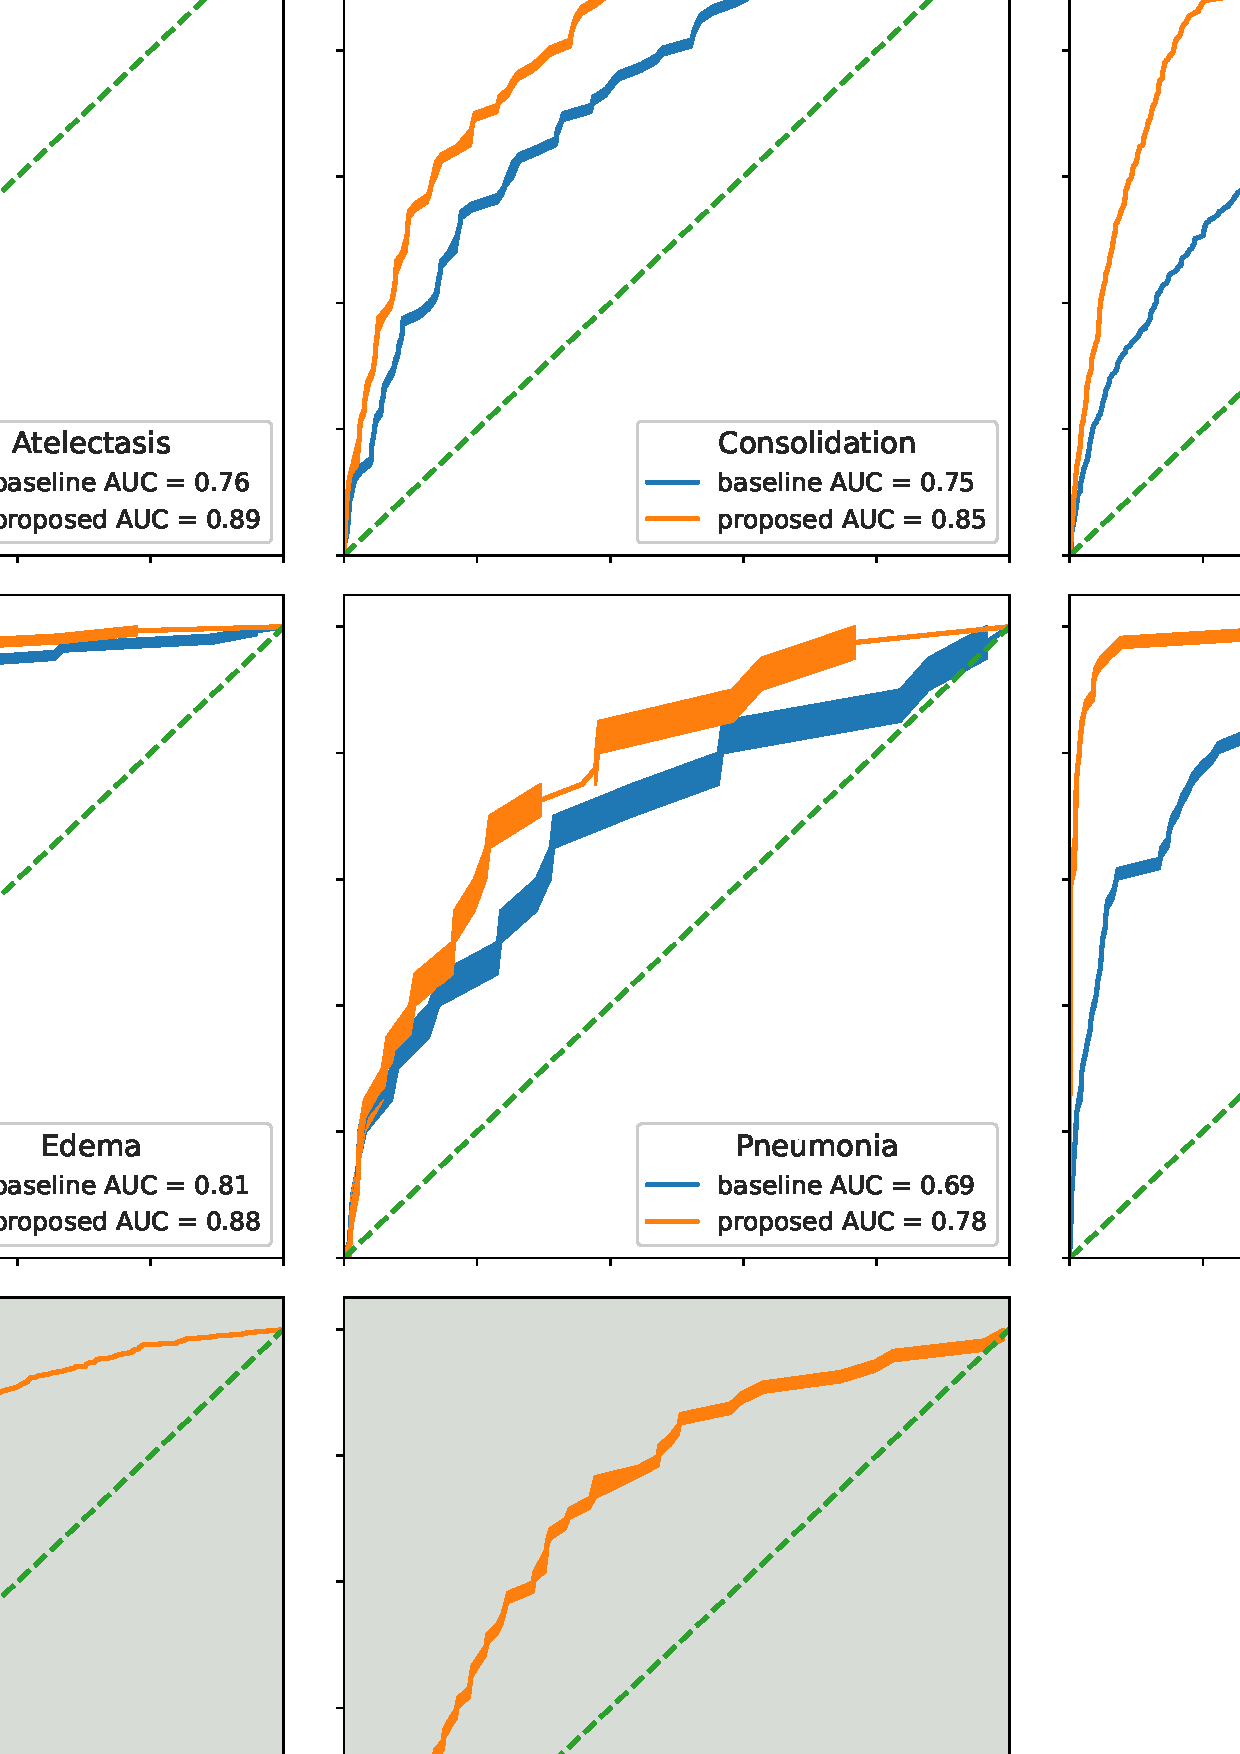
\includegraphics[width=\textwidth]{\figurepath{roc_curve/default_NIH_logit/roc_curve_NIH_logit_default.pdf}}%
    \caption{Comparative analysis of the ROC curves for eight thoracic pathologies using the baseline and the logit based proposed technique. Each subplot illustrates the overlaid ROC curves for both techniques pertaining to a specific pathology. The subplots highlighted with a darker background, represent parent class diseases.}%
    \label{fig:taxonomy.fig.2.roc_curve_nih_logit_default}
\end{figure}

Figure~\ref{fig:taxonomy.fig.2.roc_curve_nih_logit_default} illustrates a comparison between the performance of the baseline technique and the proposed logit-based method (Approach 1 discussed in the Methods section) in detecting eight thoracic pathologies. These eight pathologies include the pathologies with child classes and their respective child classes, as shown in Figure~\ref{fig:taxonomy.fig.1.taxonomy_structure}. The individual subplots exhibit overlaid receiver operating characteristic (ROC) curves, each of which corresponds to a specific pathology. The present analysis employed a model that was derived through the application of the test dataset from the NIH dataset to a pre-trained model. The latter had undergone training on various publicly available thoracic datasets, with the aim of allowing the identification of 18 different pathologies related to the thorax. The last two subplots, showcased with a darker background, showcase the roc curves for parent classes diseases. As these parent class diseases were not influenced by the proposed technique, their ROC curves and corresponding Area Under the Curve (AUC) values remain consistent with the baseline technique. The ROC curve and its corresponding AUC for the six child classes demonstrate a significant improvement for the proposed technique in comparison to the baseline technique.


\begin{figure}[htbp]
    \centering
    \includegraphics[width=\textwidth]{\figurepath{roc_curve/default_NIH_loss/roc_curve_NIH_loss_default.pdf}}
    \caption{Comparative analysis of the ROC curves for eight thoracic pathologies using the baseline and the loss based proposed technique. Each subplot illustrates the overlaid ROC curves for both techniques pertaining to a specific pathology. The subplots highlighted with a darker background, represent parent class diseases.}%
    \label{fig:taxonomy.fig.3.roc_curve_nih_loss_default}%
\end{figure}


Figure~\ref{fig:taxonomy.fig.3.roc_curve_nih_loss_default} illustrates a comparison between the performance of the baseline technique and the proposed loss-based method (Approach 2 discussed in the Methods section) in detecting eight thoracic pathologies. These eight pathologies include two parent classes and their respective child classes, as shown in Figure~\ref{fig:taxonomy.fig.1.taxonomy_structure}. The individual subplots exhibit overlaid ROC curves, each of which corresponds to a specific pathology. The present analysis employed a model that was derived through the application of the test dataset from the NIH dataset to a pre-trained model. The latter had undergone training on various publicly available thoracic datasets, with the aim of allowing the identification of 18 different pathologies related to the thorax. The last two subplots, showcased with a darker background, showcase the roc curves for parent classes diseases. As these parent class diseases were not influenced by the proposed technique, their ROC curves and corresponding AUC values remain consistent with the baseline technique. The ROC curve and its corresponding AUC for the six child classes demonstrate a significant improvement for the proposed technique in comparison to the baseline technique.

\section{Discussion and Conclusion}
The study presented two Hierarchical Multilabel Classification Methods for Enhanced Thoracic Disease Diagnosis in Chest Radiography. One method refered to as ``loss'' udpates the value of loss for pathologies according to their parent pathologies. This method is purticularly useful for both fine-tuning the existing pre-trained models and training from scratch. A second method refered to as ``logit'' is also proposed where the logit values of each pathology is updated based on the logit value of their parent pathologies. This technique is particularly useful when the ground truth labels are not available. This method improves the performance of existing pre-trained models solely based on the taxonomical relationship of pathologies in the model without any need for availablility of ground truth labels.

The results, as indicated in Tables~\ref{tab:taxonomy.table.2.auc_default} and 3, show the F1 score and AUC performance of two methods (``logit'', and ``loss'') with respect to baseline on the CheX, NIH, and PC chest radiograph datasets for various pathologies. Hierarchical multi-label classification approaches demonstrated a significant improvement in the accuracy and efficiency of thoracic disease diagnosis. This was particularly evident in the AUC performance, where the ``loss'' and ``logit'' methods consistently outperformed the ``baseline'' across most pathologies in the CheX, NIH, and PC datasets.

Modifying logits provides a simple yet effective means of incorporating the label hierarchy without substantially changing existing model architectures. However, this approach can obscure the effects of optimization and learning. On the contrary, modifying loss values more directly aligns with the model optimization process and allows fine-tuning of the hierarchical influence through weighting factors. This approach also promotes consistency with established hierarchical relationships and robustness to label noise.

In general, both techniques were effective in using the disease taxonomy to enhance classification performance, indicating the value of leveraging label relationships in medical image classification. The loss-based technique generally showed higher performance gains, suggesting that it may more accurately capture hierarchical dependencies during model training.

The improvement in interpretability offered by these hierarchical techniques can potentially aid clinicians by providing insight into the models' predictions. The ability to explore predictions at different levels of granularity based on taxonomy may facilitate personalized diagnoses based on specific clinical needs.

However, limitations remain. Techniques require predefined label hierarchies, which can be challenging to construct for complex diseases. Further refinement of the hyperparameter tuning procedures may yield even higher performance. Future work could explore the integration of label hierarchies directly into model architectures to achieve end-to-end learning of hierarchical relationships.

In summary, incorporating hierarchical label relationships through modifying either logits or loss functions presents an effective strategy for improving the multi-label classification tasks.

\section*{Appendices}
\section*{Acknowledgements}



\renewcommand{\chapterpath}[1]{Chapters/crowd/#1}
\renewcommand{\figurepath}[1]{\chapterpath{figures}/#1}
% \input{\chapterpath{commands.tex}}

% \chapter{\addtitle}
\chapter{Crowd-Certain: Uncertainty-Based Weighted Soft Majority Voting with Applications in Crowdsourcing and Ensemble Learning}
Accurate diagnosis of thoracic diseases from chest radiographs is a challenging task that can lead to diagnostic errors with negative patient outcomes. In this study, we propose a novel hierarchical multilabel classification technique that incorporates a conditional loss function to improve the identification of common thoracic diseases in chest radiographic images. The proposed method leverages a predefined disease taxonomy to account for interrelationships among diseases, enhancing the classification performance of machine learning models. Our approach can be seamlessly integrated into existing pre-trained models without the need for re-optimization, ensuring efficiency and broad applicability. To evaluate the effectiveness of the proposed technique, experiments were conducted on several diverse and publicly available datasets, including CheXpert, PadChest, and NIH Chest-Xray14. The results demonstrate that the proposed technique significantly improves the precision and interpretability of machine learning models for thoracic disease on chest radiography. This approach has the potential to promote an accurate and efficient diagnosis by providing radiologists with an additional layer of decision support, ultimately leading to better patient outcomes.
}%

\textbf{KEYWORDS:\ } Supervised learning, crowdsourcing, confidence score, soft weighted majority voting, label aggregation, annotator quality, error rate estimation, multi-class classification, ensemble learning, uncertainty measurement
}%

\newpage

\section{Introduction}
Supervised learning techniques require a large amount of labeled data to train models to classify new data~\cite{jiang_wrapper_2019,jiang_class_2019}. Traditionally, data labeling has been assigned to experts in the domain or well-trained annotators~\cite{tian_MaxMargin_2019}. Although this method produces high-quality labels, it is inefficient and costly~\cite{li_noise_2016,li_noise_2019}.  Social networking provides an innovative solution to the labeling problem by allowing data to be labeled by online crowd annotators. This has become feasible, as crowdsourcing services such as Amazon Mechanical Turk (formerly CrowdFlower) have grown in popularity. Crowdsourcing systems have been used to accumulate large amounts of labeled data for applications such as computer vision~\cite{deng_imagenet_2009,liu_Variational_2012} and natural language processing~\cite{karger_Budget_2014}. However, because of individual differences in preferences and cognitive abilities, the quality of labels acquired by a single crowd annotator is typically low, thus jeopardizing applications that rely on these data. This is because crowd annotators are not necessarily domain experts and may lack the necessary training or expertise to produce high-quality labels.
Aggregation after repeated labeling is one method for handling annotators with various abilities. Label aggregation is a process used to infer an aggregated label for a data instance from a multi-label set~\cite{sheshadri_SQUARE_2013}. Several studies have demonstrated the efficacy of repeated labeling~\cite{tu_multilabel_2018,zhang_multilabelinferencecrowdsourcing_2018}. Repeat labeling is a technique in which the same data are labeled by multiple annotators, and the results are combined to estimate an aggregated label using majority voting (MV) or other techniques. In the case of MV, an aggregated label is the label that receives the most votes from the annotators for a given data instance. This can help reduce the impact of biases or inconsistencies made by annotators. Several factors, such as problem-specific characteristics, the quality of the labels created by the annotators, and the amount of data available, can influence the effectiveness of the aggregation methodologies. Consequently, it is difficult to identify a clear winner among the different techniques. For example, in binary labeling, one study~\cite{sheshadri_SQUARE_2013} discovered that Raykar's~\cite{raykar_Learning_2010} technique outperformed other aggregation techniques. However, according to another study~\cite{zheng_Truth_2017}, the traditional Dawid-Skene (DS) model~\cite{dawid_Maximum_1979} was more reliable in multi-class settings (where data instances can be labeled as belonging to multiple classes).
Furthermore, regardless of the aggregation technique used, the performance of many aggregation techniques in real-world datasets remains unsatisfactory~\cite{liu_Exploiting_2021}. This can be attributed to the complexity of these datasets, which often do not align with the assumptions and limitations of different methods. For example, real-world datasets may present issues such as labeling inaccuracies, class imbalances, or overwhelming sizes that challenge efficient processing with available resources. These factors can adversely affect the effectiveness of label aggregation techniques, potentially yielding less than optimal results for real-world datasets.
Prior information may be used to enhance the label aggregation procedure.
This can include domain knowledge, the use of quality control measures and techniques that account for the unique characteristics of annotators and data. Knowing the reliability of certain annotators, it is possible to draw more accurate conclusions about labels~\cite{li_Crowdsourced_2017}. For instance, in the label aggregation process, labels produced by more reliable annotators (such as domain experts) may be given greater weight. The results of the label aggregation process can also be validated using expert input~\cite{liu_Improving_2017}. During the labeling process, domain experts can provide valuable guidance and oversight to ensure that the labels produced are accurate and consistent.
The agnostic requirement for general-purpose label aggregation is that label aggregation cannot use information outside the labels themselves. This requirement is not satisfied in most label aggregation techniques~\cite{zhang_Crowdsourced_2019}. The agnostic requirement ensures that the label aggregation technique is as general as possible and applicable to a wide range of domains with minimal or no additional context.
The uncertainty of annotators during labeling can provide valuable prior knowledge to determine the appropriate amount of confidence to grant each annotator while still adhering to the requirement of a general-purpose label aggregation technique. We developed a method for estimating the reliability of different annotators based on the annotator's own consistency during labeling. We take this concept a step further by calculating a weight for each annotator based not only on their own reliability but also on the reliability scores of all other workers involved. This consideration of inter-reliability ensures a more comprehensive and dynamic weighting process, adjusting to the overall performance of the entire group of annotators. Thus, the generated weights become a robust measure of both individual and collective trustworthiness, which significantly improves the accuracy and efficacy of our labeling aggregation method.
We propose a novel method called ``crowd-certain'', which provides a more accurate aggregation of labels, ultimately leading to improved overall performance in both crowdsourcing and ensemble learning scenarios. The proposed method uses the consistency of annotators versus a trained classifier to determine their reliability. The experimental results conducted on multiple crowdsourcing datasets show that the proposed technique generates a reliability score that closely follows  a set of reference values representing the annotator's degree of reliability and outperforms prior methods (Gold Majority Vote, MV, MMSR, Wawa, Zero-Based Skill, GLAD, and Dawid Skene), in terms of accuracy, particularly when few annotators are available.
The remainder of this paper is organized as follows. Section~\ref{sec:crowd.relatedwork} examines related work involving label aggregation algorithms. In Section~\ref{sec:crowd.method}, we provide a detailed explanation of our proposed technique. Section\ref{sec:crowd.results} presents the experiments and findings. Finally, Section~\ref{sec:crowd.discussion} summarizes the findings and identifies the main directions for future research.

\section{Related Work}\label{sec:crowd.relatedwork}
Numerous label aggregation algorithms have been developed to capture the complexity of crowdsourced labeling systems, including techniques based on annotator reliability~\cite{bi_Learning_2014,demartini_Zencrowd_2012}, confusion matrices~\cite{raykar_Learning_2010,zhang_Spectral_2014}, intentions~\cite{bi_Learning_2014,kurve_MultiCategory_2015}, biases~\cite{zhang_Imbalanced_2013,hernandez-gonzalez_Note_2019, welinder_Multidimensional_2010}, and correlations~\cite{ma_Gradient_2020}. However, because crowdsourced labeling is inherently dynamic and uncertain, developing a technique that can work in most situations is extremely challenging. Many techniques~\cite{liu_Variational_2012,karger_Budget_2014,raykar_Learning_2010,dalvi_Aggregating_2013,ghosh_Who_2011} utilize the Dawid and Skene (DS) generative model~\cite{dawid_Maximum_1979}. Ghosh~\cite{ghosh_Who_2011} extended the DS model by using singular value decomposition (SVD) to calculate the reliability of the annotator. Similarly to Ghosh~\cite{ghosh_Who_2011}, Dalvi~\cite{dalvi_Aggregating_2013} used SVD to estimate true labels with a focus on the sparsity of the labeling matrix. In crowdsourcing, it is common for the labeling matrix to be sparse, meaning that not all annotators have labeled all the data. This may be due to several factors, such as the cost of labeling all data instances or the annotators' time constraints. Karger~\cite{karger_Budget_2014} described an iterative strategy for binary labeling based on a one-coin model~\cite{ghosh_Who_2011}. Karger~\cite{karger_Budget_2014} extends the one-coin model to multi-class labeling by converting the problem into $k-1 $ binary problems (solved iteratively), where $k $ is the number of classes.
The MV technique assumes that all annotators are equally reliable. For segmentation, Warfield~\cite{warfield_Simultaneous_2004} proposed simultaneous truth and performance level estimation (STAPLE), a label fusion method based on expectation maximization. STAPLE ``weighs'' expert opinions during label aggregation by modeling their reliability. Since then, many variants of this technique have been proposed~\cite{winzeck_ISLES_2018,commowick_Objective_2018,asman_Robust_2011,asman_Formulating_2012, eugenioiglesias_Unified_2013, jorgecardoso_STEPS_2013,asman_NonLocal_2013,akhondi-asl_Logarithmic_2014}. The problem with these label aggregation approaches is that they require the computation of a unique set of weights for each sample, necessitating the re-evaluation of the annotators' weights when a new instance is added.
Among the numerous existing label aggregation strategies, MV remains the most efficient and widely used approach~\cite{tao_Label_2020}. If we assume that all annotators are equally reliable and that their errors are independent of one another, then, according to the theory of large numbers, the likelihood that the MV is accurate increases as the number of annotators increases. However, the assumption that all annotators are equally competent and independent may not always hold. Furthermore, MV does not provide any additional information on the degree of disagreement among the annotators (As an example, consider the scenario where four of seven doctors think patient A needs immediate surgery, while all seven think patient B needs immediate surgery; MV will simply label ``yes'' in both cases).
To address this problem, additional measures such as inter-annotator agreement (IAA) have been used~\cite{artstein_InterAnnotator_2017}. IAA is a measurement of the agreement among multiple annotators who label the same data instance. Typically, IAA is calculated using statistical measures, such as Cohen's kappa, Fleiss's kappa, or Krippendorff's alpha~\cite{krippendorff_Content_2018}. These measures consider both the observed agreement between the annotators and the expected agreement owing to random chance. IAA can also be visualized using a confusion matrix or annotation heatmap, which illustrates the distribution of labels assigned by the annotators. This can help identify instances where the annotators disagree or are uncertain and can guide further analysis to improve the annotation~\cite{carletta_Assessing_1996}.
Recently, Sheng~\cite{sheng_Majority_2019} proposed a technique that provided a confidence score along with an aggregated label. The main problem with this approach is that it assumes that all annotators are equally capable when calculating the confidence score. Tao~\cite{tao_Label_2020} improved Sheng's approach by assigning different weights to annotators for each instance. This weighting method combines the specific quality $s_\alpha^{(i,k)} $ for the annotator $\alpha $ and instance $i $ and the overall quality $\tau_\alpha$ across all instances. Inspired by Li's technique~\cite{li_Incorporating_2018}, Tao evaluates the similarity between the annotator labels for each instance. To derive the specific quality $s_{\alpha}^{(i)}$, Tao counts the number of annotators who assigned the same label as the annotator $\alpha $ for that instance. To calculate the overall quality $\tau_\alpha $, Tao performs a 10-fold cross-validation to train each of the 10 classifiers on a different subset of data using the labels provided by the annotator $\alpha $ as true labels and then assigns the average accuracy across all remaining instances as $\tau_\alpha $. The final weight for annotator $\alpha $ and instance $i $ is then calculated using the sigmoid function $\gamma_{i,\alpha}=\tau_\alpha\left(1+{\left(s_{\alpha}^{(i)}\right)}^{2}\right) $. However, Tao's technique~\cite{tao_Label_2020} has some drawbacks. It relies on the labels of other annotators to estimate $s_{\alpha}^{(i)} $. However, different annotators have varying levels of competence (reliability) when labeling the data, and therefore, relying on their labels to measure $s_{\alpha}^{(i)} $ will result in propagating the errors and biases of their labels during weight estimation. Furthermore, Tao's technique~\cite{tao_Label_2020} relies on the labels provided by each annotator $\alpha $ to estimate their respective $\tau_\alpha $ by assuming that the trained classifiers can learn the inherent characteristics of the datasets even in the absence of ground truth labels. While that may be true in some cases, it typically leads to suboptimal measurement and the propagation of biases and errors, from both the annotator's labels and the classifier, into weight estimation.
\section{Methods}\label{sec:crowd.method}
We propose a novel method called ``crowd-certain'' which focuses on leveraging uncertainty measurements to improve decision-making in crowdsourcing and ensemble learning scenarios. Crowd-Certain employs a weighted soft majority voting approach, where the weights are determined based on the uncertainty associated with each annotator's labels. Initially, we use uncertainty measurement techniques to calculate the degree of consistency of each annotator during labeling. Furthermore, to ensure that the proposed technique does not calculate a high weight for annotators who are consistently wrong (for example, when a specific annotator always mislabels a specific class, and hence demonstrates a high consistency while having low accuracy), we extend the proposed technique by penalizing the annotators for instances in which they disagree with the aggregated label obtained using MV\@. To mitigate the reliance on training a classifier on an annotator's labels, which may be inaccurate, we train an ensemble of classifiers for each annotator. In addition, we report two confidence scores along with the aggregated label to provide additional context for each calculated aggregate label. We report a single weight for all instances in the dataset. As will be demonstrated in Section~\ref{sec:crowd.results}, the proposed crowd-certain method is not only comparable to other techniques in terms of accuracy for scenarios with a large number of annotators, but also provides a significant improvement in accuracy for scenarios where the number of annotators may be limited. Furthermore, by assigning a single weight to each annotator for all instances in the dataset, the model can assign labels to new test instances without recalculating the annotator weights. This is especially advantageous in situations where annotators are scarce as it enables the model to make accurate predictions with minimal dependence on the annotator input. This characteristic of the crowd-certain method can significantly reduce the time and resources required for labeling in practical applications. When deploying the model in real-world scenarios such as medical diagnosis, fraud detection, or sentiment analysis, it could be advantageous to be able to assign labels to new instances without constantly recalculating annotator weights.
\subsection{Glossary of Symbols}
For convenience, the following list summarizes the major symbols used in the subsequent discussion:
\begin{itemize}[itemsep=1em]
\renewcommand{\textbullet}{}
    \item  $N$: Number of instances.
    \item  $M$: Number of annotators.
    \item  $y^{(i,k)} \in \{0,1\} $: True label for the $k $-th class for instance $i $.
    \item  $z_\alpha^{(i,k)} \in \{0,1\} $: Label given by annotator $\alpha $ for $k $-th class for instance $i $.
    \item  ${{\underset\alpha{\mathrm{MV}}}{\left(z_\alpha^{(i,k)}\right)}} $: Majority voting technique (the label that receives the most votes) applied to annotator labels for class $k $ and instance $i $.
    \item  $\pi_\alpha^{(k)} $: Probability threshold used as reference value representing the annotator's degree of reliability. It is used to generate sample binary labels (fictitious ground truth label set) for annotator $\alpha $ for class $k $. For example, the threshold values may be obtained from a uniform distribution in the interval $0.4 $ to $1 $, i.e., $\pi_\alpha^{(k)} \sim U(0.4,1) $.
    \item  $X^{(i)} $: Data for instance $i$.
    \item  $Y^{(i)}=\left\{y^{(i,1)},y^{(i,2)},\;\dots,y^{(i,K)}\right\} $: True label set, for instance $i $. For example, consider a dataset that is labeled for the presence of cats, dogs, and rabbits in any given instance. If a given instance $X^{(i)} $ has cats and dogs but not rabbits, then $Y^{(i)}=\{1,1,0\} $.
    \item  $Z_{\alpha}^{(i)}=\left\{z_\alpha^{(i,1)}, z_\alpha^{(i,2)}, \dots, z_\alpha^{(i,K)}\right\} $: Label set given by the annotator $\alpha $ for instance $i $.
    \item $K$: number of categories (aka classes) in a multi-class multi-label problem. For example, if we have a dataset labeled for the presence of cats, dogs, and rabbits in any given instance, then $K=3$.
    \item  $\rho^{(i)}$: Randomly generated number  between 0 and 1 for instance $i $. It is obtained from a uniform distribution, i.e., $\rho^{(i)} \sim U(0,1) $ This number is used to determine, for each instance $i$, whether the true label should be assigned to each fictitious annotator's label. For each class $k$, if the annotator's probability threshold $\pi_\alpha^{(k)}$ is greater than $\rho^{(i)}$, the true label $y^{(i,k)}$ is assigned; otherwise, an incorrect label $1 - y^{(i,k)}$  is assigned.
    \item  $\Pi_\alpha=\left\{ \pi_\alpha^{(1)} , \pi_\alpha^{(2)}  , \dots, \pi_\alpha^{(K)} \right\} $: set of $K $ probability thresholds for annotator $\alpha $.
    \item  $\mathbb{X}=\left\{X^{(i)}\right\}_{i=1}^{N} $: Set of all instances.
    \item  $\mathbb{Y}=\left\{Y^{(i)}\right\}_{i=1}^{N} $: Set of all true labels.
    \item  $\mathbb{Z}_\alpha=\left\{Z_\alpha^{(i)}\right\}_{i=1}^{N} $: Set of all labels for the annotator $\alpha $.
    \item  $\widehat{\mathbb{Y}}= \left\{\widehat{Y}^{(i)}\right\}_{i=1}^{N} $: Set of all aggregated labels.
    \item  $\mathbb{P}=\left\{\rho^{(i)}\right\}_{i=1}^{N} $: Set of $N $ randomly generated numbers .
    \item  $\mathbb{D}=\left\{\mathbb{X},\mathbb{Y}\right\} $: Dataset containing all instances and all true labels.
    \item  $\mathbb{D}_\alpha=\left\{\mathbb{X},\mathbb{Z}_\alpha\right\} $: Dataset containing the labels given by the annotator $\alpha $.
    \item  $\mathbb{D}_\alpha^\text{train}$, $\mathbb{D}_\alpha^{\text{test}} $: Train and test crowd datasets randomly selected from $\mathbb{D}_{\alpha} $ where $\mathbb{D}_\alpha^{\text{train}} U \mathbb{D}_\alpha^{\text{test}} = \mathbb{D}_\alpha $ and $\mathbb{D}_\alpha^{\text{train}} \bigcap \mathbb{D}_{\alpha}^{\text{test}}=\varnothing $
    \item  $f_{\alpha}^{(g)}(\cdot)$: Classifier $g $ trained on dataset $\mathbb{D}_{\alpha}^{\mathrm{train}} $ with random seed number $g $ (which is also the classifier index)
    \item  $P_{\alpha}^{(i),(g)} = \left\{ p_{\alpha}^{(i,k),(g)} \right\}_{k=1}^{K} $: Predicted probability set obtained in the output of the classifier $f_{\alpha}^{(g)}(\cdot) $ representing the probability that each class $k $ is present in the sample.
    \item  $\theta_{\alpha}^{(k),(g)} $: Binarization threshold. To obtain this, we can utilize any existing thresholding technique. For example, in one technique, we analyze the ROC curve and find the corresponding threshold where the difference between the true positive rate (sensitivity) and false positive rate (1-specificity) is maximum. Alternatively, we could simply use $0.5 $.
    \item  $t_\alpha^{(i,k),(g)} =
        \begin{cases}
            1 & \text{if } p_\alpha^{(i,k),(g)} \geq \theta_\alpha^{(k),(g)}, \\
            0 & \text{otherwise}.
        \end{cases} $: Predicted label obtained by binarizing $p_\alpha^{(i,k),(g)} $.
    \item  $\eta_{\alpha}^{(i,k)} = {{\underset g{\mathrm{MV}}}{ \left(t_\alpha^{(i,k),(g)}\right) }} $: The output of the majority vote applied to the predicted labels obtained by the $G $ classifiers.
    \item  $\Delta_{\alpha}^{(i,k)} $: Uncertainty score.
    \item  $c_\alpha^{(i,k)} $: Consistency score.
    \item  $\omega_\alpha^{(k)} $: Estimated weight for annotator $\alpha $ and class $k $.
    \item  $\nu^{(i,k)} = \frac{1}{{M}}{\sum_{\alpha}{\omega_\alpha^{(k)} \; \eta_\alpha^{(i,k)}}} $ : Final aggregated label for class $k $ and instance $i $.
\end{itemize}
\subsection{Risk Calculation}
Label aggregation is frequently used in various machine learning tasks, such as classification and regression, when multiple annotators assign labels to the same data points. The aggregation model refers to the underlying function that maps a set of multiple labels, obtained by different annotators, into one aggregated label. In the context of label aggregation, this model can be a neural network, a decision tree, or any other machine learning algorithm capable of learning to aggregate labels provided by multiple annotators. The objective of this study is to develop an aggregation model capable of accurately determining true labels despite potential disagreements among annotators. One common method to achieve this involves minimizing the total error (or disagreement) between the annotators' assigned labels and the true labels, as follows:
\begin{equation}
E = \sum_{i=1}^N \sum_{a=1}^M \left( \sum_{k=1}^K \delta\left(y^{(i,k)}, z_\alpha^{(i,k)}\right) \right)
\label{eq:crowd.Eq.1.risk.error}
\end{equation}
where $\delta $ is the Kronecker delta function.
Although error is a crucial aspect in determining the aggregation model's performance, it treats false positives and false negatives with equal weight. However, in many practical scenarios, it is essential to weigh false positives and false negatives differently depending on the specific context and potential consequences of each type of misclassification. The concept of risk allows us to achieve this by incorporating a loss function, which assigns different weights to different types of errors. In this way, risk serves as a weighted calculation of error, enabling us to better evaluate the performance of an aggregation model and its generalization capability.
Let us denote loss function, $\mathcal{L}(\cdot)$, as a function that quantifies the discrepancy between the predicted labels and the true labels, accounting for the varying importance of different types of errors.
Risk, denoted as $R(h) $, represents the expected value of a loss function over all possible data instances.  In practice, our goal is to minimize the risk to achieve optimal performance on unseen data. However, since we only have access to a limited dataset (empirical distribution), we instead work with the empirical risk. This limitation may arise because of the need to reserve a portion of our data for testing and validation or because no dataset can fully capture all possible data instances in the real world. However, minimizing risk alone could result in overfitting, in which the aggregation model learns the noise in the training data rather than the underlying patterns, resulting in poor generalization to unseen data. To improve generalizability, it is necessary to employ regularization techniques to strike a balance between the complexity of the aggregation model and its ability to fit the training data.
Risk measurement enables us to assess the aggregation model's performance in terms of accuracy, overfitting (when risk is minimized but the model performs poorly on unseen data), and model complexity.
Assume that the aggregation model $h (\cdot) $ is a function that takes a set of $M $ label sets $Z^{(i)} $ for each instance $i $ in the training data and calculates an aggregated label set $\widehat{Y}^{(i)} $ as an estimate of the true label set $Y^{(i)} $. Our goal is to find an aggregation model $h(\cdot) $ that minimizes risk defined as follows:
\begin{equation}
R(h) = \frac{1}{N} \sum_{i=1}^{N} \mathcal{L} \left( Y^{(i)}, h\left(\left\{Z_{\alpha}^{(i)}\right\}_{\alpha=1}^{M}\right)\right)
\label{eq:crowd.Eq.2.risk.emp}
\end{equation}
In this context, $\mathcal{L}(\cdot) $ represents an arbitrary loss function, which quantifies the discrepancy between predicted labels and true labels while accounting for the varying importance of different types of errors.
Our goal is to choose an aggregation model $\widehat{h} $ that minimizes the risk, following the principle of risk minimization~\cite{vapnik_Principles_1991}:
\begin{equation}
\widehat{h} = \underset{h}{\text{argmin}}  R(h)
\label{eq:crowd.Eq.3.risk.h}
\end{equation}

\subsection{Generating Annotators’  Label Sets from Ground Truth}
In order to evaluate the proposed crowd-certain technique (with and without penalization) as well as other aggregation techniques, we create $M$ fictitious annotators. To synthesize a multi-annotator dataset from a dataset with existing ground truth, we use a uniform distribution in the interval from $0.4 $ to $1 $, i.e., $\pi_\alpha^{(k)} \sim U\left(0.4,1\right) $ (however other ranges can also be used) to obtain $M \times  K$ probability thresholds $\Pi $, where $K$ is the number of classes. (Note that
an annotator may be skilled at labeling dogs, but not rabbits.) Then we use these probability thresholds to generate the crowd label set $Z_{\alpha}^{(i)} $ from the ground truth labels for each instance $i $.
For each annotator $\alpha $, each instance $i $ and class $k $ in the dataset is assigned its true label with probability $\pi_\alpha^{(k)}$ and the opposite label with probability $ (1-\pi_\alpha^{(k)})$. To generate the labels for each annotator $\alpha $, a random number $0 < \rho^{(i)} < 1 $ is generated for each instance $i $ in the dataset. Then $\forall \alpha,k \; \; \text{if} \; \; \rho^{(i)}\leq \pi_\alpha^{(k)}$. Then the true label is used for that instance and class for the annotator $\alpha $; otherwise, the incorrect label is used.
The calculated annotator labels $z_{\alpha}^{(i,k)} $ for each annotator $\alpha $, instance $i $ and class $k $ are as follows:
\begin{equation}
    z_{\alpha}^{(i,k)} =
    \begin{cases}
        y^{(i,k)} & \text{if } \rho^{(i)}  \leq \pi_\alpha^{(k)} , \\
        1 - y^{(i,k)} & \text{if } \rho^{(i)} > \pi_\alpha^{(k)} ,
    \end{cases} \quad \forall i, a, k
    \label{eq:crowd.Eq.4.fictitious_label}
\end{equation}
To evaluate the proposed techniques over all data instances, a k-fold cross-validation is employed.

\subsection{Uncertainty Measurement}\label{subsec:crowd.uncertainty}
A common approach to measure uncertainty is to increase the number of data instances $X $ in the test dataset $\mathbb{D}_\alpha^{\mathrm{test}} $ to create multiple variations of each sample data $X^{(i)} $~\cite{ayhan_TestTime_2018}. In this approach, for each instance $i $, we apply randomly generated spatial transformations and additive noise to the input data $X^{(i)} $ to obtain a transformed sample and repeat this process $G $ times to obtain a set of $G $ transformed samples.
However, this approach is mostly suitable for cases where the input data comprises images or volume slices. Since the datasets used in this study consist of feature vectors instead of images or volume slices, this approach cannot be used. To address this problem, we introduced a modified uncertainty measurement approach, in which instead of augmenting the data instances $X^{(i)} $, we feed the same sample data to different classifiers.
For the choice of classifier, we can either use a probability-based classifier such as random forest and train it under $G $ different random states or train various classifiers and address the problem in a manner similar to ensemble learning (using a set of $G $ different classification techniques such as random forest, SVM, CNN, Adaboost, etc.). In either case, we obtain a set of $G $ classifiers ${\left\{f_{\alpha}^{(g)}( \cdot)\right\}}_{g=1}^G $ for each annotator $\alpha $. The classifier $f_{\alpha}^{(g)}( \cdot) $ is a pre-trained or pre-designed model that has been trained on a labeled training dataset $\mathbb{D}_\alpha^{\mathrm{train}} $. This training process enables $f_{\alpha}^{(g)}(\cdot) $ to learn the underlying patterns in the data and make predictions on unseen instances.
After training, we feed the test samples $X^{(i)}\in \mathbb{X}^{\text{test}} $ to the $g $-th classifier $f_{\alpha}^{(g)}(\cdot) $ as test cases. The classifier $f_{\alpha}^{(g)}(\cdot) $ then outputs a set of predicted probabilities $\left\{p_{\alpha}^{(i,k),(g)}\right\}_{k=1}^{K} $ representing the probability that class $k $ is present in the sample. Consequently, we obtain a collection of $G $ predicted probability sets $\left\{ \left\{ p_{\alpha}^{(i,k),(g)}\right\}_{k=1}^K \right\}_{g=1}^G $ for each annotator $\alpha $ and instance $i $. The set $\left\{p_{\alpha}^{(i,k),(g)}\right\}_{g=1}^G $ contains the predicted probabilities for class $k $, annotator $\alpha $, and instance $i $. Disagreements between predicted probabilities $\left\{p_{\alpha}^{(i,k),(g)}\right\}_{g=1}^G $ can be used to estimate uncertainty.
The reason for using classifiers rather than using the crowdsourced labels directly is two-fold. Using a probabilistic classifier helps us calculate uncertainty based on each annotator's labeling patterns that the classifier learns. Furthermore, this approach provides us with a set of pre-trained classifiers $\left\{ \left\{f_{\alpha}^{(g)}(\cdot) \right\}_{g=1}^G  \right\}_{a=1}^{M} $ that can be readily utilized on any new data instances without the need for those samples to be labeled by the original annotators.
The index value $g  \in \{1,2,\dots,G\} $ is used as the random seed value during training of the $g$\-th classifier for all annotators.
Define $t_{\alpha}^{(i,k),(g)} $ as the predicted label obtained by binarizing the predicted probabilities $p_{\alpha}^{ (i,k),(g)} $ using the threshold $\theta_{\alpha}^{(k),(g)} $ as shown in the Glossary of Symbols section.
Uncertainty measures are used to quantify the level of uncertainty or confidence associated with the predictions of a model. In this work, we need to measure the uncertainty $u_{\alpha}^{(i,k)}$ associated with the model predictions. Some common uncertainty measurement measures are as follows.

\subsubsection{Entropy}
Entropy is a widely used measure of uncertainty in classification problems. In an ensemble of classifiers, entropy serves as a quantitative measure of the uncertainty or disorder present in the probability distribution of the predicted class labels. A higher entropy value indicates a greater degree of uncertainty in the predictions, as the predictions of the individual classifiers in the ensemble are significantly different. In contrast, a lower entropy value indicates reduced uncertainty as the ensemble assigns very similar probabilities to a particular class, indicating strong agreement among the classifiers and increased confidence in their collective prediction. The formula for calculating entropy is as follows:
\begin{equation}
\Delta_{\alpha}^{(i,k)}=H\left(\left\{p_{\alpha}^{(i,k),(g)}\right\}_{g=1}^{G}\right)=-\sum_{g}{p_{\alpha}^{(i,k),(g)} \log\left(p_{\alpha}^{(i,k),(g)}\right)}
\label{eq:crowd.Eq.5.uncertainty}
\end{equation}

\subsubsection{Standard Deviation}
In regression problems, standard deviation is often used to quantify uncertainty. It measures the dispersion of predicted values around the mean. A greater standard deviation indicates greater uncertainty of the prediction. For a set of predicted values $ \{t_{\alpha}^{(i,k),(g)} \}_{g=1}^G $ with mean value $\mu $, the standard deviation is defined as.
\begin{equation}
   \Delta_{\alpha}^{(i,k)}=\text{SD}\left(\left\{t_{\alpha}^{(i,k),(g)}\right\}_{g=1}^G\right)=\sqrt {\frac{1}{G-1 }\sum_{g=1}^G\left(t_{\alpha}^{(i,k),(g)}-\mu\right)^{2}},\quad\mu=\frac{1}{G}\sum_{g=1}^{G}{t_{\alpha}^{(i,k),(g)}}
    \label{eq:crowd.Eq.6.uncertainty.sd}
\end{equation}

\paragraph{Predictive Interval}
A predictive interval provides a range within which a future observation is likely to fall with a certain level of confidence. For example, a 95\% predictive interval indicates that there is a 95\% likelihood that the true value falls within that range. A greater uncertainty corresponds to wider intervals. In the context of multiple classifiers, the predictive intervals can be calculated by considering the quantiles of the classifier output. For a predefined confidence level $\gamma $ (e.g., 95\%), for a specific class $k $, we need to find the quantiles $Q_{L}^{k} $ and $Q_{U}^{k} $ of the probability distribution of class $k $ predicted by the $G $ classifiers. The uncertainty can be represented by the width of the predictive interval:
\begin{equation}
    \begin{aligned}
        P\left(Q_L^{k} \leq p_{\alpha}^{(i,k),(g)} \leq Q_U^{k}\right) = \gamma
        \\
        \Delta_{\alpha}^{(i,k)} = Q_L^{k} - Q_U^{k}
    \end{aligned}
    \label{eq:crowd.Eq.uncertainty}
\end{equation}
The steps to calculate the predictive interval are as follows:
\begin{enumerate}
    \item Collect the class $k $ probabilities predicted by all $G$ classifiers for a given instance. Then sort the values in ascending order. Let us call this set $P_{\alpha}^{(i,k)}=\mathrm{sorted}\left(\left\{p_{\alpha}^{(i,k),(g)}\right\}_{g=1}^G\right),\quad\forall \alpha,k,i $.
    \item Calculate the lower and upper quantile indices based on the chosen confidence level $\gamma $. The lower quantile index is $L=\mathrm{ceil}\left(\frac{G}{2}\left(1-\gamma\right)\right) $, and the upper quantile index is $U=\mathrm{floor}\left(\frac{G}{2} (1+\gamma)\right) $, where ceil and floor are the ceiling and floor functions, respectively.
    \item Find the values corresponding to the lower and upper quantile indices in the sorted $P_{\alpha}^{(i,k)} $. These values are the lower and upper quantiles $Q_L^{k} $ and $Q_U^{k} $.
    \item Now we have the predictive interval $P\left(Q_L^{k}<=p_{\alpha}^{(i,k),(g)}<=Q_U^{k}\right)=\gamma $, where $Q_L^{k} $ and $Q_U^{k} $ represent the bounds of the interval containing the $\alpha$ proportion of the probability mass.
\end{enumerate}
\subsubsection{Monte Carlo Dropout}
The Monte Carlo dropout~\cite{gal_Dropout_2016a} can be used to estimate uncertainty in neural networks by applying the dropout at test time. Multiple forward passes with dropout generate a distribution of predictions from which uncertainty can be derived using any of the aforementioned techniques (standard deviation, entropy, etc.).
\subsubsection{Bayesian Approaches}
Bayesian methods offer a probabilistic framework to estimate the parameters of the model and make predictions. These methods explicitly model uncertainty by considering prior beliefs about the model parameters and then updating those beliefs based on the observed data. In Bayesian modeling, the model parameters are treated as random variables and a posterior distribution is estimated using these parameters. The following are two common Bayesian approaches for measuring the uncertainty in classification problems.
\begin{itemize}
    \item \relax \textbf{Bayesian model averaging (BMA):} BMA accounts for model uncertainty by combining the predictions of various models using their posterior probabilities as weighting factors. Instead of selecting a single ``best'' model, BMA acknowledges the possibility of multiple plausible models, each with its own strengths and weaknesses~\cite{hoeting_Bayesian_1999}. The steps to implement BMA are as follows. Select a set of candidate models that represent different hypotheses regarding the data-generating process underlying the data. These models may be of various types, such as linear regression, decision trees, neural networks, or any other model suited to the specific problem at hand. Using the available data, train each candidate model. Calculate the posterior probabilities of the models. Using the posterior probabilities of each model as weights, calculate the weighted average of each model's predictions. The weighted average is the BMA prediction for the input instance and class.
    \item \relax \textbf{Bayesian neural networks (BNNs):} BNNs~\cite{mullachery_Bayesian_2018} are an extension of conventional neural networks in which the weights and biases of the network are treated as random variables. The primary distinction between BNNs and conventional neural networks is that BNNs model uncertainty directly in the weights and biases. The posterior distributions of the network weights and biases (learned during training) capture the uncertainty, which can then be utilized to generate predictive distributions for each class. This enables multiple predictions to be generated by sampling these predictive distributions, which can be used to quantify the uncertainty associated with each class.
\end{itemize}
\subsubsection{Committee-Based Methods}
The committee-based method~\cite{wang_Wisdom_2020} involves training multiple models (a committee) and aggregating their predictions. The disagreement between committee members' predictions can be used as a measure of uncertainty. Examples include bagging and boosting ensemble methods and models, such as random forests.
\begin{equation}
    \Delta_{\alpha}^{(i,k)} = \mathrm{VarCommittee}\left(P_{\alpha}^{(i,k)}\right) = \frac{1}{G-1}\sum_{g=1}^G \left(p_{\alpha}^{(i,k),(g)}-\mu\right)^{2},\quad\mu= \frac{1}{G} \sum_{g=1}^G p_{\alpha}^{(i,k),(g)}
    \label{eq:crowd.Eq.8.uncertainty.committee_based}
\end{equation}
\subsubsection{Conformal Prediction}
Conformal prediction~\cite{angelopoulos_Gentle_2021} is a method of constructing prediction regions that maintain a predefined level of confidence. These regions can be used to quantify the uncertainty associated with the prediction of a model.
Steps  to calculate the nonconformity score:
\begin{enumerate}
    \item For each classifier $g $ and each class $k $, calculate the nonconformity score. Here, $\mathrm{score\_function}$ measures the conformity of the prediction with the true label. In the context of this study, the true label can be replaced by $\eta_{\alpha}^{(i,k)} $. A common choice for $\mathrm{score\_function}$ is the absolute difference between the predicted probability and the true label, but other options can be used depending on the specific problem and requirements. Define the nonconformity score as $ \zeta_{k}^{g} = \mathrm{score\_function} \left(p_{\alpha}^{(i,k),(g)}, y^{(i,k)}\right) $
    \item Calculate the p-value $\mathrm{pv}^{(k)} $ for each class $k $ as the proportion of classifiers with nonconformity scores greater than or equal to a predefined threshold $\text{T}^{(k)}: \text{p-values}(k) = \frac{ \left\vert \{g: \;\zeta^{(k),(g)} \geq \text{T}^{(k)} \} \right\vert} {G} $
    \item The p-values calculated for each class $k $ represent the uncertainty associated with that class. A higher p-value indicates a higher level of agreement among the classifiers for a given class, whereas a lower p-value suggests greater uncertainty or disagreement.
\end{enumerate}
The uncertainty measures discussed above are only some of the available options. Selecting an appropriate measure depends on factors such as the problem domain, the chosen model, and the specific requirements of a given application. For this study, we use the variance technique shown in Equation~(\ref{eq:crowd.Eq.6.uncertainty.sd}) as our uncertainty measurement due to its simplicity. However, other measures could also be employed as suitable alternatives.
\subsection{Crowd-Certain: Uncertainty-Based Weighted Soft Majority Voting}
\subsubsection{Consistency Measurement}
Define $c_{\alpha}^{(i,k)} $ as the consistency score for annotator $\alpha $, class $k $ and instance $i $. We calculate this consistency score using the uncertainty score $\Delta_{\alpha}^{(i,k)} $ explained in the previous section. We use two approaches to calculate $c_{\alpha}^{(i,k)} $ from $\Delta_{\alpha}^{(i,k)} $.
\begin{enumerate}
    \item The first approach is to simply subtract the uncertainty from $1 $ as follows:
    \begin{equation}
        c_{\alpha}^{(i,k)}=1-\Delta_{\alpha}^{(i,k)}\;\;,\;\forall i,\alpha,k
        \label{eq:crowd.Eq.9.consistency}
    \end{equation}
    \item In a second approach (shown in Equation~(\ref{eq:crowd.eq.10.consistency-penalized})), we penalize annotators for instances in which their predicted label $\eta_{\alpha}^{(i,k)} $ (explained in the Glossary of Symbols section) does not match the MV of all annotator labels ${{\underset \alpha{\mathrm{MV}}}{\left(z_{\alpha,\;k}^{(i,k)}\right)}} $. As previously discussed, instead of directly working with the annotator's labels $z_{\alpha}^{(i,k)} $, we use the predicted labels obtained from the ensemble of classifiers $\eta_{\alpha}^{(i,k)} $. This methodology does not require repeating the crowd-labeling process for new data samples. In particular, we are likely not to have access to the same crowd of annotators employed in the training dataset.
    \begin{equation}
        c_{\alpha}^{(i,k)} =
        \begin{cases}
            1 - \Delta_{\alpha}^{(i,k)} & \text{if } \eta_{\alpha}^{(i,k)} = \operatorname{MV}_{\alpha}(\eta_{\alpha}^{(i,k)}) \\
            0 & \text{otherwise}
        \end{cases}
        \label{eq:crowd.eq.10.consistency-penalized}
    \end{equation}
\end{enumerate}
\subsubsection{Reliability Measurement}
For each annotator, for each class, and for each instance, there is a consistency score, $c_{\alpha}^{(i,k)}$. By averaging these scores across all instances, we can define a reliability score for each annotator and for each class:
\begin{equation}
\psi_{\alpha}^{(k)}=\frac{1}{N}\sum_{i=1}^N c_{\alpha}^{(i,k)}
\end{equation}
If desired, one may also calculate an overall reliability score for each annotator by averaging across all classes:
\begin{equation}
\psi_{\alpha}=\frac{1}{K}\sum_{k=1}^K \psi_{\alpha}^{(k)}
\end{equation}

\subsubsection{Weight Measurement}
Furthermore, we calculate the annotators' weights $\omega_\alpha^{(k)}$ for each class k by normalizing the reliability values as follows:
\begin{equation}
    \omega_{\alpha}^{(k)}=\frac{\psi_{\alpha}^{(k)}}{\sum_{\alpha=1}^{M} \psi_{\alpha}^{(k)}}
    \label{eq:crowd.eq.11.weights}
\end{equation}

\subsubsection{Aggregated Label Calculation}
Finally, the aggregated label $\nu^{(i,k)}$ for each instance $i $ and class $k $ is the weighted average of the predicted labels $\eta_{\alpha}^{(i,k)} $ for each annotator $\alpha $:
\begin{equation}
    \nu^{(i,k)} =
    \begin{cases}
        1 & \text{if } \left(\sum_{\alpha=1}^{M} \omega_{\alpha}^{(k)}\, \eta_{\alpha}^{(i,k)}\right) \geq 0.5 \\
        0 & \text{otherwise}
    \end{cases}
    \quad \forall i, k
    \label{eq:crowd.Eq.12.aggregated-label}
\end{equation}
\subsubsection{Confidence Score Calculation}
In previous section we showed how to calculate the aggregated label $\nu^{(i,k)}$ (shown in Equation~(\ref{eq:crowd.Eq.12.aggregated-label})). Define $F^{(i,k)} $ as the confidence score for instance $i $ and class $k $. We calculate two confidence scores $F^{(i,k)} $, based on how many different annotators agree on the reported label $\nu^{(i,k)}$. The confidence scores show the level of confidence we should place on the aggregated labels.
To calculate this confidence score, we modify the two techniques used by Sheng~\cite{sheng_Majority_2019} and Tao~\cite{tao_Label_2020} to incorporate our calculated weight $\omega_{\alpha}^{(k)} $ shown in Equation~(\ref{eq:crowd.eq.11.weights})  for each worker $\alpha $.
\begin{enumerate}
    \item \textbf{uwMV-Freq:} In this approach, the confidence score $F_{\Omega}^{(i,k)}$ is defined as the weighted sum of labels belonging to annotators whose label is the same as the final aggregated label. It is calculated as
    \begin{equation}
     F_{\Omega}^{(i,k)} = {\sum\nolimits_{\alpha=1}^{M}{\omega_{\alpha}^{(k)} \delta\left(\eta_{\alpha}^{(i,k)} \;,\;\; \nu^{(i,k)} \right)}}
        \label{eq:crowd.Eq.13.confidence-score.freq}
    \end{equation}
    where $\delta $ is the Kronecker delta function.
    \item \textbf{uwMV-Beta:} In this approach, the CDF of the beta distribution at the decision threshold of $0.5 $ is used to calculate a confidence score $F_{\beta}^{(i,k)}$. To calculate the two shape parameters of the beta distributions $l^{(i,k)}$ and $u^{(i,k)}$, we use a weighted sum of all correct and incorrect aggregated labels, respectively:
    \begin{equation}
        \begin{aligned}
            l^{(i,k)} &= 1 + \sum_{\alpha=1}^{M} \omega_{\alpha}^{(k)} \; \delta\left(\eta_{\alpha}^{(i,k)}, \nu_{k}^{(i,k)}\right) \\
            u^{(i,k)} &= 1 + \sum_{\alpha=1}^{M} \omega_{\alpha}^{(k)} \; \delta\left(\eta_{\alpha}^{(i,k)}, 1 - \nu_{k}^{(i,k)}\right)
        \end{aligned}
        \label{eq:crowd.Eq.14.beta_l_u}
    \end{equation}
    \begin{equation}
        F_{\beta}^{(i,k)} =I_{0.5}\left(l^{(i,k)},u^{(i,k)}\right)=\sum_{t=\lfloor l^{(i,k)}\rfloor}^{T-1}\frac{(T-1)!}{t!(T-1-t)!}0.5^{T-1}
        \label{eq:crowd.Eq.15.confidence-score.beta}
    \end{equation}
    where $T=\left\lfloor l^{(i,k)} + u^{(i,k)}\right\rfloor $ and $\left\lfloor\cdot\right\rfloor $ is the floor function.
\end{enumerate}

\section{Results}\label{sec:crowd.results}
To evaluate our proposed technique, we conducted a series of experiments comparing the proposed technique with several existing techniques such as MV, Tao~\cite{tao_Label_2020}, and Sheng~\cite{sheng_Majority_2019}, as well as with other crowdsourcing methodologies reported in the crowd-kit package~\cite{ustalov_learning_2021 } including Gold Majority Voting, MMSR~\cite{ma_Adversarial_2020}, Wawa, Zero-Based Skill, GLAD~\cite{whitehill_Whose_2009}, and Dawid Skene~\cite{dawid_Maximum_1979}.

\subsection{Datasets}
We report the performance of our proposed techniques on various datasets. These datasets cover a wide range of domains and have varying characteristics in terms of the number of features, samples, and class distributions. Table~\ref{tab:crowd.Table.1.Datasets} provides an overview of the datasets used. All datasets are obtained from the University of California, Irvine (UCI) repository~\cite{duan_UCI_2017}.
\begin{table}[!htbp]
\centering
\caption{Descriptions of the datasets used.}
\def\arraystretch{1}
\begin{tabulary}{\linewidth}{LCCCC}
    \toprule
    \textbf{Dataset} & \textbf{\#Features} & \textbf{\#Samples} & \textbf{\#Positives} & \textbf{\#Negatives} \\
    kr-vs-kp    & 36 & 3196 & 1669 & 1527 \\
    mushroom    & 22 & 8124 & 4208 & 3916 \\
    iris        & 4  & 100  & 50   & 50   \\
    spambase    & 58 & 4601 & 1813 & 2788 \\
    tic-tac-toe & 10 & 958  & 332  & 626  \\
    sick        & 30 & 3772 & 231  & 3541 \\
    waveform    & 41 & 5000 & 1692 & 3308 \\
    car         & 6  & 1728 & 518  & 1210 \\
    vote        & 16 & 435  & 267  & 168  \\
    ionosphere  & 34 & 351  & 126  & 225  \\
    \bottomrule
\end{tabulary}%
\label{tab:crowd.Table.1.Datasets}
\end{table}
\begin{itemize}
    \item The \textbf{kr-vs-kp} dataset represents the King Rook-King Pawn on a7 in chess. The positive class indicates a victory for white (1,669 instances, or 52\%), while the negative class indicates a defeat for white (1,527 instances, 48\%).
    \item The \textbf{mushroom} dataset is based on the Audubon Society Field Guide for North American Mushrooms (1981) and includes 21 attributes related to mushroom characteristics such as cap shape, surface, odor, and ring type.
    \item The \textbf{Iris} Plants Dataset comprises three classes, each with 50 instances, representing different iris plant species. The dataset contains four numerical attributes in centimeters: sepal length, sepal width, petal length, and petal width.
    \item The \textbf{Spambase} dataset consists of 57 attributes, each representing the frequency of a term appearing in an email, such as the ``address’’.
    \item The \textbf{tic-tac-toe} endgame dataset encodes all possible board configurations for the game, with ``x'' playing first. It contains attributes (X, O, and blank) corresponding to each of the nine tic-tac-toe squares.
    \item The \textbf{Sick} dataset includes thyroid disease records from the Garvan Institute and J. Ross Quinlan of the New South Wales Institute in Sydney, Australia. 3,772 instances with 30 attributes (seven continuous and 23 discrete) and 5.4\% missing data. Attributes include age, pregnancy, TSH, T3, TT4, etc.
    \item The \textbf{waveform} dataset generator comprises 41 attributes and three wave types, with each class consisting of two ``base'' waves.
    \item The \textbf{Car} Evaluation Dataset rates cars on price, buying, maintenance, comfort, doors, capacity, luggage, boot size, and safety using a simple hierarchical decision model. The dataset consists of 1,728 instances categorized as unacceptable, acceptable, good, and very good.
    \item The 1984 US Congressional \textbf{Voting} Records Dataset shows how members voted on 16 CQA-identified critical votes. Votes are divided into nine categories, simplified to yea, nay, or unknown disposition. The dataset has two classes: Democrats (267) and Republicans (168).
    \item The Johns Hopkins \textbf{Ionosphere} dataset contains data collected near Goose Bay, Labrador, using a phased array of 16 high-frequency antennas. ``Good'' radar returns show ionosphere structure, while ``bad'' returns are ionosphere-free. The dataset includes 351 instances with 34 attributes categorized as good or bad.
\end{itemize}
All datasets were transformed into a two-class binary problem for comparison with existing benchmarks. For instance, only the first and second classes were used in the ``waveform'' dataset, and the first two classes were utilized in the ``Iris'' dataset.
We generated multiple fictitious label sets for each dataset to simulate the crowdsourcing concept of collecting several crowd labels for each instance. We selected random samples in the datasets using a uniform distribution and altered their corresponding true labels to incorrect ones, while maintaining the original distribution of the ground-truth labels. The probability of each instance containing the correct true label was determined using a uniform distribution, allowing us to create synthetic label sets for each annotator that preserved the underlying structure and difficulty of the original classification problem. By creating datasets with various levels of accuracy, we can evaluate the performance of the proposed method under different conditions of annotator expertise and reliability. This allows us to assess the ability of our method to handle diverse real-world crowdsourcing scenarios and gain insight into its general applicability and effectiveness in improving overall classification accuracy.
\subsection{Benchmarks}
Tao~\cite{tao_Label_2020} and Sheng~\cite{sheng_Majority_2019} techniques were implemented in Python to evaluate their performance. Furthermore, the crowd-kit package (A General-Purpose Crowdsourcing Computational Quality Control Toolkit for Python)~\cite{ustalov_learning_2021 } was used to implement the remaining benchmark techniques, including Gold Majority Voting, MMSR~\cite{ma_Adversarial_2020}, Wawa, Zero-Based Skill, GLAD~\cite{whitehill_Whose_2009}, and Dawid Skene~\cite{dawid_Maximum_1979}.
\begin{itemize}
    \item \textbf{Golden majority voting} estimates the probability that each annotator possesses the correct label and then calculates the probability of each label per occurrence based on the weight assigned to each label. Assume that 10,000 jobs are performed by 3,000 annotators as well as 100 instances of ground truth. First, the percentage of correct labels for each annotator is calculated. The remaining labels are then estimated based on the weights.
    \item \textbf{Wawa} (Annotator Agreement with Aggregate), also referred to as ``inter-rater agreement'', is a commonly used statistic for non-testing problems. This indicates the average frequency with which each annotator's response matches the aggregate response for each instance.
    \item \textbf{Zero-Based-Skill} employs a weighted majority vote (WMV). After processing a collection of instances, it re-evaluates the abilities of the annotators based on the accuracy of their responses. This process is repeated until the labels no longer change or the maximum number of iterations is reached.
    \item Descriptions of the other techniques can be found in their respective references.
\end{itemize}

\subsection{Weight Measurement}
After generating the multi-label sets, we employed both the proposed method and several existing methods to obtain the aggregated labels. We experimented with two approaches for classifier selection, as explained in Section~\ref{subsec:crowd.uncertainty}. We found no significant differences in the overall outcomes and thus chose the second approach, which utilizes the random forest classification technique, to save processing time and reduce the number of required Python package dependencies. Ten random forests, each with four trees and a maximum depth of four, were trained in different random states for each annotator $\alpha $, as detailed in Section~\ref{sec:crowd.method}.
Figure~\ref{fig:crowd.Fig.1.weight} depicts the relationship between the randomly assigned annotators' probability threshold ($\pi_\alpha^{(k)}$) and their corresponding estimated weights, $\omega_{\alpha}$. In the case of Tao's method, the figure displays the average weights across all instances. As seen, when the reliability of an annotator surpasses a specific threshold, the weight measured by Tao's technique plateaus, whereas the proposed method exhibits a considerably stronger correlation. Individual data points represent the actual measured weights, and the curve represents the regression line.
\begin{figure}[!htbp]
    \centering
    \includegraphics[width=\textwidth]{\figurepath{image1.png}}
    \caption{Comparison of the estimated weight $\omega_{\alpha}^{(k)}$ (vertical axis)  to the annotators' degree of reliability $ \pi_\alpha^{(k)}$ (horizontal axis) for the proposed aggregation technique `proposed-penalized' and Tao~\cite{tao_Label_2020} for 10 different datasets.}%
    \label{fig:crowd.Fig.1.weight}
\end{figure}

\subsection{Confidence Score}
The results present a box plot of the average accuracy for different numbers of annotators, ranging from three to ten.
Figure~\ref{fig:crowd.Fig.2.confidence_scores} illustrates the average accuracy of the crowd-certain technique with penalization for both the ``freq” and ``Beta” confidence measurement approaches showing comparable accuracy.
Figure~\ref{fig:crowd.Fig.4.confidence_score.freq} displays the average accuracy using the ``freq’’ confidence measurement strategy for the proposed crowd-certain technique with and without penalization. The penalization method penalizes annotators for inaccurate labeling before measuring their weights, as demonstrated in Equation~(\ref{eq:crowd.eq.10.consistency-penalized}). The penalized version of the proposed technique shows an improvement in average accuracy and a reduction in variance.
\begin{figure*}[!htbp]
\centering
\includegraphics[width=0.8\textwidth]{\figurepath{image2.png}}
\caption{Boxplot of eight accuracies (each accuracy is measured for a different number of annotators (from 3 up to 10)) calculated using the proposed crowd-certain technique with penalization for ‘freq’ (blue) and ‘beta’ (yellow) confidence-score measurement strategies for ten datasets.}%
\label{fig:crowd.Fig.2.confidence_scores}
\end{figure*}
\begin{figure*}[!htbp]
    \centering
    \includegraphics[width=0.9\textwidth]{\figurepath{image4.png}}
    \caption{Boxplot of eight accuracies (each accuracy is measured for a different number of annotators (from 3 up to 10)) calculated using the proposed crowd-certain technique with (yellow) and without (blue) penalization for `freq' confidence-score measurement for ten datasets.}%
    \label{fig:crowd.Fig.4.confidence_score.freq}
\end{figure*}
Figure~\ref{fig:crowd.Fig.5.confidencescore-beta} shows the average accuracy distribution (``freq'' strategy) of the proposed penalized versus Tao and Sheng for a different number of annotators using the kernel density estimation technique. This demonstrates that the proposed technique outperforms both Tao and Sheng on nine of the ten datasets, with higher average accuracy and less fluctuation over different annotator counts. Table~\ref{tab:crowd.Table.2.crowdcertain_vs_Tao.freq}  shows the statistical data measured between the proposed penalized technique and Tao's method. As can be seen from these results, the proposed technique has a significant improvement for the seven datasets, while delivering similar results for the other three datasets.
\begin{figure*}[!htbp]
    \centering
    \includegraphics[width=\textwidth]{\figurepath{image7.png}}
    \caption{Measured accuracy distribution of the proposed-penalized aggregation technique uwMV-Freq, compared to wMV-Freq (Tao \unskip~\protect\cite{tao_Label_2020}), and MV-Freq (Sheng \unskip~\protect\cite{sheng_Majority_2019}) for different numbers of annotators, using the kernel density estimation technique}%
    \label{fig:crowd.Fig.5.confidencescore-beta}
\end{figure*}
\begin{table}[]
    \caption{{Statistical tests between the proposed-penalized technique and Tao\unskip~\protect\cite{tao_Label_2020} for the ``freq” confidence measurement strategy.} }
    \resizebox{\textwidth}{!}{
    % \scalebox{0.75}{
        \begin{tabular}{lccclllccrc}
        \hline
        \textbf{\begin{tabular}[c]{@{}l@{}}Independent   \\ t-test\end{tabular}} &
        \textbf{Diff} &
        \textbf{\begin{tabular}[c]{@{}l@{}}Degrees of \\ freedom\end{tabular}} &
        \textbf{t} &
        \textbf{\begin{tabular}[c]{@{}l@{}}2-sided \\ p-value\end{tabular}} &
        \textbf{\begin{tabular}[c]{@{}l@{}}Diff\textless{}0 \\ p-value\end{tabular}} &
        \textbf{\begin{tabular}[c]{@{}l@{}}Diff\textgreater{}0 \\ p-value\end{tabular}} &
        \textbf{Cohen d} &
        \textbf{Hedge's g} &
        \textbf{\begin{tabular}[c]{@{}l@{}}Glass's \\ delta\end{tabular}} &
        \textbf{Pearson r} \\ \hline
            Kr-vs-kp    & -0.044 & 12 & -6.171 & 0     & 0     & 1     & -3.299 & -3.088 & -2.743 & 0.872 \\
            mushroom    & -0.012 & 12 & -2.781 & 0.017 & 0.008 & 0.992 & -1.487 & -1.392 & -1.076 & 0.626 \\
            iris        & -0.012 & 12 & -0.506 & 0.622 & 0.311 & 0.689 & -0.271 & -0.253 & -0.226 & 0.145 \\
            spambase    & -0.031 & 12 & -3.691 & 0.003 & 0.002 & 0.998 & -1.973 & -1.847 & -1.458 & 0.729 \\
            tic-tac-toe & -0.036 & 12 & -4.612 & 0.001 & 0     & 1     & -2.466 & -2.308 & -2.156 & 0.8   \\
            sick        & 0.002  & 12 & 0.294  & 0.774 & 0.613 & 0.387 & 0.157  & 0.147  & 0.112  & 0.085 \\
            waveform    & -0.025 & 12 & -5.118 & 0     & 0     & 1     & -2.736 & -2.561 & -2.022 & 0.828 \\
            car         & -0.008 & 12 & -0.779 & 0.451 & 0.226 & 0.774 & -0.416 & -0.39  & -0.309 & 0.219 \\
            vote        & -0.033 & 12 & -5.352 & 0     & 0     & 1     & -2.861 & -2.678 & -2.112 & 0.84  \\
            ionosphere  & -0.061 & 12 & -6.047 & 0     & 0     & 1     & -3.232 & -3.026 & -2.586 & 0.868 \\ \hline
        \end{tabular}}%
    \label{tab:crowd.Table.2.crowdcertain_vs_Tao.freq}
\end{table}
Figure~\ref{fig:crowd.Fig.6.accuracy} shows the average accuracy distribution (``Beta'' strategy) of the proposed-penalized method versus Tao and Sheng strategies for different numbers of annotators using kernel density estimation. This demonstrates that the proposed technique outperforms both Tao and Sheng on seven out of ten datasets, with higher average accuracy and less fluctuation over different annotator counts. Furthermore, Table~\ref{tab:crowd.Table.3.crowdcertain_vs_Tao.beta} shows the statistical data measured between the proposed penalized technique and Tao, showing a significant improvement in six datasets, while performing similarly in the remaining datasets.
\begin{figure*}[!htbp]
    \centering
    \includegraphics[width=\textwidth]{\figurepath{image4.png}}
    \caption{Kernel density estimate (KDE) plots of pseudo-accuracy metric measured for different numbers of annotators for the crowd-certain technique, Tao~\cite{tao_Label_2020}, and Sheng~\cite{sheng_Majority_2019}. The pseudo-accuracy is calculated by treating the confidence score (using ‘beta’ strategy) as the final determiner of whether to trust the aggregated label or not. A secondary aggregated label is set to equal to the aggregated label $\left( \nu^{(i,k)} \text{if} F_{\beta}^{(i,k)}>=0.5 \right)$ and $\left(1-\nu^{(i,k)}\right)$ otherwise. Finally an accuracy is measured for this secondary aggregated label with respect to ground truth labels.}%
    \label{fig:crowd.Fig.6.accuracy}
\end{figure*}
\begin{table}[]
    \caption{Statistical tests between the proposed-penalized and Tao\unskip~\protect\cite{tao_Label_2020} technique for the ``Beta'' confidence measurement strategy.}
    \resizebox{\textwidth}{!}{
    \begin{tabular}{lccclllccrc}
        \hline
        \multicolumn{1}{c}{\textbf{\begin{tabular}[c]{@{}c@{}}Independent\\ t-test\end{tabular}}} &
        \multicolumn{1}{c}{\textbf{Diff}} &
        \multicolumn{1}{c}{\textbf{\begin{tabular}[c]{@{}c@{}}Degrees of \\ freedom\end{tabular}}} &
        \multicolumn{1}{c}{\textbf{t}} &
        \multicolumn{1}{c}{\textbf{\begin{tabular}[c]{@{}c@{}}2-sided\\ p-value\end{tabular}}} &
        \multicolumn{1}{c}{\textbf{\begin{tabular}[c]{@{}c@{}}Diff \textless~0 \\ p-value\end{tabular}}} &
        \multicolumn{1}{c}{\textbf{\begin{tabular}[c]{@{}c@{}}Diff \textgreater~0 \\ p-value\end{tabular}}} &
        \multicolumn{1}{c}{\textbf{Cohen d}} &
        \multicolumn{1}{c}{\textbf{Hedge's g}} &
        \multicolumn{1}{c}{\textbf{Glass's delta}} &
        \multicolumn{1}{c}{\textbf{Pearson r}} \\ \hline
        kr-vs-kp    & -0.04  & 12 & -5.702 & 0     & 0     & 1     & -3.048 & -2.854 & -2.921 & 0.855 \\
        mushroom    & -0.009 & 12 & -0.793 & 0.443 & 0.222 & 0.778 & -0.424 & -0.397 & -0.477 & 0.223 \\
        iris        & -0.002 & 12 & -0.091 & 0.929 & 0.465 & 0.535 & -0.048 & -0.045 & -0.048 & 0.026 \\
        spambase    & -0.03  & 12 & -3.547 & 0.004 & 0.002 & 0.998 & -1.896 & -1.775 & -1.421 & 0.715 \\
        tic-tac-toe & -0.033 & 12 & -4.326 & 0.001 & 0     & 1     & -2.312 & -2.165 & -1.781 & 0.781 \\
        sick        & 0.001  & 12 & 0.14   & 0.891 & 0.554 & 0.446 & 0.074  & 0.07   & 0.053  & 0.04  \\
        waveform    & -0.023 & 12 & -2.672 & 0.02  & 0.01  & 0.99  & -1.428 & -1.337 & -1.442 & 0.611 \\
        car         & -0.008 & 12 & -0.871 & 0.401 & 0.2   & 0.8   & -0.465 & -0.436 & -0.332 & 0.244 \\
        vote        & -0.034 & 12 & -5.198 & 0     & 0     & 1     & -2.779 & -2.601 & -2.081 & 0.832 \\
        ionosphere  & -0.052 & 12 & -3.875 & 0.002 & 0.001 & 0.999 & -2.071 & -1.939 & -1.742 & 0.746 \\ \hline
    \end{tabular} }%
    \label{tab:crowd.Table.3.crowdcertain_vs_Tao.beta}
\end{table}
Figure~\ref{fig:crowd.Fig.6.accuracy.different.n.annotators} shows the average accuracy for the ``ionosphere'' dataset for various annotator counts (horizontal axis). As can be seen, the proposed strategies considerably improve accuracy while utilizing a small number of annotators. Furthermore, Figure~\ref{fig:crowd.Fig.7.accuracy.different.datasets} shows the average accuracy of the three annotators (the smallest number of annotators that could perform consensus voting) on all ten datasets. Similarly, for the ionosphere dataset, we observed a similar trend in achieving higher accuracy on nine of the ten datasets compared to all benchmarks. It is important to note that the ``freq'' confidence measurement strategy is used to report the proposed techniques, as well as the Tao and Sheng results. Furthermore, the measured average accuracy (using three annotators) over different datasets shows improvement for the proposed technique with and without penalization over all remaining benchmarks (Gold Majority Vote, MV, MMSR, Wawa, Zero-Based Skill, GLAD, Dawid Skene).
\begin{figure*}[!htbp]
    \centering
    \includegraphics[width=\textwidth]{\figurepath{image9.png}}
    \caption{Average accuracy for the ionosphere dataset for the proposed aggregation techniques with and without penalization as well as benchmark techniques for different numbers of annotators (horizontal axis). Darker blue represents a higher accuracy.}%
    \label{fig:crowd.Fig.6.accuracy.different.n.annotators}
\end{figure*}
%
\begin{figure*}[!htbp]
    \centering \includegraphics[width=\textwidth]{\figurepath{image10.png}}
    \caption{Average accuracy (when the number of annotators are three) for the proposed aggregation techniques with and without penalization as well as benchmark techniques for different datasets. Darker blue represents a higher accuracy.}%
    \label{fig:crowd.Fig.7.accuracy.different.datasets}
\end{figure*}

\section{Discussion}\label{sec:crowd.discussion}
Label aggregation is a critical component of crowdsourcing and ensemble learning strategies. Many generic label aggregation algorithms fall short because they do not account for the varying reliability of the annotators. In response to this, we have developed a novel label aggregation method that calculates a reliability score for each annotator based on the annotator’s consistency versus a trained classifier. In the first approach (proposed techniques without penalization), we utilize uncertainty estimates to assign each annotator a more accurate weight, which correlates with their agreement with others and their consistency during labeling. In the second approach (proposed technique with penalization. Also noted as crowd-certain), we improve  on this technique by penalizing the annotator for their disagreements with other annotators (shown in Eq.~\ref{eq:crowd.eq.10.consistency-penalized} and hence mitigate the effect of annotators’ bias when calculating the final weights $\omega_{\alpha}^{(k)}$).
The first part (calculating weights based on annotator’s consistency) of the proposed crowd-certain algorithm (the proposed technique with penalization) is essential because non-expert annotators often exhibit more irregular consistency during labeling than experts, as they are not well trained to identify specific features. This (utilizing consistency when assigning weights to each annotator) helps to differentiate expert and non-expert annotators. The goal of the second part (penalty for voting against the majority) of the algorithm is to prevent the algorithm from assigning disproportionately high weights to annotators who are consistently incorrect. For example, if annotators consistently mislabel a specific bird species, the second part penalizes them for their error, despite their consistency.
Furthermore, our method reports a single weight for the entire dataset instead of individual weights for each instance. This enables the reuse of calculated weights for future unlabeled test samples without needing to reacquire labels or retrain classifiers each time new data need labeling. While we have not assessed our method in multi-label scenarios, the proposed techniques are anticipated to perform comparably on multi-label datasets, considering that all steps of the proposed approach involve per-class calculations. Experiments conducted on various crowdsourcing datasets demonstrate that our proposed methods outperform existing techniques in terms of accuracy and variance, especially when there are few annotators available.

\section{Availability of Data and Materials}
The code can be found in \href{https://github.com/artinmajdi/crowdcertain}{crowd-certain}

\section{Appendices}
\section*{List of abbreviations}
\section*{Competing interests}
\section*{Acknowledgements}
}

\renewcommand{\chapterpath}[1]{Chapters/thalamus/#1}
\renewcommand{\figurepath}[1]{\chapterpath{figures}/#1}
% \input{\chapterpath{commands.tex}}

\chapter{Automated Thalamic Nuclei Segmentation Using Multi-Planar Cascaded Convolutional Neural Networks}
Accurate diagnosis of thoracic diseases from chest radiographs is a challenging task that can lead to diagnostic errors with negative patient outcomes. In this study, we propose a novel hierarchical multilabel classification technique that incorporates a conditional loss function to improve the identification of common thoracic diseases in chest radiographic images. The proposed method leverages a predefined disease taxonomy to account for interrelationships among diseases, enhancing the classification performance of machine learning models. Our approach can be seamlessly integrated into existing pre-trained models without the need for re-optimization, ensuring efficiency and broad applicability. To evaluate the effectiveness of the proposed technique, experiments were conducted on several diverse and publicly available datasets, including CheXpert, PadChest, and NIH Chest-Xray14. The results demonstrate that the proposed technique significantly improves the precision and interpretability of machine learning models for thoracic disease on chest radiography. This approach has the potential to promote an accurate and efficient diagnosis by providing radiologists with an additional layer of decision support, ultimately leading to better patient outcomes.
}%

\textbf{KEYWORDS:\ } Supervised learning, crowdsourcing, confidence score, soft weighted majority voting, label aggregation, annotator quality, error rate estimation, multi-class classification, ensemble learning, uncertainty measurement
}%

\newpage

\section{Introduction}
Supervised learning techniques require a large amount of labeled data to train models to classify new data~\cite{jiang_wrapper_2019,jiang_class_2019}. Traditionally, data labeling has been assigned to experts in the domain or well-trained annotators~\cite{tian_MaxMargin_2019}. Although this method produces high-quality labels, it is inefficient and costly~\cite{li_noise_2016,li_noise_2019}.  Social networking provides an innovative solution to the labeling problem by allowing data to be labeled by online crowd annotators. This has become feasible, as crowdsourcing services such as Amazon Mechanical Turk (formerly CrowdFlower) have grown in popularity. Crowdsourcing systems have been used to accumulate large amounts of labeled data for applications such as computer vision~\cite{deng_imagenet_2009,liu_Variational_2012} and natural language processing~\cite{karger_Budget_2014}. However, because of individual differences in preferences and cognitive abilities, the quality of labels acquired by a single crowd annotator is typically low, thus jeopardizing applications that rely on these data. This is because crowd annotators are not necessarily domain experts and may lack the necessary training or expertise to produce high-quality labels.
Aggregation after repeated labeling is one method for handling annotators with various abilities. Label aggregation is a process used to infer an aggregated label for a data instance from a multi-label set~\cite{sheshadri_SQUARE_2013}. Several studies have demonstrated the efficacy of repeated labeling~\cite{tu_multilabel_2018,zhang_multilabelinferencecrowdsourcing_2018}. Repeat labeling is a technique in which the same data are labeled by multiple annotators, and the results are combined to estimate an aggregated label using majority voting (MV) or other techniques. In the case of MV, an aggregated label is the label that receives the most votes from the annotators for a given data instance. This can help reduce the impact of biases or inconsistencies made by annotators. Several factors, such as problem-specific characteristics, the quality of the labels created by the annotators, and the amount of data available, can influence the effectiveness of the aggregation methodologies. Consequently, it is difficult to identify a clear winner among the different techniques. For example, in binary labeling, one study~\cite{sheshadri_SQUARE_2013} discovered that Raykar's~\cite{raykar_Learning_2010} technique outperformed other aggregation techniques. However, according to another study~\cite{zheng_Truth_2017}, the traditional Dawid-Skene (DS) model~\cite{dawid_Maximum_1979} was more reliable in multi-class settings (where data instances can be labeled as belonging to multiple classes).
Furthermore, regardless of the aggregation technique used, the performance of many aggregation techniques in real-world datasets remains unsatisfactory~\cite{liu_Exploiting_2021}. This can be attributed to the complexity of these datasets, which often do not align with the assumptions and limitations of different methods. For example, real-world datasets may present issues such as labeling inaccuracies, class imbalances, or overwhelming sizes that challenge efficient processing with available resources. These factors can adversely affect the effectiveness of label aggregation techniques, potentially yielding less than optimal results for real-world datasets.
Prior information may be used to enhance the label aggregation procedure.
This can include domain knowledge, the use of quality control measures and techniques that account for the unique characteristics of annotators and data. Knowing the reliability of certain annotators, it is possible to draw more accurate conclusions about labels~\cite{li_Crowdsourced_2017}. For instance, in the label aggregation process, labels produced by more reliable annotators (such as domain experts) may be given greater weight. The results of the label aggregation process can also be validated using expert input~\cite{liu_Improving_2017}. During the labeling process, domain experts can provide valuable guidance and oversight to ensure that the labels produced are accurate and consistent.
The agnostic requirement for general-purpose label aggregation is that label aggregation cannot use information outside the labels themselves. This requirement is not satisfied in most label aggregation techniques~\cite{zhang_Crowdsourced_2019}. The agnostic requirement ensures that the label aggregation technique is as general as possible and applicable to a wide range of domains with minimal or no additional context.
The uncertainty of annotators during labeling can provide valuable prior knowledge to determine the appropriate amount of confidence to grant each annotator while still adhering to the requirement of a general-purpose label aggregation technique. We developed a method for estimating the reliability of different annotators based on the annotator's own consistency during labeling. We take this concept a step further by calculating a weight for each annotator based not only on their own reliability but also on the reliability scores of all other workers involved. This consideration of inter-reliability ensures a more comprehensive and dynamic weighting process, adjusting to the overall performance of the entire group of annotators. Thus, the generated weights become a robust measure of both individual and collective trustworthiness, which significantly improves the accuracy and efficacy of our labeling aggregation method.
We propose a novel method called ``crowd-certain'', which provides a more accurate aggregation of labels, ultimately leading to improved overall performance in both crowdsourcing and ensemble learning scenarios. The proposed method uses the consistency of annotators versus a trained classifier to determine their reliability. The experimental results conducted on multiple crowdsourcing datasets show that the proposed technique generates a reliability score that closely follows  a set of reference values representing the annotator's degree of reliability and outperforms prior methods (Gold Majority Vote, MV, MMSR, Wawa, Zero-Based Skill, GLAD, and Dawid Skene), in terms of accuracy, particularly when few annotators are available.
The remainder of this paper is organized as follows. Section~\ref{sec:crowd.relatedwork} examines related work involving label aggregation algorithms. In Section~\ref{sec:crowd.method}, we provide a detailed explanation of our proposed technique. Section\ref{sec:crowd.results} presents the experiments and findings. Finally, Section~\ref{sec:crowd.discussion} summarizes the findings and identifies the main directions for future research.

\section{Related Work}\label{sec:crowd.relatedwork}
Numerous label aggregation algorithms have been developed to capture the complexity of crowdsourced labeling systems, including techniques based on annotator reliability~\cite{bi_Learning_2014,demartini_Zencrowd_2012}, confusion matrices~\cite{raykar_Learning_2010,zhang_Spectral_2014}, intentions~\cite{bi_Learning_2014,kurve_MultiCategory_2015}, biases~\cite{zhang_Imbalanced_2013,hernandez-gonzalez_Note_2019, welinder_Multidimensional_2010}, and correlations~\cite{ma_Gradient_2020}. However, because crowdsourced labeling is inherently dynamic and uncertain, developing a technique that can work in most situations is extremely challenging. Many techniques~\cite{liu_Variational_2012,karger_Budget_2014,raykar_Learning_2010,dalvi_Aggregating_2013,ghosh_Who_2011} utilize the Dawid and Skene (DS) generative model~\cite{dawid_Maximum_1979}. Ghosh~\cite{ghosh_Who_2011} extended the DS model by using singular value decomposition (SVD) to calculate the reliability of the annotator. Similarly to Ghosh~\cite{ghosh_Who_2011}, Dalvi~\cite{dalvi_Aggregating_2013} used SVD to estimate true labels with a focus on the sparsity of the labeling matrix. In crowdsourcing, it is common for the labeling matrix to be sparse, meaning that not all annotators have labeled all the data. This may be due to several factors, such as the cost of labeling all data instances or the annotators' time constraints. Karger~\cite{karger_Budget_2014} described an iterative strategy for binary labeling based on a one-coin model~\cite{ghosh_Who_2011}. Karger~\cite{karger_Budget_2014} extends the one-coin model to multi-class labeling by converting the problem into $k-1 $ binary problems (solved iteratively), where $k $ is the number of classes.
The MV technique assumes that all annotators are equally reliable. For segmentation, Warfield~\cite{warfield_Simultaneous_2004} proposed simultaneous truth and performance level estimation (STAPLE), a label fusion method based on expectation maximization. STAPLE ``weighs'' expert opinions during label aggregation by modeling their reliability. Since then, many variants of this technique have been proposed~\cite{winzeck_ISLES_2018,commowick_Objective_2018,asman_Robust_2011,asman_Formulating_2012, eugenioiglesias_Unified_2013, jorgecardoso_STEPS_2013,asman_NonLocal_2013,akhondi-asl_Logarithmic_2014}. The problem with these label aggregation approaches is that they require the computation of a unique set of weights for each sample, necessitating the re-evaluation of the annotators' weights when a new instance is added.
Among the numerous existing label aggregation strategies, MV remains the most efficient and widely used approach~\cite{tao_Label_2020}. If we assume that all annotators are equally reliable and that their errors are independent of one another, then, according to the theory of large numbers, the likelihood that the MV is accurate increases as the number of annotators increases. However, the assumption that all annotators are equally competent and independent may not always hold. Furthermore, MV does not provide any additional information on the degree of disagreement among the annotators (As an example, consider the scenario where four of seven doctors think patient A needs immediate surgery, while all seven think patient B needs immediate surgery; MV will simply label ``yes'' in both cases).
To address this problem, additional measures such as inter-annotator agreement (IAA) have been used~\cite{artstein_InterAnnotator_2017}. IAA is a measurement of the agreement among multiple annotators who label the same data instance. Typically, IAA is calculated using statistical measures, such as Cohen's kappa, Fleiss's kappa, or Krippendorff's alpha~\cite{krippendorff_Content_2018}. These measures consider both the observed agreement between the annotators and the expected agreement owing to random chance. IAA can also be visualized using a confusion matrix or annotation heatmap, which illustrates the distribution of labels assigned by the annotators. This can help identify instances where the annotators disagree or are uncertain and can guide further analysis to improve the annotation~\cite{carletta_Assessing_1996}.
Recently, Sheng~\cite{sheng_Majority_2019} proposed a technique that provided a confidence score along with an aggregated label. The main problem with this approach is that it assumes that all annotators are equally capable when calculating the confidence score. Tao~\cite{tao_Label_2020} improved Sheng's approach by assigning different weights to annotators for each instance. This weighting method combines the specific quality $s_\alpha^{(i,k)} $ for the annotator $\alpha $ and instance $i $ and the overall quality $\tau_\alpha$ across all instances. Inspired by Li's technique~\cite{li_Incorporating_2018}, Tao evaluates the similarity between the annotator labels for each instance. To derive the specific quality $s_{\alpha}^{(i)}$, Tao counts the number of annotators who assigned the same label as the annotator $\alpha $ for that instance. To calculate the overall quality $\tau_\alpha $, Tao performs a 10-fold cross-validation to train each of the 10 classifiers on a different subset of data using the labels provided by the annotator $\alpha $ as true labels and then assigns the average accuracy across all remaining instances as $\tau_\alpha $. The final weight for annotator $\alpha $ and instance $i $ is then calculated using the sigmoid function $\gamma_{i,\alpha}=\tau_\alpha\left(1+{\left(s_{\alpha}^{(i)}\right)}^{2}\right) $. However, Tao's technique~\cite{tao_Label_2020} has some drawbacks. It relies on the labels of other annotators to estimate $s_{\alpha}^{(i)} $. However, different annotators have varying levels of competence (reliability) when labeling the data, and therefore, relying on their labels to measure $s_{\alpha}^{(i)} $ will result in propagating the errors and biases of their labels during weight estimation. Furthermore, Tao's technique~\cite{tao_Label_2020} relies on the labels provided by each annotator $\alpha $ to estimate their respective $\tau_\alpha $ by assuming that the trained classifiers can learn the inherent characteristics of the datasets even in the absence of ground truth labels. While that may be true in some cases, it typically leads to suboptimal measurement and the propagation of biases and errors, from both the annotator's labels and the classifier, into weight estimation.
\section{Methods}\label{sec:crowd.method}
We propose a novel method called ``crowd-certain'' which focuses on leveraging uncertainty measurements to improve decision-making in crowdsourcing and ensemble learning scenarios. Crowd-Certain employs a weighted soft majority voting approach, where the weights are determined based on the uncertainty associated with each annotator's labels. Initially, we use uncertainty measurement techniques to calculate the degree of consistency of each annotator during labeling. Furthermore, to ensure that the proposed technique does not calculate a high weight for annotators who are consistently wrong (for example, when a specific annotator always mislabels a specific class, and hence demonstrates a high consistency while having low accuracy), we extend the proposed technique by penalizing the annotators for instances in which they disagree with the aggregated label obtained using MV\@. To mitigate the reliance on training a classifier on an annotator's labels, which may be inaccurate, we train an ensemble of classifiers for each annotator. In addition, we report two confidence scores along with the aggregated label to provide additional context for each calculated aggregate label. We report a single weight for all instances in the dataset. As will be demonstrated in Section~\ref{sec:crowd.results}, the proposed crowd-certain method is not only comparable to other techniques in terms of accuracy for scenarios with a large number of annotators, but also provides a significant improvement in accuracy for scenarios where the number of annotators may be limited. Furthermore, by assigning a single weight to each annotator for all instances in the dataset, the model can assign labels to new test instances without recalculating the annotator weights. This is especially advantageous in situations where annotators are scarce as it enables the model to make accurate predictions with minimal dependence on the annotator input. This characteristic of the crowd-certain method can significantly reduce the time and resources required for labeling in practical applications. When deploying the model in real-world scenarios such as medical diagnosis, fraud detection, or sentiment analysis, it could be advantageous to be able to assign labels to new instances without constantly recalculating annotator weights.
\subsection{Glossary of Symbols}
For convenience, the following list summarizes the major symbols used in the subsequent discussion:
\begin{itemize}[itemsep=1em]
\renewcommand{\textbullet}{}
    \item  $N$: Number of instances.
    \item  $M$: Number of annotators.
    \item  $y^{(i,k)} \in \{0,1\} $: True label for the $k $-th class for instance $i $.
    \item  $z_\alpha^{(i,k)} \in \{0,1\} $: Label given by annotator $\alpha $ for $k $-th class for instance $i $.
    \item  ${{\underset\alpha{\mathrm{MV}}}{\left(z_\alpha^{(i,k)}\right)}} $: Majority voting technique (the label that receives the most votes) applied to annotator labels for class $k $ and instance $i $.
    \item  $\pi_\alpha^{(k)} $: Probability threshold used as reference value representing the annotator's degree of reliability. It is used to generate sample binary labels (fictitious ground truth label set) for annotator $\alpha $ for class $k $. For example, the threshold values may be obtained from a uniform distribution in the interval $0.4 $ to $1 $, i.e., $\pi_\alpha^{(k)} \sim U(0.4,1) $.
    \item  $X^{(i)} $: Data for instance $i$.
    \item  $Y^{(i)}=\left\{y^{(i,1)},y^{(i,2)},\;\dots,y^{(i,K)}\right\} $: True label set, for instance $i $. For example, consider a dataset that is labeled for the presence of cats, dogs, and rabbits in any given instance. If a given instance $X^{(i)} $ has cats and dogs but not rabbits, then $Y^{(i)}=\{1,1,0\} $.
    \item  $Z_{\alpha}^{(i)}=\left\{z_\alpha^{(i,1)}, z_\alpha^{(i,2)}, \dots, z_\alpha^{(i,K)}\right\} $: Label set given by the annotator $\alpha $ for instance $i $.
    \item $K$: number of categories (aka classes) in a multi-class multi-label problem. For example, if we have a dataset labeled for the presence of cats, dogs, and rabbits in any given instance, then $K=3$.
    \item  $\rho^{(i)}$: Randomly generated number  between 0 and 1 for instance $i $. It is obtained from a uniform distribution, i.e., $\rho^{(i)} \sim U(0,1) $ This number is used to determine, for each instance $i$, whether the true label should be assigned to each fictitious annotator's label. For each class $k$, if the annotator's probability threshold $\pi_\alpha^{(k)}$ is greater than $\rho^{(i)}$, the true label $y^{(i,k)}$ is assigned; otherwise, an incorrect label $1 - y^{(i,k)}$  is assigned.
    \item  $\Pi_\alpha=\left\{ \pi_\alpha^{(1)} , \pi_\alpha^{(2)}  , \dots, \pi_\alpha^{(K)} \right\} $: set of $K $ probability thresholds for annotator $\alpha $.
    \item  $\mathbb{X}=\left\{X^{(i)}\right\}_{i=1}^{N} $: Set of all instances.
    \item  $\mathbb{Y}=\left\{Y^{(i)}\right\}_{i=1}^{N} $: Set of all true labels.
    \item  $\mathbb{Z}_\alpha=\left\{Z_\alpha^{(i)}\right\}_{i=1}^{N} $: Set of all labels for the annotator $\alpha $.
    \item  $\widehat{\mathbb{Y}}= \left\{\widehat{Y}^{(i)}\right\}_{i=1}^{N} $: Set of all aggregated labels.
    \item  $\mathbb{P}=\left\{\rho^{(i)}\right\}_{i=1}^{N} $: Set of $N $ randomly generated numbers .
    \item  $\mathbb{D}=\left\{\mathbb{X},\mathbb{Y}\right\} $: Dataset containing all instances and all true labels.
    \item  $\mathbb{D}_\alpha=\left\{\mathbb{X},\mathbb{Z}_\alpha\right\} $: Dataset containing the labels given by the annotator $\alpha $.
    \item  $\mathbb{D}_\alpha^\text{train}$, $\mathbb{D}_\alpha^{\text{test}} $: Train and test crowd datasets randomly selected from $\mathbb{D}_{\alpha} $ where $\mathbb{D}_\alpha^{\text{train}} U \mathbb{D}_\alpha^{\text{test}} = \mathbb{D}_\alpha $ and $\mathbb{D}_\alpha^{\text{train}} \bigcap \mathbb{D}_{\alpha}^{\text{test}}=\varnothing $
    \item  $f_{\alpha}^{(g)}(\cdot)$: Classifier $g $ trained on dataset $\mathbb{D}_{\alpha}^{\mathrm{train}} $ with random seed number $g $ (which is also the classifier index)
    \item  $P_{\alpha}^{(i),(g)} = \left\{ p_{\alpha}^{(i,k),(g)} \right\}_{k=1}^{K} $: Predicted probability set obtained in the output of the classifier $f_{\alpha}^{(g)}(\cdot) $ representing the probability that each class $k $ is present in the sample.
    \item  $\theta_{\alpha}^{(k),(g)} $: Binarization threshold. To obtain this, we can utilize any existing thresholding technique. For example, in one technique, we analyze the ROC curve and find the corresponding threshold where the difference between the true positive rate (sensitivity) and false positive rate (1-specificity) is maximum. Alternatively, we could simply use $0.5 $.
    \item  $t_\alpha^{(i,k),(g)} =
        \begin{cases}
            1 & \text{if } p_\alpha^{(i,k),(g)} \geq \theta_\alpha^{(k),(g)}, \\
            0 & \text{otherwise}.
        \end{cases} $: Predicted label obtained by binarizing $p_\alpha^{(i,k),(g)} $.
    \item  $\eta_{\alpha}^{(i,k)} = {{\underset g{\mathrm{MV}}}{ \left(t_\alpha^{(i,k),(g)}\right) }} $: The output of the majority vote applied to the predicted labels obtained by the $G $ classifiers.
    \item  $\Delta_{\alpha}^{(i,k)} $: Uncertainty score.
    \item  $c_\alpha^{(i,k)} $: Consistency score.
    \item  $\omega_\alpha^{(k)} $: Estimated weight for annotator $\alpha $ and class $k $.
    \item  $\nu^{(i,k)} = \frac{1}{{M}}{\sum_{\alpha}{\omega_\alpha^{(k)} \; \eta_\alpha^{(i,k)}}} $ : Final aggregated label for class $k $ and instance $i $.
\end{itemize}
\subsection{Risk Calculation}
Label aggregation is frequently used in various machine learning tasks, such as classification and regression, when multiple annotators assign labels to the same data points. The aggregation model refers to the underlying function that maps a set of multiple labels, obtained by different annotators, into one aggregated label. In the context of label aggregation, this model can be a neural network, a decision tree, or any other machine learning algorithm capable of learning to aggregate labels provided by multiple annotators. The objective of this study is to develop an aggregation model capable of accurately determining true labels despite potential disagreements among annotators. One common method to achieve this involves minimizing the total error (or disagreement) between the annotators' assigned labels and the true labels, as follows:
\begin{equation}
E = \sum_{i=1}^N \sum_{a=1}^M \left( \sum_{k=1}^K \delta\left(y^{(i,k)}, z_\alpha^{(i,k)}\right) \right)
\label{eq:crowd.Eq.1.risk.error}
\end{equation}
where $\delta $ is the Kronecker delta function.
Although error is a crucial aspect in determining the aggregation model's performance, it treats false positives and false negatives with equal weight. However, in many practical scenarios, it is essential to weigh false positives and false negatives differently depending on the specific context and potential consequences of each type of misclassification. The concept of risk allows us to achieve this by incorporating a loss function, which assigns different weights to different types of errors. In this way, risk serves as a weighted calculation of error, enabling us to better evaluate the performance of an aggregation model and its generalization capability.
Let us denote loss function, $\mathcal{L}(\cdot)$, as a function that quantifies the discrepancy between the predicted labels and the true labels, accounting for the varying importance of different types of errors.
Risk, denoted as $R(h) $, represents the expected value of a loss function over all possible data instances.  In practice, our goal is to minimize the risk to achieve optimal performance on unseen data. However, since we only have access to a limited dataset (empirical distribution), we instead work with the empirical risk. This limitation may arise because of the need to reserve a portion of our data for testing and validation or because no dataset can fully capture all possible data instances in the real world. However, minimizing risk alone could result in overfitting, in which the aggregation model learns the noise in the training data rather than the underlying patterns, resulting in poor generalization to unseen data. To improve generalizability, it is necessary to employ regularization techniques to strike a balance between the complexity of the aggregation model and its ability to fit the training data.
Risk measurement enables us to assess the aggregation model's performance in terms of accuracy, overfitting (when risk is minimized but the model performs poorly on unseen data), and model complexity.
Assume that the aggregation model $h (\cdot) $ is a function that takes a set of $M $ label sets $Z^{(i)} $ for each instance $i $ in the training data and calculates an aggregated label set $\widehat{Y}^{(i)} $ as an estimate of the true label set $Y^{(i)} $. Our goal is to find an aggregation model $h(\cdot) $ that minimizes risk defined as follows:
\begin{equation}
R(h) = \frac{1}{N} \sum_{i=1}^{N} \mathcal{L} \left( Y^{(i)}, h\left(\left\{Z_{\alpha}^{(i)}\right\}_{\alpha=1}^{M}\right)\right)
\label{eq:crowd.Eq.2.risk.emp}
\end{equation}
In this context, $\mathcal{L}(\cdot) $ represents an arbitrary loss function, which quantifies the discrepancy between predicted labels and true labels while accounting for the varying importance of different types of errors.
Our goal is to choose an aggregation model $\widehat{h} $ that minimizes the risk, following the principle of risk minimization~\cite{vapnik_Principles_1991}:
\begin{equation}
\widehat{h} = \underset{h}{\text{argmin}}  R(h)
\label{eq:crowd.Eq.3.risk.h}
\end{equation}

\subsection{Generating Annotators’  Label Sets from Ground Truth}
In order to evaluate the proposed crowd-certain technique (with and without penalization) as well as other aggregation techniques, we create $M$ fictitious annotators. To synthesize a multi-annotator dataset from a dataset with existing ground truth, we use a uniform distribution in the interval from $0.4 $ to $1 $, i.e., $\pi_\alpha^{(k)} \sim U\left(0.4,1\right) $ (however other ranges can also be used) to obtain $M \times  K$ probability thresholds $\Pi $, where $K$ is the number of classes. (Note that
an annotator may be skilled at labeling dogs, but not rabbits.) Then we use these probability thresholds to generate the crowd label set $Z_{\alpha}^{(i)} $ from the ground truth labels for each instance $i $.
For each annotator $\alpha $, each instance $i $ and class $k $ in the dataset is assigned its true label with probability $\pi_\alpha^{(k)}$ and the opposite label with probability $ (1-\pi_\alpha^{(k)})$. To generate the labels for each annotator $\alpha $, a random number $0 < \rho^{(i)} < 1 $ is generated for each instance $i $ in the dataset. Then $\forall \alpha,k \; \; \text{if} \; \; \rho^{(i)}\leq \pi_\alpha^{(k)}$. Then the true label is used for that instance and class for the annotator $\alpha $; otherwise, the incorrect label is used.
The calculated annotator labels $z_{\alpha}^{(i,k)} $ for each annotator $\alpha $, instance $i $ and class $k $ are as follows:
\begin{equation}
    z_{\alpha}^{(i,k)} =
    \begin{cases}
        y^{(i,k)} & \text{if } \rho^{(i)}  \leq \pi_\alpha^{(k)} , \\
        1 - y^{(i,k)} & \text{if } \rho^{(i)} > \pi_\alpha^{(k)} ,
    \end{cases} \quad \forall i, a, k
    \label{eq:crowd.Eq.4.fictitious_label}
\end{equation}
To evaluate the proposed techniques over all data instances, a k-fold cross-validation is employed.

\subsection{Uncertainty Measurement}\label{subsec:crowd.uncertainty}
A common approach to measure uncertainty is to increase the number of data instances $X $ in the test dataset $\mathbb{D}_\alpha^{\mathrm{test}} $ to create multiple variations of each sample data $X^{(i)} $~\cite{ayhan_TestTime_2018}. In this approach, for each instance $i $, we apply randomly generated spatial transformations and additive noise to the input data $X^{(i)} $ to obtain a transformed sample and repeat this process $G $ times to obtain a set of $G $ transformed samples.
However, this approach is mostly suitable for cases where the input data comprises images or volume slices. Since the datasets used in this study consist of feature vectors instead of images or volume slices, this approach cannot be used. To address this problem, we introduced a modified uncertainty measurement approach, in which instead of augmenting the data instances $X^{(i)} $, we feed the same sample data to different classifiers.
For the choice of classifier, we can either use a probability-based classifier such as random forest and train it under $G $ different random states or train various classifiers and address the problem in a manner similar to ensemble learning (using a set of $G $ different classification techniques such as random forest, SVM, CNN, Adaboost, etc.). In either case, we obtain a set of $G $ classifiers ${\left\{f_{\alpha}^{(g)}( \cdot)\right\}}_{g=1}^G $ for each annotator $\alpha $. The classifier $f_{\alpha}^{(g)}( \cdot) $ is a pre-trained or pre-designed model that has been trained on a labeled training dataset $\mathbb{D}_\alpha^{\mathrm{train}} $. This training process enables $f_{\alpha}^{(g)}(\cdot) $ to learn the underlying patterns in the data and make predictions on unseen instances.
After training, we feed the test samples $X^{(i)}\in \mathbb{X}^{\text{test}} $ to the $g $-th classifier $f_{\alpha}^{(g)}(\cdot) $ as test cases. The classifier $f_{\alpha}^{(g)}(\cdot) $ then outputs a set of predicted probabilities $\left\{p_{\alpha}^{(i,k),(g)}\right\}_{k=1}^{K} $ representing the probability that class $k $ is present in the sample. Consequently, we obtain a collection of $G $ predicted probability sets $\left\{ \left\{ p_{\alpha}^{(i,k),(g)}\right\}_{k=1}^K \right\}_{g=1}^G $ for each annotator $\alpha $ and instance $i $. The set $\left\{p_{\alpha}^{(i,k),(g)}\right\}_{g=1}^G $ contains the predicted probabilities for class $k $, annotator $\alpha $, and instance $i $. Disagreements between predicted probabilities $\left\{p_{\alpha}^{(i,k),(g)}\right\}_{g=1}^G $ can be used to estimate uncertainty.
The reason for using classifiers rather than using the crowdsourced labels directly is two-fold. Using a probabilistic classifier helps us calculate uncertainty based on each annotator's labeling patterns that the classifier learns. Furthermore, this approach provides us with a set of pre-trained classifiers $\left\{ \left\{f_{\alpha}^{(g)}(\cdot) \right\}_{g=1}^G  \right\}_{a=1}^{M} $ that can be readily utilized on any new data instances without the need for those samples to be labeled by the original annotators.
The index value $g  \in \{1,2,\dots,G\} $ is used as the random seed value during training of the $g$\-th classifier for all annotators.
Define $t_{\alpha}^{(i,k),(g)} $ as the predicted label obtained by binarizing the predicted probabilities $p_{\alpha}^{ (i,k),(g)} $ using the threshold $\theta_{\alpha}^{(k),(g)} $ as shown in the Glossary of Symbols section.
Uncertainty measures are used to quantify the level of uncertainty or confidence associated with the predictions of a model. In this work, we need to measure the uncertainty $u_{\alpha}^{(i,k)}$ associated with the model predictions. Some common uncertainty measurement measures are as follows.

\subsubsection{Entropy}
Entropy is a widely used measure of uncertainty in classification problems. In an ensemble of classifiers, entropy serves as a quantitative measure of the uncertainty or disorder present in the probability distribution of the predicted class labels. A higher entropy value indicates a greater degree of uncertainty in the predictions, as the predictions of the individual classifiers in the ensemble are significantly different. In contrast, a lower entropy value indicates reduced uncertainty as the ensemble assigns very similar probabilities to a particular class, indicating strong agreement among the classifiers and increased confidence in their collective prediction. The formula for calculating entropy is as follows:
\begin{equation}
\Delta_{\alpha}^{(i,k)}=H\left(\left\{p_{\alpha}^{(i,k),(g)}\right\}_{g=1}^{G}\right)=-\sum_{g}{p_{\alpha}^{(i,k),(g)} \log\left(p_{\alpha}^{(i,k),(g)}\right)}
\label{eq:crowd.Eq.5.uncertainty}
\end{equation}

\subsubsection{Standard Deviation}
In regression problems, standard deviation is often used to quantify uncertainty. It measures the dispersion of predicted values around the mean. A greater standard deviation indicates greater uncertainty of the prediction. For a set of predicted values $ \{t_{\alpha}^{(i,k),(g)} \}_{g=1}^G $ with mean value $\mu $, the standard deviation is defined as.
\begin{equation}
   \Delta_{\alpha}^{(i,k)}=\text{SD}\left(\left\{t_{\alpha}^{(i,k),(g)}\right\}_{g=1}^G\right)=\sqrt {\frac{1}{G-1 }\sum_{g=1}^G\left(t_{\alpha}^{(i,k),(g)}-\mu\right)^{2}},\quad\mu=\frac{1}{G}\sum_{g=1}^{G}{t_{\alpha}^{(i,k),(g)}}
    \label{eq:crowd.Eq.6.uncertainty.sd}
\end{equation}

\paragraph{Predictive Interval}
A predictive interval provides a range within which a future observation is likely to fall with a certain level of confidence. For example, a 95\% predictive interval indicates that there is a 95\% likelihood that the true value falls within that range. A greater uncertainty corresponds to wider intervals. In the context of multiple classifiers, the predictive intervals can be calculated by considering the quantiles of the classifier output. For a predefined confidence level $\gamma $ (e.g., 95\%), for a specific class $k $, we need to find the quantiles $Q_{L}^{k} $ and $Q_{U}^{k} $ of the probability distribution of class $k $ predicted by the $G $ classifiers. The uncertainty can be represented by the width of the predictive interval:
\begin{equation}
    \begin{aligned}
        P\left(Q_L^{k} \leq p_{\alpha}^{(i,k),(g)} \leq Q_U^{k}\right) = \gamma
        \\
        \Delta_{\alpha}^{(i,k)} = Q_L^{k} - Q_U^{k}
    \end{aligned}
    \label{eq:crowd.Eq.uncertainty}
\end{equation}
The steps to calculate the predictive interval are as follows:
\begin{enumerate}
    \item Collect the class $k $ probabilities predicted by all $G$ classifiers for a given instance. Then sort the values in ascending order. Let us call this set $P_{\alpha}^{(i,k)}=\mathrm{sorted}\left(\left\{p_{\alpha}^{(i,k),(g)}\right\}_{g=1}^G\right),\quad\forall \alpha,k,i $.
    \item Calculate the lower and upper quantile indices based on the chosen confidence level $\gamma $. The lower quantile index is $L=\mathrm{ceil}\left(\frac{G}{2}\left(1-\gamma\right)\right) $, and the upper quantile index is $U=\mathrm{floor}\left(\frac{G}{2} (1+\gamma)\right) $, where ceil and floor are the ceiling and floor functions, respectively.
    \item Find the values corresponding to the lower and upper quantile indices in the sorted $P_{\alpha}^{(i,k)} $. These values are the lower and upper quantiles $Q_L^{k} $ and $Q_U^{k} $.
    \item Now we have the predictive interval $P\left(Q_L^{k}<=p_{\alpha}^{(i,k),(g)}<=Q_U^{k}\right)=\gamma $, where $Q_L^{k} $ and $Q_U^{k} $ represent the bounds of the interval containing the $\alpha$ proportion of the probability mass.
\end{enumerate}
\subsubsection{Monte Carlo Dropout}
The Monte Carlo dropout~\cite{gal_Dropout_2016a} can be used to estimate uncertainty in neural networks by applying the dropout at test time. Multiple forward passes with dropout generate a distribution of predictions from which uncertainty can be derived using any of the aforementioned techniques (standard deviation, entropy, etc.).
\subsubsection{Bayesian Approaches}
Bayesian methods offer a probabilistic framework to estimate the parameters of the model and make predictions. These methods explicitly model uncertainty by considering prior beliefs about the model parameters and then updating those beliefs based on the observed data. In Bayesian modeling, the model parameters are treated as random variables and a posterior distribution is estimated using these parameters. The following are two common Bayesian approaches for measuring the uncertainty in classification problems.
\begin{itemize}
    \item \relax \textbf{Bayesian model averaging (BMA):} BMA accounts for model uncertainty by combining the predictions of various models using their posterior probabilities as weighting factors. Instead of selecting a single ``best'' model, BMA acknowledges the possibility of multiple plausible models, each with its own strengths and weaknesses~\cite{hoeting_Bayesian_1999}. The steps to implement BMA are as follows. Select a set of candidate models that represent different hypotheses regarding the data-generating process underlying the data. These models may be of various types, such as linear regression, decision trees, neural networks, or any other model suited to the specific problem at hand. Using the available data, train each candidate model. Calculate the posterior probabilities of the models. Using the posterior probabilities of each model as weights, calculate the weighted average of each model's predictions. The weighted average is the BMA prediction for the input instance and class.
    \item \relax \textbf{Bayesian neural networks (BNNs):} BNNs~\cite{mullachery_Bayesian_2018} are an extension of conventional neural networks in which the weights and biases of the network are treated as random variables. The primary distinction between BNNs and conventional neural networks is that BNNs model uncertainty directly in the weights and biases. The posterior distributions of the network weights and biases (learned during training) capture the uncertainty, which can then be utilized to generate predictive distributions for each class. This enables multiple predictions to be generated by sampling these predictive distributions, which can be used to quantify the uncertainty associated with each class.
\end{itemize}
\subsubsection{Committee-Based Methods}
The committee-based method~\cite{wang_Wisdom_2020} involves training multiple models (a committee) and aggregating their predictions. The disagreement between committee members' predictions can be used as a measure of uncertainty. Examples include bagging and boosting ensemble methods and models, such as random forests.
\begin{equation}
    \Delta_{\alpha}^{(i,k)} = \mathrm{VarCommittee}\left(P_{\alpha}^{(i,k)}\right) = \frac{1}{G-1}\sum_{g=1}^G \left(p_{\alpha}^{(i,k),(g)}-\mu\right)^{2},\quad\mu= \frac{1}{G} \sum_{g=1}^G p_{\alpha}^{(i,k),(g)}
    \label{eq:crowd.Eq.8.uncertainty.committee_based}
\end{equation}
\subsubsection{Conformal Prediction}
Conformal prediction~\cite{angelopoulos_Gentle_2021} is a method of constructing prediction regions that maintain a predefined level of confidence. These regions can be used to quantify the uncertainty associated with the prediction of a model.
Steps  to calculate the nonconformity score:
\begin{enumerate}
    \item For each classifier $g $ and each class $k $, calculate the nonconformity score. Here, $\mathrm{score\_function}$ measures the conformity of the prediction with the true label. In the context of this study, the true label can be replaced by $\eta_{\alpha}^{(i,k)} $. A common choice for $\mathrm{score\_function}$ is the absolute difference between the predicted probability and the true label, but other options can be used depending on the specific problem and requirements. Define the nonconformity score as $ \zeta_{k}^{g} = \mathrm{score\_function} \left(p_{\alpha}^{(i,k),(g)}, y^{(i,k)}\right) $
    \item Calculate the p-value $\mathrm{pv}^{(k)} $ for each class $k $ as the proportion of classifiers with nonconformity scores greater than or equal to a predefined threshold $\text{T}^{(k)}: \text{p-values}(k) = \frac{ \left\vert \{g: \;\zeta^{(k),(g)} \geq \text{T}^{(k)} \} \right\vert} {G} $
    \item The p-values calculated for each class $k $ represent the uncertainty associated with that class. A higher p-value indicates a higher level of agreement among the classifiers for a given class, whereas a lower p-value suggests greater uncertainty or disagreement.
\end{enumerate}
The uncertainty measures discussed above are only some of the available options. Selecting an appropriate measure depends on factors such as the problem domain, the chosen model, and the specific requirements of a given application. For this study, we use the variance technique shown in Equation~(\ref{eq:crowd.Eq.6.uncertainty.sd}) as our uncertainty measurement due to its simplicity. However, other measures could also be employed as suitable alternatives.
\subsection{Crowd-Certain: Uncertainty-Based Weighted Soft Majority Voting}
\subsubsection{Consistency Measurement}
Define $c_{\alpha}^{(i,k)} $ as the consistency score for annotator $\alpha $, class $k $ and instance $i $. We calculate this consistency score using the uncertainty score $\Delta_{\alpha}^{(i,k)} $ explained in the previous section. We use two approaches to calculate $c_{\alpha}^{(i,k)} $ from $\Delta_{\alpha}^{(i,k)} $.
\begin{enumerate}
    \item The first approach is to simply subtract the uncertainty from $1 $ as follows:
    \begin{equation}
        c_{\alpha}^{(i,k)}=1-\Delta_{\alpha}^{(i,k)}\;\;,\;\forall i,\alpha,k
        \label{eq:crowd.Eq.9.consistency}
    \end{equation}
    \item In a second approach (shown in Equation~(\ref{eq:crowd.eq.10.consistency-penalized})), we penalize annotators for instances in which their predicted label $\eta_{\alpha}^{(i,k)} $ (explained in the Glossary of Symbols section) does not match the MV of all annotator labels ${{\underset \alpha{\mathrm{MV}}}{\left(z_{\alpha,\;k}^{(i,k)}\right)}} $. As previously discussed, instead of directly working with the annotator's labels $z_{\alpha}^{(i,k)} $, we use the predicted labels obtained from the ensemble of classifiers $\eta_{\alpha}^{(i,k)} $. This methodology does not require repeating the crowd-labeling process for new data samples. In particular, we are likely not to have access to the same crowd of annotators employed in the training dataset.
    \begin{equation}
        c_{\alpha}^{(i,k)} =
        \begin{cases}
            1 - \Delta_{\alpha}^{(i,k)} & \text{if } \eta_{\alpha}^{(i,k)} = \operatorname{MV}_{\alpha}(\eta_{\alpha}^{(i,k)}) \\
            0 & \text{otherwise}
        \end{cases}
        \label{eq:crowd.eq.10.consistency-penalized}
    \end{equation}
\end{enumerate}
\subsubsection{Reliability Measurement}
For each annotator, for each class, and for each instance, there is a consistency score, $c_{\alpha}^{(i,k)}$. By averaging these scores across all instances, we can define a reliability score for each annotator and for each class:
\begin{equation}
\psi_{\alpha}^{(k)}=\frac{1}{N}\sum_{i=1}^N c_{\alpha}^{(i,k)}
\end{equation}
If desired, one may also calculate an overall reliability score for each annotator by averaging across all classes:
\begin{equation}
\psi_{\alpha}=\frac{1}{K}\sum_{k=1}^K \psi_{\alpha}^{(k)}
\end{equation}

\subsubsection{Weight Measurement}
Furthermore, we calculate the annotators' weights $\omega_\alpha^{(k)}$ for each class k by normalizing the reliability values as follows:
\begin{equation}
    \omega_{\alpha}^{(k)}=\frac{\psi_{\alpha}^{(k)}}{\sum_{\alpha=1}^{M} \psi_{\alpha}^{(k)}}
    \label{eq:crowd.eq.11.weights}
\end{equation}

\subsubsection{Aggregated Label Calculation}
Finally, the aggregated label $\nu^{(i,k)}$ for each instance $i $ and class $k $ is the weighted average of the predicted labels $\eta_{\alpha}^{(i,k)} $ for each annotator $\alpha $:
\begin{equation}
    \nu^{(i,k)} =
    \begin{cases}
        1 & \text{if } \left(\sum_{\alpha=1}^{M} \omega_{\alpha}^{(k)}\, \eta_{\alpha}^{(i,k)}\right) \geq 0.5 \\
        0 & \text{otherwise}
    \end{cases}
    \quad \forall i, k
    \label{eq:crowd.Eq.12.aggregated-label}
\end{equation}
\subsubsection{Confidence Score Calculation}
In previous section we showed how to calculate the aggregated label $\nu^{(i,k)}$ (shown in Equation~(\ref{eq:crowd.Eq.12.aggregated-label})). Define $F^{(i,k)} $ as the confidence score for instance $i $ and class $k $. We calculate two confidence scores $F^{(i,k)} $, based on how many different annotators agree on the reported label $\nu^{(i,k)}$. The confidence scores show the level of confidence we should place on the aggregated labels.
To calculate this confidence score, we modify the two techniques used by Sheng~\cite{sheng_Majority_2019} and Tao~\cite{tao_Label_2020} to incorporate our calculated weight $\omega_{\alpha}^{(k)} $ shown in Equation~(\ref{eq:crowd.eq.11.weights})  for each worker $\alpha $.
\begin{enumerate}
    \item \textbf{uwMV-Freq:} In this approach, the confidence score $F_{\Omega}^{(i,k)}$ is defined as the weighted sum of labels belonging to annotators whose label is the same as the final aggregated label. It is calculated as
    \begin{equation}
     F_{\Omega}^{(i,k)} = {\sum\nolimits_{\alpha=1}^{M}{\omega_{\alpha}^{(k)} \delta\left(\eta_{\alpha}^{(i,k)} \;,\;\; \nu^{(i,k)} \right)}}
        \label{eq:crowd.Eq.13.confidence-score.freq}
    \end{equation}
    where $\delta $ is the Kronecker delta function.
    \item \textbf{uwMV-Beta:} In this approach, the CDF of the beta distribution at the decision threshold of $0.5 $ is used to calculate a confidence score $F_{\beta}^{(i,k)}$. To calculate the two shape parameters of the beta distributions $l^{(i,k)}$ and $u^{(i,k)}$, we use a weighted sum of all correct and incorrect aggregated labels, respectively:
    \begin{equation}
        \begin{aligned}
            l^{(i,k)} &= 1 + \sum_{\alpha=1}^{M} \omega_{\alpha}^{(k)} \; \delta\left(\eta_{\alpha}^{(i,k)}, \nu_{k}^{(i,k)}\right) \\
            u^{(i,k)} &= 1 + \sum_{\alpha=1}^{M} \omega_{\alpha}^{(k)} \; \delta\left(\eta_{\alpha}^{(i,k)}, 1 - \nu_{k}^{(i,k)}\right)
        \end{aligned}
        \label{eq:crowd.Eq.14.beta_l_u}
    \end{equation}
    \begin{equation}
        F_{\beta}^{(i,k)} =I_{0.5}\left(l^{(i,k)},u^{(i,k)}\right)=\sum_{t=\lfloor l^{(i,k)}\rfloor}^{T-1}\frac{(T-1)!}{t!(T-1-t)!}0.5^{T-1}
        \label{eq:crowd.Eq.15.confidence-score.beta}
    \end{equation}
    where $T=\left\lfloor l^{(i,k)} + u^{(i,k)}\right\rfloor $ and $\left\lfloor\cdot\right\rfloor $ is the floor function.
\end{enumerate}

\section{Results}\label{sec:crowd.results}
To evaluate our proposed technique, we conducted a series of experiments comparing the proposed technique with several existing techniques such as MV, Tao~\cite{tao_Label_2020}, and Sheng~\cite{sheng_Majority_2019}, as well as with other crowdsourcing methodologies reported in the crowd-kit package~\cite{ustalov_learning_2021 } including Gold Majority Voting, MMSR~\cite{ma_Adversarial_2020}, Wawa, Zero-Based Skill, GLAD~\cite{whitehill_Whose_2009}, and Dawid Skene~\cite{dawid_Maximum_1979}.

\subsection{Datasets}
We report the performance of our proposed techniques on various datasets. These datasets cover a wide range of domains and have varying characteristics in terms of the number of features, samples, and class distributions. Table~\ref{tab:crowd.Table.1.Datasets} provides an overview of the datasets used. All datasets are obtained from the University of California, Irvine (UCI) repository~\cite{duan_UCI_2017}.
\begin{table}[!htbp]
\centering
\caption{Descriptions of the datasets used.}
\def\arraystretch{1}
\begin{tabulary}{\linewidth}{LCCCC}
    \toprule
    \textbf{Dataset} & \textbf{\#Features} & \textbf{\#Samples} & \textbf{\#Positives} & \textbf{\#Negatives} \\
    kr-vs-kp    & 36 & 3196 & 1669 & 1527 \\
    mushroom    & 22 & 8124 & 4208 & 3916 \\
    iris        & 4  & 100  & 50   & 50   \\
    spambase    & 58 & 4601 & 1813 & 2788 \\
    tic-tac-toe & 10 & 958  & 332  & 626  \\
    sick        & 30 & 3772 & 231  & 3541 \\
    waveform    & 41 & 5000 & 1692 & 3308 \\
    car         & 6  & 1728 & 518  & 1210 \\
    vote        & 16 & 435  & 267  & 168  \\
    ionosphere  & 34 & 351  & 126  & 225  \\
    \bottomrule
\end{tabulary}%
\label{tab:crowd.Table.1.Datasets}
\end{table}
\begin{itemize}
    \item The \textbf{kr-vs-kp} dataset represents the King Rook-King Pawn on a7 in chess. The positive class indicates a victory for white (1,669 instances, or 52\%), while the negative class indicates a defeat for white (1,527 instances, 48\%).
    \item The \textbf{mushroom} dataset is based on the Audubon Society Field Guide for North American Mushrooms (1981) and includes 21 attributes related to mushroom characteristics such as cap shape, surface, odor, and ring type.
    \item The \textbf{Iris} Plants Dataset comprises three classes, each with 50 instances, representing different iris plant species. The dataset contains four numerical attributes in centimeters: sepal length, sepal width, petal length, and petal width.
    \item The \textbf{Spambase} dataset consists of 57 attributes, each representing the frequency of a term appearing in an email, such as the ``address’’.
    \item The \textbf{tic-tac-toe} endgame dataset encodes all possible board configurations for the game, with ``x'' playing first. It contains attributes (X, O, and blank) corresponding to each of the nine tic-tac-toe squares.
    \item The \textbf{Sick} dataset includes thyroid disease records from the Garvan Institute and J. Ross Quinlan of the New South Wales Institute in Sydney, Australia. 3,772 instances with 30 attributes (seven continuous and 23 discrete) and 5.4\% missing data. Attributes include age, pregnancy, TSH, T3, TT4, etc.
    \item The \textbf{waveform} dataset generator comprises 41 attributes and three wave types, with each class consisting of two ``base'' waves.
    \item The \textbf{Car} Evaluation Dataset rates cars on price, buying, maintenance, comfort, doors, capacity, luggage, boot size, and safety using a simple hierarchical decision model. The dataset consists of 1,728 instances categorized as unacceptable, acceptable, good, and very good.
    \item The 1984 US Congressional \textbf{Voting} Records Dataset shows how members voted on 16 CQA-identified critical votes. Votes are divided into nine categories, simplified to yea, nay, or unknown disposition. The dataset has two classes: Democrats (267) and Republicans (168).
    \item The Johns Hopkins \textbf{Ionosphere} dataset contains data collected near Goose Bay, Labrador, using a phased array of 16 high-frequency antennas. ``Good'' radar returns show ionosphere structure, while ``bad'' returns are ionosphere-free. The dataset includes 351 instances with 34 attributes categorized as good or bad.
\end{itemize}
All datasets were transformed into a two-class binary problem for comparison with existing benchmarks. For instance, only the first and second classes were used in the ``waveform'' dataset, and the first two classes were utilized in the ``Iris'' dataset.
We generated multiple fictitious label sets for each dataset to simulate the crowdsourcing concept of collecting several crowd labels for each instance. We selected random samples in the datasets using a uniform distribution and altered their corresponding true labels to incorrect ones, while maintaining the original distribution of the ground-truth labels. The probability of each instance containing the correct true label was determined using a uniform distribution, allowing us to create synthetic label sets for each annotator that preserved the underlying structure and difficulty of the original classification problem. By creating datasets with various levels of accuracy, we can evaluate the performance of the proposed method under different conditions of annotator expertise and reliability. This allows us to assess the ability of our method to handle diverse real-world crowdsourcing scenarios and gain insight into its general applicability and effectiveness in improving overall classification accuracy.
\subsection{Benchmarks}
Tao~\cite{tao_Label_2020} and Sheng~\cite{sheng_Majority_2019} techniques were implemented in Python to evaluate their performance. Furthermore, the crowd-kit package (A General-Purpose Crowdsourcing Computational Quality Control Toolkit for Python)~\cite{ustalov_learning_2021 } was used to implement the remaining benchmark techniques, including Gold Majority Voting, MMSR~\cite{ma_Adversarial_2020}, Wawa, Zero-Based Skill, GLAD~\cite{whitehill_Whose_2009}, and Dawid Skene~\cite{dawid_Maximum_1979}.
\begin{itemize}
    \item \textbf{Golden majority voting} estimates the probability that each annotator possesses the correct label and then calculates the probability of each label per occurrence based on the weight assigned to each label. Assume that 10,000 jobs are performed by 3,000 annotators as well as 100 instances of ground truth. First, the percentage of correct labels for each annotator is calculated. The remaining labels are then estimated based on the weights.
    \item \textbf{Wawa} (Annotator Agreement with Aggregate), also referred to as ``inter-rater agreement'', is a commonly used statistic for non-testing problems. This indicates the average frequency with which each annotator's response matches the aggregate response for each instance.
    \item \textbf{Zero-Based-Skill} employs a weighted majority vote (WMV). After processing a collection of instances, it re-evaluates the abilities of the annotators based on the accuracy of their responses. This process is repeated until the labels no longer change or the maximum number of iterations is reached.
    \item Descriptions of the other techniques can be found in their respective references.
\end{itemize}

\subsection{Weight Measurement}
After generating the multi-label sets, we employed both the proposed method and several existing methods to obtain the aggregated labels. We experimented with two approaches for classifier selection, as explained in Section~\ref{subsec:crowd.uncertainty}. We found no significant differences in the overall outcomes and thus chose the second approach, which utilizes the random forest classification technique, to save processing time and reduce the number of required Python package dependencies. Ten random forests, each with four trees and a maximum depth of four, were trained in different random states for each annotator $\alpha $, as detailed in Section~\ref{sec:crowd.method}.
Figure~\ref{fig:crowd.Fig.1.weight} depicts the relationship between the randomly assigned annotators' probability threshold ($\pi_\alpha^{(k)}$) and their corresponding estimated weights, $\omega_{\alpha}$. In the case of Tao's method, the figure displays the average weights across all instances. As seen, when the reliability of an annotator surpasses a specific threshold, the weight measured by Tao's technique plateaus, whereas the proposed method exhibits a considerably stronger correlation. Individual data points represent the actual measured weights, and the curve represents the regression line.
\begin{figure}[!htbp]
    \centering
    \includegraphics[width=\textwidth]{\figurepath{image1.png}}
    \caption{Comparison of the estimated weight $\omega_{\alpha}^{(k)}$ (vertical axis)  to the annotators' degree of reliability $ \pi_\alpha^{(k)}$ (horizontal axis) for the proposed aggregation technique `proposed-penalized' and Tao~\cite{tao_Label_2020} for 10 different datasets.}%
    \label{fig:crowd.Fig.1.weight}
\end{figure}

\subsection{Confidence Score}
The results present a box plot of the average accuracy for different numbers of annotators, ranging from three to ten.
Figure~\ref{fig:crowd.Fig.2.confidence_scores} illustrates the average accuracy of the crowd-certain technique with penalization for both the ``freq” and ``Beta” confidence measurement approaches showing comparable accuracy.
Figure~\ref{fig:crowd.Fig.4.confidence_score.freq} displays the average accuracy using the ``freq’’ confidence measurement strategy for the proposed crowd-certain technique with and without penalization. The penalization method penalizes annotators for inaccurate labeling before measuring their weights, as demonstrated in Equation~(\ref{eq:crowd.eq.10.consistency-penalized}). The penalized version of the proposed technique shows an improvement in average accuracy and a reduction in variance.
\begin{figure*}[!htbp]
\centering
\includegraphics[width=0.8\textwidth]{\figurepath{image2.png}}
\caption{Boxplot of eight accuracies (each accuracy is measured for a different number of annotators (from 3 up to 10)) calculated using the proposed crowd-certain technique with penalization for ‘freq’ (blue) and ‘beta’ (yellow) confidence-score measurement strategies for ten datasets.}%
\label{fig:crowd.Fig.2.confidence_scores}
\end{figure*}
\begin{figure*}[!htbp]
    \centering
    \includegraphics[width=0.9\textwidth]{\figurepath{image4.png}}
    \caption{Boxplot of eight accuracies (each accuracy is measured for a different number of annotators (from 3 up to 10)) calculated using the proposed crowd-certain technique with (yellow) and without (blue) penalization for `freq' confidence-score measurement for ten datasets.}%
    \label{fig:crowd.Fig.4.confidence_score.freq}
\end{figure*}
Figure~\ref{fig:crowd.Fig.5.confidencescore-beta} shows the average accuracy distribution (``freq'' strategy) of the proposed penalized versus Tao and Sheng for a different number of annotators using the kernel density estimation technique. This demonstrates that the proposed technique outperforms both Tao and Sheng on nine of the ten datasets, with higher average accuracy and less fluctuation over different annotator counts. Table~\ref{tab:crowd.Table.2.crowdcertain_vs_Tao.freq}  shows the statistical data measured between the proposed penalized technique and Tao's method. As can be seen from these results, the proposed technique has a significant improvement for the seven datasets, while delivering similar results for the other three datasets.
\begin{figure*}[!htbp]
    \centering
    \includegraphics[width=\textwidth]{\figurepath{image7.png}}
    \caption{Measured accuracy distribution of the proposed-penalized aggregation technique uwMV-Freq, compared to wMV-Freq (Tao \unskip~\protect\cite{tao_Label_2020}), and MV-Freq (Sheng \unskip~\protect\cite{sheng_Majority_2019}) for different numbers of annotators, using the kernel density estimation technique}%
    \label{fig:crowd.Fig.5.confidencescore-beta}
\end{figure*}
\begin{table}[]
    \caption{{Statistical tests between the proposed-penalized technique and Tao\unskip~\protect\cite{tao_Label_2020} for the ``freq” confidence measurement strategy.} }
    \resizebox{\textwidth}{!}{
    % \scalebox{0.75}{
        \begin{tabular}{lccclllccrc}
        \hline
        \textbf{\begin{tabular}[c]{@{}l@{}}Independent   \\ t-test\end{tabular}} &
        \textbf{Diff} &
        \textbf{\begin{tabular}[c]{@{}l@{}}Degrees of \\ freedom\end{tabular}} &
        \textbf{t} &
        \textbf{\begin{tabular}[c]{@{}l@{}}2-sided \\ p-value\end{tabular}} &
        \textbf{\begin{tabular}[c]{@{}l@{}}Diff\textless{}0 \\ p-value\end{tabular}} &
        \textbf{\begin{tabular}[c]{@{}l@{}}Diff\textgreater{}0 \\ p-value\end{tabular}} &
        \textbf{Cohen d} &
        \textbf{Hedge's g} &
        \textbf{\begin{tabular}[c]{@{}l@{}}Glass's \\ delta\end{tabular}} &
        \textbf{Pearson r} \\ \hline
            Kr-vs-kp    & -0.044 & 12 & -6.171 & 0     & 0     & 1     & -3.299 & -3.088 & -2.743 & 0.872 \\
            mushroom    & -0.012 & 12 & -2.781 & 0.017 & 0.008 & 0.992 & -1.487 & -1.392 & -1.076 & 0.626 \\
            iris        & -0.012 & 12 & -0.506 & 0.622 & 0.311 & 0.689 & -0.271 & -0.253 & -0.226 & 0.145 \\
            spambase    & -0.031 & 12 & -3.691 & 0.003 & 0.002 & 0.998 & -1.973 & -1.847 & -1.458 & 0.729 \\
            tic-tac-toe & -0.036 & 12 & -4.612 & 0.001 & 0     & 1     & -2.466 & -2.308 & -2.156 & 0.8   \\
            sick        & 0.002  & 12 & 0.294  & 0.774 & 0.613 & 0.387 & 0.157  & 0.147  & 0.112  & 0.085 \\
            waveform    & -0.025 & 12 & -5.118 & 0     & 0     & 1     & -2.736 & -2.561 & -2.022 & 0.828 \\
            car         & -0.008 & 12 & -0.779 & 0.451 & 0.226 & 0.774 & -0.416 & -0.39  & -0.309 & 0.219 \\
            vote        & -0.033 & 12 & -5.352 & 0     & 0     & 1     & -2.861 & -2.678 & -2.112 & 0.84  \\
            ionosphere  & -0.061 & 12 & -6.047 & 0     & 0     & 1     & -3.232 & -3.026 & -2.586 & 0.868 \\ \hline
        \end{tabular}}%
    \label{tab:crowd.Table.2.crowdcertain_vs_Tao.freq}
\end{table}
Figure~\ref{fig:crowd.Fig.6.accuracy} shows the average accuracy distribution (``Beta'' strategy) of the proposed-penalized method versus Tao and Sheng strategies for different numbers of annotators using kernel density estimation. This demonstrates that the proposed technique outperforms both Tao and Sheng on seven out of ten datasets, with higher average accuracy and less fluctuation over different annotator counts. Furthermore, Table~\ref{tab:crowd.Table.3.crowdcertain_vs_Tao.beta} shows the statistical data measured between the proposed penalized technique and Tao, showing a significant improvement in six datasets, while performing similarly in the remaining datasets.
\begin{figure*}[!htbp]
    \centering
    \includegraphics[width=\textwidth]{\figurepath{image4.png}}
    \caption{Kernel density estimate (KDE) plots of pseudo-accuracy metric measured for different numbers of annotators for the crowd-certain technique, Tao~\cite{tao_Label_2020}, and Sheng~\cite{sheng_Majority_2019}. The pseudo-accuracy is calculated by treating the confidence score (using ‘beta’ strategy) as the final determiner of whether to trust the aggregated label or not. A secondary aggregated label is set to equal to the aggregated label $\left( \nu^{(i,k)} \text{if} F_{\beta}^{(i,k)}>=0.5 \right)$ and $\left(1-\nu^{(i,k)}\right)$ otherwise. Finally an accuracy is measured for this secondary aggregated label with respect to ground truth labels.}%
    \label{fig:crowd.Fig.6.accuracy}
\end{figure*}
\begin{table}[]
    \caption{Statistical tests between the proposed-penalized and Tao\unskip~\protect\cite{tao_Label_2020} technique for the ``Beta'' confidence measurement strategy.}
    \resizebox{\textwidth}{!}{
    \begin{tabular}{lccclllccrc}
        \hline
        \multicolumn{1}{c}{\textbf{\begin{tabular}[c]{@{}c@{}}Independent\\ t-test\end{tabular}}} &
        \multicolumn{1}{c}{\textbf{Diff}} &
        \multicolumn{1}{c}{\textbf{\begin{tabular}[c]{@{}c@{}}Degrees of \\ freedom\end{tabular}}} &
        \multicolumn{1}{c}{\textbf{t}} &
        \multicolumn{1}{c}{\textbf{\begin{tabular}[c]{@{}c@{}}2-sided\\ p-value\end{tabular}}} &
        \multicolumn{1}{c}{\textbf{\begin{tabular}[c]{@{}c@{}}Diff \textless~0 \\ p-value\end{tabular}}} &
        \multicolumn{1}{c}{\textbf{\begin{tabular}[c]{@{}c@{}}Diff \textgreater~0 \\ p-value\end{tabular}}} &
        \multicolumn{1}{c}{\textbf{Cohen d}} &
        \multicolumn{1}{c}{\textbf{Hedge's g}} &
        \multicolumn{1}{c}{\textbf{Glass's delta}} &
        \multicolumn{1}{c}{\textbf{Pearson r}} \\ \hline
        kr-vs-kp    & -0.04  & 12 & -5.702 & 0     & 0     & 1     & -3.048 & -2.854 & -2.921 & 0.855 \\
        mushroom    & -0.009 & 12 & -0.793 & 0.443 & 0.222 & 0.778 & -0.424 & -0.397 & -0.477 & 0.223 \\
        iris        & -0.002 & 12 & -0.091 & 0.929 & 0.465 & 0.535 & -0.048 & -0.045 & -0.048 & 0.026 \\
        spambase    & -0.03  & 12 & -3.547 & 0.004 & 0.002 & 0.998 & -1.896 & -1.775 & -1.421 & 0.715 \\
        tic-tac-toe & -0.033 & 12 & -4.326 & 0.001 & 0     & 1     & -2.312 & -2.165 & -1.781 & 0.781 \\
        sick        & 0.001  & 12 & 0.14   & 0.891 & 0.554 & 0.446 & 0.074  & 0.07   & 0.053  & 0.04  \\
        waveform    & -0.023 & 12 & -2.672 & 0.02  & 0.01  & 0.99  & -1.428 & -1.337 & -1.442 & 0.611 \\
        car         & -0.008 & 12 & -0.871 & 0.401 & 0.2   & 0.8   & -0.465 & -0.436 & -0.332 & 0.244 \\
        vote        & -0.034 & 12 & -5.198 & 0     & 0     & 1     & -2.779 & -2.601 & -2.081 & 0.832 \\
        ionosphere  & -0.052 & 12 & -3.875 & 0.002 & 0.001 & 0.999 & -2.071 & -1.939 & -1.742 & 0.746 \\ \hline
    \end{tabular} }%
    \label{tab:crowd.Table.3.crowdcertain_vs_Tao.beta}
\end{table}
Figure~\ref{fig:crowd.Fig.6.accuracy.different.n.annotators} shows the average accuracy for the ``ionosphere'' dataset for various annotator counts (horizontal axis). As can be seen, the proposed strategies considerably improve accuracy while utilizing a small number of annotators. Furthermore, Figure~\ref{fig:crowd.Fig.7.accuracy.different.datasets} shows the average accuracy of the three annotators (the smallest number of annotators that could perform consensus voting) on all ten datasets. Similarly, for the ionosphere dataset, we observed a similar trend in achieving higher accuracy on nine of the ten datasets compared to all benchmarks. It is important to note that the ``freq'' confidence measurement strategy is used to report the proposed techniques, as well as the Tao and Sheng results. Furthermore, the measured average accuracy (using three annotators) over different datasets shows improvement for the proposed technique with and without penalization over all remaining benchmarks (Gold Majority Vote, MV, MMSR, Wawa, Zero-Based Skill, GLAD, Dawid Skene).
\begin{figure*}[!htbp]
    \centering
    \includegraphics[width=\textwidth]{\figurepath{image9.png}}
    \caption{Average accuracy for the ionosphere dataset for the proposed aggregation techniques with and without penalization as well as benchmark techniques for different numbers of annotators (horizontal axis). Darker blue represents a higher accuracy.}%
    \label{fig:crowd.Fig.6.accuracy.different.n.annotators}
\end{figure*}
%
\begin{figure*}[!htbp]
    \centering \includegraphics[width=\textwidth]{\figurepath{image10.png}}
    \caption{Average accuracy (when the number of annotators are three) for the proposed aggregation techniques with and without penalization as well as benchmark techniques for different datasets. Darker blue represents a higher accuracy.}%
    \label{fig:crowd.Fig.7.accuracy.different.datasets}
\end{figure*}

\section{Discussion}\label{sec:crowd.discussion}
Label aggregation is a critical component of crowdsourcing and ensemble learning strategies. Many generic label aggregation algorithms fall short because they do not account for the varying reliability of the annotators. In response to this, we have developed a novel label aggregation method that calculates a reliability score for each annotator based on the annotator’s consistency versus a trained classifier. In the first approach (proposed techniques without penalization), we utilize uncertainty estimates to assign each annotator a more accurate weight, which correlates with their agreement with others and their consistency during labeling. In the second approach (proposed technique with penalization. Also noted as crowd-certain), we improve  on this technique by penalizing the annotator for their disagreements with other annotators (shown in Eq.~\ref{eq:crowd.eq.10.consistency-penalized} and hence mitigate the effect of annotators’ bias when calculating the final weights $\omega_{\alpha}^{(k)}$).
The first part (calculating weights based on annotator’s consistency) of the proposed crowd-certain algorithm (the proposed technique with penalization) is essential because non-expert annotators often exhibit more irregular consistency during labeling than experts, as they are not well trained to identify specific features. This (utilizing consistency when assigning weights to each annotator) helps to differentiate expert and non-expert annotators. The goal of the second part (penalty for voting against the majority) of the algorithm is to prevent the algorithm from assigning disproportionately high weights to annotators who are consistently incorrect. For example, if annotators consistently mislabel a specific bird species, the second part penalizes them for their error, despite their consistency.
Furthermore, our method reports a single weight for the entire dataset instead of individual weights for each instance. This enables the reuse of calculated weights for future unlabeled test samples without needing to reacquire labels or retrain classifiers each time new data need labeling. While we have not assessed our method in multi-label scenarios, the proposed techniques are anticipated to perform comparably on multi-label datasets, considering that all steps of the proposed approach involve per-class calculations. Experiments conducted on various crowdsourcing datasets demonstrate that our proposed methods outperform existing techniques in terms of accuracy and variance, especially when there are few annotators available.

\section{Availability of Data and Materials}
The code can be found in \href{https://github.com/artinmajdi/crowdcertain}{crowd-certain}

\section{Appendices}
\section*{List of abbreviations}
\section*{Competing interests}
\section*{Acknowledgements}
}

\renewcommand{\chapterpath}[1]{Chapters/drive_net/#1}
\renewcommand{\figurepath}[1]{\chapterpath{figures}/#1}

\chapter{Drive-Net: Convolutional Network for Driver Distraction Detection}
Accurate diagnosis of thoracic diseases from chest radiographs is a challenging task that can lead to diagnostic errors with negative patient outcomes. In this study, we propose a novel hierarchical multilabel classification technique that incorporates a conditional loss function to improve the identification of common thoracic diseases in chest radiographic images. The proposed method leverages a predefined disease taxonomy to account for interrelationships among diseases, enhancing the classification performance of machine learning models. Our approach can be seamlessly integrated into existing pre-trained models without the need for re-optimization, ensuring efficiency and broad applicability. To evaluate the effectiveness of the proposed technique, experiments were conducted on several diverse and publicly available datasets, including CheXpert, PadChest, and NIH Chest-Xray14. The results demonstrate that the proposed technique significantly improves the precision and interpretability of machine learning models for thoracic disease on chest radiography. This approach has the potential to promote an accurate and efficient diagnosis by providing radiologists with an additional layer of decision support, ultimately leading to better patient outcomes.
}%

\textbf{KEYWORDS:\ } Supervised learning, crowdsourcing, confidence score, soft weighted majority voting, label aggregation, annotator quality, error rate estimation, multi-class classification, ensemble learning, uncertainty measurement
}%

\newpage

\section{Introduction}
Supervised learning techniques require a large amount of labeled data to train models to classify new data~\cite{jiang_wrapper_2019,jiang_class_2019}. Traditionally, data labeling has been assigned to experts in the domain or well-trained annotators~\cite{tian_MaxMargin_2019}. Although this method produces high-quality labels, it is inefficient and costly~\cite{li_noise_2016,li_noise_2019}.  Social networking provides an innovative solution to the labeling problem by allowing data to be labeled by online crowd annotators. This has become feasible, as crowdsourcing services such as Amazon Mechanical Turk (formerly CrowdFlower) have grown in popularity. Crowdsourcing systems have been used to accumulate large amounts of labeled data for applications such as computer vision~\cite{deng_imagenet_2009,liu_Variational_2012} and natural language processing~\cite{karger_Budget_2014}. However, because of individual differences in preferences and cognitive abilities, the quality of labels acquired by a single crowd annotator is typically low, thus jeopardizing applications that rely on these data. This is because crowd annotators are not necessarily domain experts and may lack the necessary training or expertise to produce high-quality labels.
Aggregation after repeated labeling is one method for handling annotators with various abilities. Label aggregation is a process used to infer an aggregated label for a data instance from a multi-label set~\cite{sheshadri_SQUARE_2013}. Several studies have demonstrated the efficacy of repeated labeling~\cite{tu_multilabel_2018,zhang_multilabelinferencecrowdsourcing_2018}. Repeat labeling is a technique in which the same data are labeled by multiple annotators, and the results are combined to estimate an aggregated label using majority voting (MV) or other techniques. In the case of MV, an aggregated label is the label that receives the most votes from the annotators for a given data instance. This can help reduce the impact of biases or inconsistencies made by annotators. Several factors, such as problem-specific characteristics, the quality of the labels created by the annotators, and the amount of data available, can influence the effectiveness of the aggregation methodologies. Consequently, it is difficult to identify a clear winner among the different techniques. For example, in binary labeling, one study~\cite{sheshadri_SQUARE_2013} discovered that Raykar's~\cite{raykar_Learning_2010} technique outperformed other aggregation techniques. However, according to another study~\cite{zheng_Truth_2017}, the traditional Dawid-Skene (DS) model~\cite{dawid_Maximum_1979} was more reliable in multi-class settings (where data instances can be labeled as belonging to multiple classes).
Furthermore, regardless of the aggregation technique used, the performance of many aggregation techniques in real-world datasets remains unsatisfactory~\cite{liu_Exploiting_2021}. This can be attributed to the complexity of these datasets, which often do not align with the assumptions and limitations of different methods. For example, real-world datasets may present issues such as labeling inaccuracies, class imbalances, or overwhelming sizes that challenge efficient processing with available resources. These factors can adversely affect the effectiveness of label aggregation techniques, potentially yielding less than optimal results for real-world datasets.
Prior information may be used to enhance the label aggregation procedure.
This can include domain knowledge, the use of quality control measures and techniques that account for the unique characteristics of annotators and data. Knowing the reliability of certain annotators, it is possible to draw more accurate conclusions about labels~\cite{li_Crowdsourced_2017}. For instance, in the label aggregation process, labels produced by more reliable annotators (such as domain experts) may be given greater weight. The results of the label aggregation process can also be validated using expert input~\cite{liu_Improving_2017}. During the labeling process, domain experts can provide valuable guidance and oversight to ensure that the labels produced are accurate and consistent.
The agnostic requirement for general-purpose label aggregation is that label aggregation cannot use information outside the labels themselves. This requirement is not satisfied in most label aggregation techniques~\cite{zhang_Crowdsourced_2019}. The agnostic requirement ensures that the label aggregation technique is as general as possible and applicable to a wide range of domains with minimal or no additional context.
The uncertainty of annotators during labeling can provide valuable prior knowledge to determine the appropriate amount of confidence to grant each annotator while still adhering to the requirement of a general-purpose label aggregation technique. We developed a method for estimating the reliability of different annotators based on the annotator's own consistency during labeling. We take this concept a step further by calculating a weight for each annotator based not only on their own reliability but also on the reliability scores of all other workers involved. This consideration of inter-reliability ensures a more comprehensive and dynamic weighting process, adjusting to the overall performance of the entire group of annotators. Thus, the generated weights become a robust measure of both individual and collective trustworthiness, which significantly improves the accuracy and efficacy of our labeling aggregation method.
We propose a novel method called ``crowd-certain'', which provides a more accurate aggregation of labels, ultimately leading to improved overall performance in both crowdsourcing and ensemble learning scenarios. The proposed method uses the consistency of annotators versus a trained classifier to determine their reliability. The experimental results conducted on multiple crowdsourcing datasets show that the proposed technique generates a reliability score that closely follows  a set of reference values representing the annotator's degree of reliability and outperforms prior methods (Gold Majority Vote, MV, MMSR, Wawa, Zero-Based Skill, GLAD, and Dawid Skene), in terms of accuracy, particularly when few annotators are available.
The remainder of this paper is organized as follows. Section~\ref{sec:crowd.relatedwork} examines related work involving label aggregation algorithms. In Section~\ref{sec:crowd.method}, we provide a detailed explanation of our proposed technique. Section\ref{sec:crowd.results} presents the experiments and findings. Finally, Section~\ref{sec:crowd.discussion} summarizes the findings and identifies the main directions for future research.

\section{Related Work}\label{sec:crowd.relatedwork}
Numerous label aggregation algorithms have been developed to capture the complexity of crowdsourced labeling systems, including techniques based on annotator reliability~\cite{bi_Learning_2014,demartini_Zencrowd_2012}, confusion matrices~\cite{raykar_Learning_2010,zhang_Spectral_2014}, intentions~\cite{bi_Learning_2014,kurve_MultiCategory_2015}, biases~\cite{zhang_Imbalanced_2013,hernandez-gonzalez_Note_2019, welinder_Multidimensional_2010}, and correlations~\cite{ma_Gradient_2020}. However, because crowdsourced labeling is inherently dynamic and uncertain, developing a technique that can work in most situations is extremely challenging. Many techniques~\cite{liu_Variational_2012,karger_Budget_2014,raykar_Learning_2010,dalvi_Aggregating_2013,ghosh_Who_2011} utilize the Dawid and Skene (DS) generative model~\cite{dawid_Maximum_1979}. Ghosh~\cite{ghosh_Who_2011} extended the DS model by using singular value decomposition (SVD) to calculate the reliability of the annotator. Similarly to Ghosh~\cite{ghosh_Who_2011}, Dalvi~\cite{dalvi_Aggregating_2013} used SVD to estimate true labels with a focus on the sparsity of the labeling matrix. In crowdsourcing, it is common for the labeling matrix to be sparse, meaning that not all annotators have labeled all the data. This may be due to several factors, such as the cost of labeling all data instances or the annotators' time constraints. Karger~\cite{karger_Budget_2014} described an iterative strategy for binary labeling based on a one-coin model~\cite{ghosh_Who_2011}. Karger~\cite{karger_Budget_2014} extends the one-coin model to multi-class labeling by converting the problem into $k-1 $ binary problems (solved iteratively), where $k $ is the number of classes.
The MV technique assumes that all annotators are equally reliable. For segmentation, Warfield~\cite{warfield_Simultaneous_2004} proposed simultaneous truth and performance level estimation (STAPLE), a label fusion method based on expectation maximization. STAPLE ``weighs'' expert opinions during label aggregation by modeling their reliability. Since then, many variants of this technique have been proposed~\cite{winzeck_ISLES_2018,commowick_Objective_2018,asman_Robust_2011,asman_Formulating_2012, eugenioiglesias_Unified_2013, jorgecardoso_STEPS_2013,asman_NonLocal_2013,akhondi-asl_Logarithmic_2014}. The problem with these label aggregation approaches is that they require the computation of a unique set of weights for each sample, necessitating the re-evaluation of the annotators' weights when a new instance is added.
Among the numerous existing label aggregation strategies, MV remains the most efficient and widely used approach~\cite{tao_Label_2020}. If we assume that all annotators are equally reliable and that their errors are independent of one another, then, according to the theory of large numbers, the likelihood that the MV is accurate increases as the number of annotators increases. However, the assumption that all annotators are equally competent and independent may not always hold. Furthermore, MV does not provide any additional information on the degree of disagreement among the annotators (As an example, consider the scenario where four of seven doctors think patient A needs immediate surgery, while all seven think patient B needs immediate surgery; MV will simply label ``yes'' in both cases).
To address this problem, additional measures such as inter-annotator agreement (IAA) have been used~\cite{artstein_InterAnnotator_2017}. IAA is a measurement of the agreement among multiple annotators who label the same data instance. Typically, IAA is calculated using statistical measures, such as Cohen's kappa, Fleiss's kappa, or Krippendorff's alpha~\cite{krippendorff_Content_2018}. These measures consider both the observed agreement between the annotators and the expected agreement owing to random chance. IAA can also be visualized using a confusion matrix or annotation heatmap, which illustrates the distribution of labels assigned by the annotators. This can help identify instances where the annotators disagree or are uncertain and can guide further analysis to improve the annotation~\cite{carletta_Assessing_1996}.
Recently, Sheng~\cite{sheng_Majority_2019} proposed a technique that provided a confidence score along with an aggregated label. The main problem with this approach is that it assumes that all annotators are equally capable when calculating the confidence score. Tao~\cite{tao_Label_2020} improved Sheng's approach by assigning different weights to annotators for each instance. This weighting method combines the specific quality $s_\alpha^{(i,k)} $ for the annotator $\alpha $ and instance $i $ and the overall quality $\tau_\alpha$ across all instances. Inspired by Li's technique~\cite{li_Incorporating_2018}, Tao evaluates the similarity between the annotator labels for each instance. To derive the specific quality $s_{\alpha}^{(i)}$, Tao counts the number of annotators who assigned the same label as the annotator $\alpha $ for that instance. To calculate the overall quality $\tau_\alpha $, Tao performs a 10-fold cross-validation to train each of the 10 classifiers on a different subset of data using the labels provided by the annotator $\alpha $ as true labels and then assigns the average accuracy across all remaining instances as $\tau_\alpha $. The final weight for annotator $\alpha $ and instance $i $ is then calculated using the sigmoid function $\gamma_{i,\alpha}=\tau_\alpha\left(1+{\left(s_{\alpha}^{(i)}\right)}^{2}\right) $. However, Tao's technique~\cite{tao_Label_2020} has some drawbacks. It relies on the labels of other annotators to estimate $s_{\alpha}^{(i)} $. However, different annotators have varying levels of competence (reliability) when labeling the data, and therefore, relying on their labels to measure $s_{\alpha}^{(i)} $ will result in propagating the errors and biases of their labels during weight estimation. Furthermore, Tao's technique~\cite{tao_Label_2020} relies on the labels provided by each annotator $\alpha $ to estimate their respective $\tau_\alpha $ by assuming that the trained classifiers can learn the inherent characteristics of the datasets even in the absence of ground truth labels. While that may be true in some cases, it typically leads to suboptimal measurement and the propagation of biases and errors, from both the annotator's labels and the classifier, into weight estimation.
\section{Methods}\label{sec:crowd.method}
We propose a novel method called ``crowd-certain'' which focuses on leveraging uncertainty measurements to improve decision-making in crowdsourcing and ensemble learning scenarios. Crowd-Certain employs a weighted soft majority voting approach, where the weights are determined based on the uncertainty associated with each annotator's labels. Initially, we use uncertainty measurement techniques to calculate the degree of consistency of each annotator during labeling. Furthermore, to ensure that the proposed technique does not calculate a high weight for annotators who are consistently wrong (for example, when a specific annotator always mislabels a specific class, and hence demonstrates a high consistency while having low accuracy), we extend the proposed technique by penalizing the annotators for instances in which they disagree with the aggregated label obtained using MV\@. To mitigate the reliance on training a classifier on an annotator's labels, which may be inaccurate, we train an ensemble of classifiers for each annotator. In addition, we report two confidence scores along with the aggregated label to provide additional context for each calculated aggregate label. We report a single weight for all instances in the dataset. As will be demonstrated in Section~\ref{sec:crowd.results}, the proposed crowd-certain method is not only comparable to other techniques in terms of accuracy for scenarios with a large number of annotators, but also provides a significant improvement in accuracy for scenarios where the number of annotators may be limited. Furthermore, by assigning a single weight to each annotator for all instances in the dataset, the model can assign labels to new test instances without recalculating the annotator weights. This is especially advantageous in situations where annotators are scarce as it enables the model to make accurate predictions with minimal dependence on the annotator input. This characteristic of the crowd-certain method can significantly reduce the time and resources required for labeling in practical applications. When deploying the model in real-world scenarios such as medical diagnosis, fraud detection, or sentiment analysis, it could be advantageous to be able to assign labels to new instances without constantly recalculating annotator weights.
\subsection{Glossary of Symbols}
For convenience, the following list summarizes the major symbols used in the subsequent discussion:
\begin{itemize}[itemsep=1em]
\renewcommand{\textbullet}{}
    \item  $N$: Number of instances.
    \item  $M$: Number of annotators.
    \item  $y^{(i,k)} \in \{0,1\} $: True label for the $k $-th class for instance $i $.
    \item  $z_\alpha^{(i,k)} \in \{0,1\} $: Label given by annotator $\alpha $ for $k $-th class for instance $i $.
    \item  ${{\underset\alpha{\mathrm{MV}}}{\left(z_\alpha^{(i,k)}\right)}} $: Majority voting technique (the label that receives the most votes) applied to annotator labels for class $k $ and instance $i $.
    \item  $\pi_\alpha^{(k)} $: Probability threshold used as reference value representing the annotator's degree of reliability. It is used to generate sample binary labels (fictitious ground truth label set) for annotator $\alpha $ for class $k $. For example, the threshold values may be obtained from a uniform distribution in the interval $0.4 $ to $1 $, i.e., $\pi_\alpha^{(k)} \sim U(0.4,1) $.
    \item  $X^{(i)} $: Data for instance $i$.
    \item  $Y^{(i)}=\left\{y^{(i,1)},y^{(i,2)},\;\dots,y^{(i,K)}\right\} $: True label set, for instance $i $. For example, consider a dataset that is labeled for the presence of cats, dogs, and rabbits in any given instance. If a given instance $X^{(i)} $ has cats and dogs but not rabbits, then $Y^{(i)}=\{1,1,0\} $.
    \item  $Z_{\alpha}^{(i)}=\left\{z_\alpha^{(i,1)}, z_\alpha^{(i,2)}, \dots, z_\alpha^{(i,K)}\right\} $: Label set given by the annotator $\alpha $ for instance $i $.
    \item $K$: number of categories (aka classes) in a multi-class multi-label problem. For example, if we have a dataset labeled for the presence of cats, dogs, and rabbits in any given instance, then $K=3$.
    \item  $\rho^{(i)}$: Randomly generated number  between 0 and 1 for instance $i $. It is obtained from a uniform distribution, i.e., $\rho^{(i)} \sim U(0,1) $ This number is used to determine, for each instance $i$, whether the true label should be assigned to each fictitious annotator's label. For each class $k$, if the annotator's probability threshold $\pi_\alpha^{(k)}$ is greater than $\rho^{(i)}$, the true label $y^{(i,k)}$ is assigned; otherwise, an incorrect label $1 - y^{(i,k)}$  is assigned.
    \item  $\Pi_\alpha=\left\{ \pi_\alpha^{(1)} , \pi_\alpha^{(2)}  , \dots, \pi_\alpha^{(K)} \right\} $: set of $K $ probability thresholds for annotator $\alpha $.
    \item  $\mathbb{X}=\left\{X^{(i)}\right\}_{i=1}^{N} $: Set of all instances.
    \item  $\mathbb{Y}=\left\{Y^{(i)}\right\}_{i=1}^{N} $: Set of all true labels.
    \item  $\mathbb{Z}_\alpha=\left\{Z_\alpha^{(i)}\right\}_{i=1}^{N} $: Set of all labels for the annotator $\alpha $.
    \item  $\widehat{\mathbb{Y}}= \left\{\widehat{Y}^{(i)}\right\}_{i=1}^{N} $: Set of all aggregated labels.
    \item  $\mathbb{P}=\left\{\rho^{(i)}\right\}_{i=1}^{N} $: Set of $N $ randomly generated numbers .
    \item  $\mathbb{D}=\left\{\mathbb{X},\mathbb{Y}\right\} $: Dataset containing all instances and all true labels.
    \item  $\mathbb{D}_\alpha=\left\{\mathbb{X},\mathbb{Z}_\alpha\right\} $: Dataset containing the labels given by the annotator $\alpha $.
    \item  $\mathbb{D}_\alpha^\text{train}$, $\mathbb{D}_\alpha^{\text{test}} $: Train and test crowd datasets randomly selected from $\mathbb{D}_{\alpha} $ where $\mathbb{D}_\alpha^{\text{train}} U \mathbb{D}_\alpha^{\text{test}} = \mathbb{D}_\alpha $ and $\mathbb{D}_\alpha^{\text{train}} \bigcap \mathbb{D}_{\alpha}^{\text{test}}=\varnothing $
    \item  $f_{\alpha}^{(g)}(\cdot)$: Classifier $g $ trained on dataset $\mathbb{D}_{\alpha}^{\mathrm{train}} $ with random seed number $g $ (which is also the classifier index)
    \item  $P_{\alpha}^{(i),(g)} = \left\{ p_{\alpha}^{(i,k),(g)} \right\}_{k=1}^{K} $: Predicted probability set obtained in the output of the classifier $f_{\alpha}^{(g)}(\cdot) $ representing the probability that each class $k $ is present in the sample.
    \item  $\theta_{\alpha}^{(k),(g)} $: Binarization threshold. To obtain this, we can utilize any existing thresholding technique. For example, in one technique, we analyze the ROC curve and find the corresponding threshold where the difference between the true positive rate (sensitivity) and false positive rate (1-specificity) is maximum. Alternatively, we could simply use $0.5 $.
    \item  $t_\alpha^{(i,k),(g)} =
        \begin{cases}
            1 & \text{if } p_\alpha^{(i,k),(g)} \geq \theta_\alpha^{(k),(g)}, \\
            0 & \text{otherwise}.
        \end{cases} $: Predicted label obtained by binarizing $p_\alpha^{(i,k),(g)} $.
    \item  $\eta_{\alpha}^{(i,k)} = {{\underset g{\mathrm{MV}}}{ \left(t_\alpha^{(i,k),(g)}\right) }} $: The output of the majority vote applied to the predicted labels obtained by the $G $ classifiers.
    \item  $\Delta_{\alpha}^{(i,k)} $: Uncertainty score.
    \item  $c_\alpha^{(i,k)} $: Consistency score.
    \item  $\omega_\alpha^{(k)} $: Estimated weight for annotator $\alpha $ and class $k $.
    \item  $\nu^{(i,k)} = \frac{1}{{M}}{\sum_{\alpha}{\omega_\alpha^{(k)} \; \eta_\alpha^{(i,k)}}} $ : Final aggregated label for class $k $ and instance $i $.
\end{itemize}
\subsection{Risk Calculation}
Label aggregation is frequently used in various machine learning tasks, such as classification and regression, when multiple annotators assign labels to the same data points. The aggregation model refers to the underlying function that maps a set of multiple labels, obtained by different annotators, into one aggregated label. In the context of label aggregation, this model can be a neural network, a decision tree, or any other machine learning algorithm capable of learning to aggregate labels provided by multiple annotators. The objective of this study is to develop an aggregation model capable of accurately determining true labels despite potential disagreements among annotators. One common method to achieve this involves minimizing the total error (or disagreement) between the annotators' assigned labels and the true labels, as follows:
\begin{equation}
E = \sum_{i=1}^N \sum_{a=1}^M \left( \sum_{k=1}^K \delta\left(y^{(i,k)}, z_\alpha^{(i,k)}\right) \right)
\label{eq:crowd.Eq.1.risk.error}
\end{equation}
where $\delta $ is the Kronecker delta function.
Although error is a crucial aspect in determining the aggregation model's performance, it treats false positives and false negatives with equal weight. However, in many practical scenarios, it is essential to weigh false positives and false negatives differently depending on the specific context and potential consequences of each type of misclassification. The concept of risk allows us to achieve this by incorporating a loss function, which assigns different weights to different types of errors. In this way, risk serves as a weighted calculation of error, enabling us to better evaluate the performance of an aggregation model and its generalization capability.
Let us denote loss function, $\mathcal{L}(\cdot)$, as a function that quantifies the discrepancy between the predicted labels and the true labels, accounting for the varying importance of different types of errors.
Risk, denoted as $R(h) $, represents the expected value of a loss function over all possible data instances.  In practice, our goal is to minimize the risk to achieve optimal performance on unseen data. However, since we only have access to a limited dataset (empirical distribution), we instead work with the empirical risk. This limitation may arise because of the need to reserve a portion of our data for testing and validation or because no dataset can fully capture all possible data instances in the real world. However, minimizing risk alone could result in overfitting, in which the aggregation model learns the noise in the training data rather than the underlying patterns, resulting in poor generalization to unseen data. To improve generalizability, it is necessary to employ regularization techniques to strike a balance between the complexity of the aggregation model and its ability to fit the training data.
Risk measurement enables us to assess the aggregation model's performance in terms of accuracy, overfitting (when risk is minimized but the model performs poorly on unseen data), and model complexity.
Assume that the aggregation model $h (\cdot) $ is a function that takes a set of $M $ label sets $Z^{(i)} $ for each instance $i $ in the training data and calculates an aggregated label set $\widehat{Y}^{(i)} $ as an estimate of the true label set $Y^{(i)} $. Our goal is to find an aggregation model $h(\cdot) $ that minimizes risk defined as follows:
\begin{equation}
R(h) = \frac{1}{N} \sum_{i=1}^{N} \mathcal{L} \left( Y^{(i)}, h\left(\left\{Z_{\alpha}^{(i)}\right\}_{\alpha=1}^{M}\right)\right)
\label{eq:crowd.Eq.2.risk.emp}
\end{equation}
In this context, $\mathcal{L}(\cdot) $ represents an arbitrary loss function, which quantifies the discrepancy between predicted labels and true labels while accounting for the varying importance of different types of errors.
Our goal is to choose an aggregation model $\widehat{h} $ that minimizes the risk, following the principle of risk minimization~\cite{vapnik_Principles_1991}:
\begin{equation}
\widehat{h} = \underset{h}{\text{argmin}}  R(h)
\label{eq:crowd.Eq.3.risk.h}
\end{equation}

\subsection{Generating Annotators’  Label Sets from Ground Truth}
In order to evaluate the proposed crowd-certain technique (with and without penalization) as well as other aggregation techniques, we create $M$ fictitious annotators. To synthesize a multi-annotator dataset from a dataset with existing ground truth, we use a uniform distribution in the interval from $0.4 $ to $1 $, i.e., $\pi_\alpha^{(k)} \sim U\left(0.4,1\right) $ (however other ranges can also be used) to obtain $M \times  K$ probability thresholds $\Pi $, where $K$ is the number of classes. (Note that
an annotator may be skilled at labeling dogs, but not rabbits.) Then we use these probability thresholds to generate the crowd label set $Z_{\alpha}^{(i)} $ from the ground truth labels for each instance $i $.
For each annotator $\alpha $, each instance $i $ and class $k $ in the dataset is assigned its true label with probability $\pi_\alpha^{(k)}$ and the opposite label with probability $ (1-\pi_\alpha^{(k)})$. To generate the labels for each annotator $\alpha $, a random number $0 < \rho^{(i)} < 1 $ is generated for each instance $i $ in the dataset. Then $\forall \alpha,k \; \; \text{if} \; \; \rho^{(i)}\leq \pi_\alpha^{(k)}$. Then the true label is used for that instance and class for the annotator $\alpha $; otherwise, the incorrect label is used.
The calculated annotator labels $z_{\alpha}^{(i,k)} $ for each annotator $\alpha $, instance $i $ and class $k $ are as follows:
\begin{equation}
    z_{\alpha}^{(i,k)} =
    \begin{cases}
        y^{(i,k)} & \text{if } \rho^{(i)}  \leq \pi_\alpha^{(k)} , \\
        1 - y^{(i,k)} & \text{if } \rho^{(i)} > \pi_\alpha^{(k)} ,
    \end{cases} \quad \forall i, a, k
    \label{eq:crowd.Eq.4.fictitious_label}
\end{equation}
To evaluate the proposed techniques over all data instances, a k-fold cross-validation is employed.

\subsection{Uncertainty Measurement}\label{subsec:crowd.uncertainty}
A common approach to measure uncertainty is to increase the number of data instances $X $ in the test dataset $\mathbb{D}_\alpha^{\mathrm{test}} $ to create multiple variations of each sample data $X^{(i)} $~\cite{ayhan_TestTime_2018}. In this approach, for each instance $i $, we apply randomly generated spatial transformations and additive noise to the input data $X^{(i)} $ to obtain a transformed sample and repeat this process $G $ times to obtain a set of $G $ transformed samples.
However, this approach is mostly suitable for cases where the input data comprises images or volume slices. Since the datasets used in this study consist of feature vectors instead of images or volume slices, this approach cannot be used. To address this problem, we introduced a modified uncertainty measurement approach, in which instead of augmenting the data instances $X^{(i)} $, we feed the same sample data to different classifiers.
For the choice of classifier, we can either use a probability-based classifier such as random forest and train it under $G $ different random states or train various classifiers and address the problem in a manner similar to ensemble learning (using a set of $G $ different classification techniques such as random forest, SVM, CNN, Adaboost, etc.). In either case, we obtain a set of $G $ classifiers ${\left\{f_{\alpha}^{(g)}( \cdot)\right\}}_{g=1}^G $ for each annotator $\alpha $. The classifier $f_{\alpha}^{(g)}( \cdot) $ is a pre-trained or pre-designed model that has been trained on a labeled training dataset $\mathbb{D}_\alpha^{\mathrm{train}} $. This training process enables $f_{\alpha}^{(g)}(\cdot) $ to learn the underlying patterns in the data and make predictions on unseen instances.
After training, we feed the test samples $X^{(i)}\in \mathbb{X}^{\text{test}} $ to the $g $-th classifier $f_{\alpha}^{(g)}(\cdot) $ as test cases. The classifier $f_{\alpha}^{(g)}(\cdot) $ then outputs a set of predicted probabilities $\left\{p_{\alpha}^{(i,k),(g)}\right\}_{k=1}^{K} $ representing the probability that class $k $ is present in the sample. Consequently, we obtain a collection of $G $ predicted probability sets $\left\{ \left\{ p_{\alpha}^{(i,k),(g)}\right\}_{k=1}^K \right\}_{g=1}^G $ for each annotator $\alpha $ and instance $i $. The set $\left\{p_{\alpha}^{(i,k),(g)}\right\}_{g=1}^G $ contains the predicted probabilities for class $k $, annotator $\alpha $, and instance $i $. Disagreements between predicted probabilities $\left\{p_{\alpha}^{(i,k),(g)}\right\}_{g=1}^G $ can be used to estimate uncertainty.
The reason for using classifiers rather than using the crowdsourced labels directly is two-fold. Using a probabilistic classifier helps us calculate uncertainty based on each annotator's labeling patterns that the classifier learns. Furthermore, this approach provides us with a set of pre-trained classifiers $\left\{ \left\{f_{\alpha}^{(g)}(\cdot) \right\}_{g=1}^G  \right\}_{a=1}^{M} $ that can be readily utilized on any new data instances without the need for those samples to be labeled by the original annotators.
The index value $g  \in \{1,2,\dots,G\} $ is used as the random seed value during training of the $g$\-th classifier for all annotators.
Define $t_{\alpha}^{(i,k),(g)} $ as the predicted label obtained by binarizing the predicted probabilities $p_{\alpha}^{ (i,k),(g)} $ using the threshold $\theta_{\alpha}^{(k),(g)} $ as shown in the Glossary of Symbols section.
Uncertainty measures are used to quantify the level of uncertainty or confidence associated with the predictions of a model. In this work, we need to measure the uncertainty $u_{\alpha}^{(i,k)}$ associated with the model predictions. Some common uncertainty measurement measures are as follows.

\subsubsection{Entropy}
Entropy is a widely used measure of uncertainty in classification problems. In an ensemble of classifiers, entropy serves as a quantitative measure of the uncertainty or disorder present in the probability distribution of the predicted class labels. A higher entropy value indicates a greater degree of uncertainty in the predictions, as the predictions of the individual classifiers in the ensemble are significantly different. In contrast, a lower entropy value indicates reduced uncertainty as the ensemble assigns very similar probabilities to a particular class, indicating strong agreement among the classifiers and increased confidence in their collective prediction. The formula for calculating entropy is as follows:
\begin{equation}
\Delta_{\alpha}^{(i,k)}=H\left(\left\{p_{\alpha}^{(i,k),(g)}\right\}_{g=1}^{G}\right)=-\sum_{g}{p_{\alpha}^{(i,k),(g)} \log\left(p_{\alpha}^{(i,k),(g)}\right)}
\label{eq:crowd.Eq.5.uncertainty}
\end{equation}

\subsubsection{Standard Deviation}
In regression problems, standard deviation is often used to quantify uncertainty. It measures the dispersion of predicted values around the mean. A greater standard deviation indicates greater uncertainty of the prediction. For a set of predicted values $ \{t_{\alpha}^{(i,k),(g)} \}_{g=1}^G $ with mean value $\mu $, the standard deviation is defined as.
\begin{equation}
   \Delta_{\alpha}^{(i,k)}=\text{SD}\left(\left\{t_{\alpha}^{(i,k),(g)}\right\}_{g=1}^G\right)=\sqrt {\frac{1}{G-1 }\sum_{g=1}^G\left(t_{\alpha}^{(i,k),(g)}-\mu\right)^{2}},\quad\mu=\frac{1}{G}\sum_{g=1}^{G}{t_{\alpha}^{(i,k),(g)}}
    \label{eq:crowd.Eq.6.uncertainty.sd}
\end{equation}

\paragraph{Predictive Interval}
A predictive interval provides a range within which a future observation is likely to fall with a certain level of confidence. For example, a 95\% predictive interval indicates that there is a 95\% likelihood that the true value falls within that range. A greater uncertainty corresponds to wider intervals. In the context of multiple classifiers, the predictive intervals can be calculated by considering the quantiles of the classifier output. For a predefined confidence level $\gamma $ (e.g., 95\%), for a specific class $k $, we need to find the quantiles $Q_{L}^{k} $ and $Q_{U}^{k} $ of the probability distribution of class $k $ predicted by the $G $ classifiers. The uncertainty can be represented by the width of the predictive interval:
\begin{equation}
    \begin{aligned}
        P\left(Q_L^{k} \leq p_{\alpha}^{(i,k),(g)} \leq Q_U^{k}\right) = \gamma
        \\
        \Delta_{\alpha}^{(i,k)} = Q_L^{k} - Q_U^{k}
    \end{aligned}
    \label{eq:crowd.Eq.uncertainty}
\end{equation}
The steps to calculate the predictive interval are as follows:
\begin{enumerate}
    \item Collect the class $k $ probabilities predicted by all $G$ classifiers for a given instance. Then sort the values in ascending order. Let us call this set $P_{\alpha}^{(i,k)}=\mathrm{sorted}\left(\left\{p_{\alpha}^{(i,k),(g)}\right\}_{g=1}^G\right),\quad\forall \alpha,k,i $.
    \item Calculate the lower and upper quantile indices based on the chosen confidence level $\gamma $. The lower quantile index is $L=\mathrm{ceil}\left(\frac{G}{2}\left(1-\gamma\right)\right) $, and the upper quantile index is $U=\mathrm{floor}\left(\frac{G}{2} (1+\gamma)\right) $, where ceil and floor are the ceiling and floor functions, respectively.
    \item Find the values corresponding to the lower and upper quantile indices in the sorted $P_{\alpha}^{(i,k)} $. These values are the lower and upper quantiles $Q_L^{k} $ and $Q_U^{k} $.
    \item Now we have the predictive interval $P\left(Q_L^{k}<=p_{\alpha}^{(i,k),(g)}<=Q_U^{k}\right)=\gamma $, where $Q_L^{k} $ and $Q_U^{k} $ represent the bounds of the interval containing the $\alpha$ proportion of the probability mass.
\end{enumerate}
\subsubsection{Monte Carlo Dropout}
The Monte Carlo dropout~\cite{gal_Dropout_2016a} can be used to estimate uncertainty in neural networks by applying the dropout at test time. Multiple forward passes with dropout generate a distribution of predictions from which uncertainty can be derived using any of the aforementioned techniques (standard deviation, entropy, etc.).
\subsubsection{Bayesian Approaches}
Bayesian methods offer a probabilistic framework to estimate the parameters of the model and make predictions. These methods explicitly model uncertainty by considering prior beliefs about the model parameters and then updating those beliefs based on the observed data. In Bayesian modeling, the model parameters are treated as random variables and a posterior distribution is estimated using these parameters. The following are two common Bayesian approaches for measuring the uncertainty in classification problems.
\begin{itemize}
    \item \relax \textbf{Bayesian model averaging (BMA):} BMA accounts for model uncertainty by combining the predictions of various models using their posterior probabilities as weighting factors. Instead of selecting a single ``best'' model, BMA acknowledges the possibility of multiple plausible models, each with its own strengths and weaknesses~\cite{hoeting_Bayesian_1999}. The steps to implement BMA are as follows. Select a set of candidate models that represent different hypotheses regarding the data-generating process underlying the data. These models may be of various types, such as linear regression, decision trees, neural networks, or any other model suited to the specific problem at hand. Using the available data, train each candidate model. Calculate the posterior probabilities of the models. Using the posterior probabilities of each model as weights, calculate the weighted average of each model's predictions. The weighted average is the BMA prediction for the input instance and class.
    \item \relax \textbf{Bayesian neural networks (BNNs):} BNNs~\cite{mullachery_Bayesian_2018} are an extension of conventional neural networks in which the weights and biases of the network are treated as random variables. The primary distinction between BNNs and conventional neural networks is that BNNs model uncertainty directly in the weights and biases. The posterior distributions of the network weights and biases (learned during training) capture the uncertainty, which can then be utilized to generate predictive distributions for each class. This enables multiple predictions to be generated by sampling these predictive distributions, which can be used to quantify the uncertainty associated with each class.
\end{itemize}
\subsubsection{Committee-Based Methods}
The committee-based method~\cite{wang_Wisdom_2020} involves training multiple models (a committee) and aggregating their predictions. The disagreement between committee members' predictions can be used as a measure of uncertainty. Examples include bagging and boosting ensemble methods and models, such as random forests.
\begin{equation}
    \Delta_{\alpha}^{(i,k)} = \mathrm{VarCommittee}\left(P_{\alpha}^{(i,k)}\right) = \frac{1}{G-1}\sum_{g=1}^G \left(p_{\alpha}^{(i,k),(g)}-\mu\right)^{2},\quad\mu= \frac{1}{G} \sum_{g=1}^G p_{\alpha}^{(i,k),(g)}
    \label{eq:crowd.Eq.8.uncertainty.committee_based}
\end{equation}
\subsubsection{Conformal Prediction}
Conformal prediction~\cite{angelopoulos_Gentle_2021} is a method of constructing prediction regions that maintain a predefined level of confidence. These regions can be used to quantify the uncertainty associated with the prediction of a model.
Steps  to calculate the nonconformity score:
\begin{enumerate}
    \item For each classifier $g $ and each class $k $, calculate the nonconformity score. Here, $\mathrm{score\_function}$ measures the conformity of the prediction with the true label. In the context of this study, the true label can be replaced by $\eta_{\alpha}^{(i,k)} $. A common choice for $\mathrm{score\_function}$ is the absolute difference between the predicted probability and the true label, but other options can be used depending on the specific problem and requirements. Define the nonconformity score as $ \zeta_{k}^{g} = \mathrm{score\_function} \left(p_{\alpha}^{(i,k),(g)}, y^{(i,k)}\right) $
    \item Calculate the p-value $\mathrm{pv}^{(k)} $ for each class $k $ as the proportion of classifiers with nonconformity scores greater than or equal to a predefined threshold $\text{T}^{(k)}: \text{p-values}(k) = \frac{ \left\vert \{g: \;\zeta^{(k),(g)} \geq \text{T}^{(k)} \} \right\vert} {G} $
    \item The p-values calculated for each class $k $ represent the uncertainty associated with that class. A higher p-value indicates a higher level of agreement among the classifiers for a given class, whereas a lower p-value suggests greater uncertainty or disagreement.
\end{enumerate}
The uncertainty measures discussed above are only some of the available options. Selecting an appropriate measure depends on factors such as the problem domain, the chosen model, and the specific requirements of a given application. For this study, we use the variance technique shown in Equation~(\ref{eq:crowd.Eq.6.uncertainty.sd}) as our uncertainty measurement due to its simplicity. However, other measures could also be employed as suitable alternatives.
\subsection{Crowd-Certain: Uncertainty-Based Weighted Soft Majority Voting}
\subsubsection{Consistency Measurement}
Define $c_{\alpha}^{(i,k)} $ as the consistency score for annotator $\alpha $, class $k $ and instance $i $. We calculate this consistency score using the uncertainty score $\Delta_{\alpha}^{(i,k)} $ explained in the previous section. We use two approaches to calculate $c_{\alpha}^{(i,k)} $ from $\Delta_{\alpha}^{(i,k)} $.
\begin{enumerate}
    \item The first approach is to simply subtract the uncertainty from $1 $ as follows:
    \begin{equation}
        c_{\alpha}^{(i,k)}=1-\Delta_{\alpha}^{(i,k)}\;\;,\;\forall i,\alpha,k
        \label{eq:crowd.Eq.9.consistency}
    \end{equation}
    \item In a second approach (shown in Equation~(\ref{eq:crowd.eq.10.consistency-penalized})), we penalize annotators for instances in which their predicted label $\eta_{\alpha}^{(i,k)} $ (explained in the Glossary of Symbols section) does not match the MV of all annotator labels ${{\underset \alpha{\mathrm{MV}}}{\left(z_{\alpha,\;k}^{(i,k)}\right)}} $. As previously discussed, instead of directly working with the annotator's labels $z_{\alpha}^{(i,k)} $, we use the predicted labels obtained from the ensemble of classifiers $\eta_{\alpha}^{(i,k)} $. This methodology does not require repeating the crowd-labeling process for new data samples. In particular, we are likely not to have access to the same crowd of annotators employed in the training dataset.
    \begin{equation}
        c_{\alpha}^{(i,k)} =
        \begin{cases}
            1 - \Delta_{\alpha}^{(i,k)} & \text{if } \eta_{\alpha}^{(i,k)} = \operatorname{MV}_{\alpha}(\eta_{\alpha}^{(i,k)}) \\
            0 & \text{otherwise}
        \end{cases}
        \label{eq:crowd.eq.10.consistency-penalized}
    \end{equation}
\end{enumerate}
\subsubsection{Reliability Measurement}
For each annotator, for each class, and for each instance, there is a consistency score, $c_{\alpha}^{(i,k)}$. By averaging these scores across all instances, we can define a reliability score for each annotator and for each class:
\begin{equation}
\psi_{\alpha}^{(k)}=\frac{1}{N}\sum_{i=1}^N c_{\alpha}^{(i,k)}
\end{equation}
If desired, one may also calculate an overall reliability score for each annotator by averaging across all classes:
\begin{equation}
\psi_{\alpha}=\frac{1}{K}\sum_{k=1}^K \psi_{\alpha}^{(k)}
\end{equation}

\subsubsection{Weight Measurement}
Furthermore, we calculate the annotators' weights $\omega_\alpha^{(k)}$ for each class k by normalizing the reliability values as follows:
\begin{equation}
    \omega_{\alpha}^{(k)}=\frac{\psi_{\alpha}^{(k)}}{\sum_{\alpha=1}^{M} \psi_{\alpha}^{(k)}}
    \label{eq:crowd.eq.11.weights}
\end{equation}

\subsubsection{Aggregated Label Calculation}
Finally, the aggregated label $\nu^{(i,k)}$ for each instance $i $ and class $k $ is the weighted average of the predicted labels $\eta_{\alpha}^{(i,k)} $ for each annotator $\alpha $:
\begin{equation}
    \nu^{(i,k)} =
    \begin{cases}
        1 & \text{if } \left(\sum_{\alpha=1}^{M} \omega_{\alpha}^{(k)}\, \eta_{\alpha}^{(i,k)}\right) \geq 0.5 \\
        0 & \text{otherwise}
    \end{cases}
    \quad \forall i, k
    \label{eq:crowd.Eq.12.aggregated-label}
\end{equation}
\subsubsection{Confidence Score Calculation}
In previous section we showed how to calculate the aggregated label $\nu^{(i,k)}$ (shown in Equation~(\ref{eq:crowd.Eq.12.aggregated-label})). Define $F^{(i,k)} $ as the confidence score for instance $i $ and class $k $. We calculate two confidence scores $F^{(i,k)} $, based on how many different annotators agree on the reported label $\nu^{(i,k)}$. The confidence scores show the level of confidence we should place on the aggregated labels.
To calculate this confidence score, we modify the two techniques used by Sheng~\cite{sheng_Majority_2019} and Tao~\cite{tao_Label_2020} to incorporate our calculated weight $\omega_{\alpha}^{(k)} $ shown in Equation~(\ref{eq:crowd.eq.11.weights})  for each worker $\alpha $.
\begin{enumerate}
    \item \textbf{uwMV-Freq:} In this approach, the confidence score $F_{\Omega}^{(i,k)}$ is defined as the weighted sum of labels belonging to annotators whose label is the same as the final aggregated label. It is calculated as
    \begin{equation}
     F_{\Omega}^{(i,k)} = {\sum\nolimits_{\alpha=1}^{M}{\omega_{\alpha}^{(k)} \delta\left(\eta_{\alpha}^{(i,k)} \;,\;\; \nu^{(i,k)} \right)}}
        \label{eq:crowd.Eq.13.confidence-score.freq}
    \end{equation}
    where $\delta $ is the Kronecker delta function.
    \item \textbf{uwMV-Beta:} In this approach, the CDF of the beta distribution at the decision threshold of $0.5 $ is used to calculate a confidence score $F_{\beta}^{(i,k)}$. To calculate the two shape parameters of the beta distributions $l^{(i,k)}$ and $u^{(i,k)}$, we use a weighted sum of all correct and incorrect aggregated labels, respectively:
    \begin{equation}
        \begin{aligned}
            l^{(i,k)} &= 1 + \sum_{\alpha=1}^{M} \omega_{\alpha}^{(k)} \; \delta\left(\eta_{\alpha}^{(i,k)}, \nu_{k}^{(i,k)}\right) \\
            u^{(i,k)} &= 1 + \sum_{\alpha=1}^{M} \omega_{\alpha}^{(k)} \; \delta\left(\eta_{\alpha}^{(i,k)}, 1 - \nu_{k}^{(i,k)}\right)
        \end{aligned}
        \label{eq:crowd.Eq.14.beta_l_u}
    \end{equation}
    \begin{equation}
        F_{\beta}^{(i,k)} =I_{0.5}\left(l^{(i,k)},u^{(i,k)}\right)=\sum_{t=\lfloor l^{(i,k)}\rfloor}^{T-1}\frac{(T-1)!}{t!(T-1-t)!}0.5^{T-1}
        \label{eq:crowd.Eq.15.confidence-score.beta}
    \end{equation}
    where $T=\left\lfloor l^{(i,k)} + u^{(i,k)}\right\rfloor $ and $\left\lfloor\cdot\right\rfloor $ is the floor function.
\end{enumerate}

\section{Results}\label{sec:crowd.results}
To evaluate our proposed technique, we conducted a series of experiments comparing the proposed technique with several existing techniques such as MV, Tao~\cite{tao_Label_2020}, and Sheng~\cite{sheng_Majority_2019}, as well as with other crowdsourcing methodologies reported in the crowd-kit package~\cite{ustalov_learning_2021 } including Gold Majority Voting, MMSR~\cite{ma_Adversarial_2020}, Wawa, Zero-Based Skill, GLAD~\cite{whitehill_Whose_2009}, and Dawid Skene~\cite{dawid_Maximum_1979}.

\subsection{Datasets}
We report the performance of our proposed techniques on various datasets. These datasets cover a wide range of domains and have varying characteristics in terms of the number of features, samples, and class distributions. Table~\ref{tab:crowd.Table.1.Datasets} provides an overview of the datasets used. All datasets are obtained from the University of California, Irvine (UCI) repository~\cite{duan_UCI_2017}.
\begin{table}[!htbp]
\centering
\caption{Descriptions of the datasets used.}
\def\arraystretch{1}
\begin{tabulary}{\linewidth}{LCCCC}
    \toprule
    \textbf{Dataset} & \textbf{\#Features} & \textbf{\#Samples} & \textbf{\#Positives} & \textbf{\#Negatives} \\
    kr-vs-kp    & 36 & 3196 & 1669 & 1527 \\
    mushroom    & 22 & 8124 & 4208 & 3916 \\
    iris        & 4  & 100  & 50   & 50   \\
    spambase    & 58 & 4601 & 1813 & 2788 \\
    tic-tac-toe & 10 & 958  & 332  & 626  \\
    sick        & 30 & 3772 & 231  & 3541 \\
    waveform    & 41 & 5000 & 1692 & 3308 \\
    car         & 6  & 1728 & 518  & 1210 \\
    vote        & 16 & 435  & 267  & 168  \\
    ionosphere  & 34 & 351  & 126  & 225  \\
    \bottomrule
\end{tabulary}%
\label{tab:crowd.Table.1.Datasets}
\end{table}
\begin{itemize}
    \item The \textbf{kr-vs-kp} dataset represents the King Rook-King Pawn on a7 in chess. The positive class indicates a victory for white (1,669 instances, or 52\%), while the negative class indicates a defeat for white (1,527 instances, 48\%).
    \item The \textbf{mushroom} dataset is based on the Audubon Society Field Guide for North American Mushrooms (1981) and includes 21 attributes related to mushroom characteristics such as cap shape, surface, odor, and ring type.
    \item The \textbf{Iris} Plants Dataset comprises three classes, each with 50 instances, representing different iris plant species. The dataset contains four numerical attributes in centimeters: sepal length, sepal width, petal length, and petal width.
    \item The \textbf{Spambase} dataset consists of 57 attributes, each representing the frequency of a term appearing in an email, such as the ``address’’.
    \item The \textbf{tic-tac-toe} endgame dataset encodes all possible board configurations for the game, with ``x'' playing first. It contains attributes (X, O, and blank) corresponding to each of the nine tic-tac-toe squares.
    \item The \textbf{Sick} dataset includes thyroid disease records from the Garvan Institute and J. Ross Quinlan of the New South Wales Institute in Sydney, Australia. 3,772 instances with 30 attributes (seven continuous and 23 discrete) and 5.4\% missing data. Attributes include age, pregnancy, TSH, T3, TT4, etc.
    \item The \textbf{waveform} dataset generator comprises 41 attributes and three wave types, with each class consisting of two ``base'' waves.
    \item The \textbf{Car} Evaluation Dataset rates cars on price, buying, maintenance, comfort, doors, capacity, luggage, boot size, and safety using a simple hierarchical decision model. The dataset consists of 1,728 instances categorized as unacceptable, acceptable, good, and very good.
    \item The 1984 US Congressional \textbf{Voting} Records Dataset shows how members voted on 16 CQA-identified critical votes. Votes are divided into nine categories, simplified to yea, nay, or unknown disposition. The dataset has two classes: Democrats (267) and Republicans (168).
    \item The Johns Hopkins \textbf{Ionosphere} dataset contains data collected near Goose Bay, Labrador, using a phased array of 16 high-frequency antennas. ``Good'' radar returns show ionosphere structure, while ``bad'' returns are ionosphere-free. The dataset includes 351 instances with 34 attributes categorized as good or bad.
\end{itemize}
All datasets were transformed into a two-class binary problem for comparison with existing benchmarks. For instance, only the first and second classes were used in the ``waveform'' dataset, and the first two classes were utilized in the ``Iris'' dataset.
We generated multiple fictitious label sets for each dataset to simulate the crowdsourcing concept of collecting several crowd labels for each instance. We selected random samples in the datasets using a uniform distribution and altered their corresponding true labels to incorrect ones, while maintaining the original distribution of the ground-truth labels. The probability of each instance containing the correct true label was determined using a uniform distribution, allowing us to create synthetic label sets for each annotator that preserved the underlying structure and difficulty of the original classification problem. By creating datasets with various levels of accuracy, we can evaluate the performance of the proposed method under different conditions of annotator expertise and reliability. This allows us to assess the ability of our method to handle diverse real-world crowdsourcing scenarios and gain insight into its general applicability and effectiveness in improving overall classification accuracy.
\subsection{Benchmarks}
Tao~\cite{tao_Label_2020} and Sheng~\cite{sheng_Majority_2019} techniques were implemented in Python to evaluate their performance. Furthermore, the crowd-kit package (A General-Purpose Crowdsourcing Computational Quality Control Toolkit for Python)~\cite{ustalov_learning_2021 } was used to implement the remaining benchmark techniques, including Gold Majority Voting, MMSR~\cite{ma_Adversarial_2020}, Wawa, Zero-Based Skill, GLAD~\cite{whitehill_Whose_2009}, and Dawid Skene~\cite{dawid_Maximum_1979}.
\begin{itemize}
    \item \textbf{Golden majority voting} estimates the probability that each annotator possesses the correct label and then calculates the probability of each label per occurrence based on the weight assigned to each label. Assume that 10,000 jobs are performed by 3,000 annotators as well as 100 instances of ground truth. First, the percentage of correct labels for each annotator is calculated. The remaining labels are then estimated based on the weights.
    \item \textbf{Wawa} (Annotator Agreement with Aggregate), also referred to as ``inter-rater agreement'', is a commonly used statistic for non-testing problems. This indicates the average frequency with which each annotator's response matches the aggregate response for each instance.
    \item \textbf{Zero-Based-Skill} employs a weighted majority vote (WMV). After processing a collection of instances, it re-evaluates the abilities of the annotators based on the accuracy of their responses. This process is repeated until the labels no longer change or the maximum number of iterations is reached.
    \item Descriptions of the other techniques can be found in their respective references.
\end{itemize}

\subsection{Weight Measurement}
After generating the multi-label sets, we employed both the proposed method and several existing methods to obtain the aggregated labels. We experimented with two approaches for classifier selection, as explained in Section~\ref{subsec:crowd.uncertainty}. We found no significant differences in the overall outcomes and thus chose the second approach, which utilizes the random forest classification technique, to save processing time and reduce the number of required Python package dependencies. Ten random forests, each with four trees and a maximum depth of four, were trained in different random states for each annotator $\alpha $, as detailed in Section~\ref{sec:crowd.method}.
Figure~\ref{fig:crowd.Fig.1.weight} depicts the relationship between the randomly assigned annotators' probability threshold ($\pi_\alpha^{(k)}$) and their corresponding estimated weights, $\omega_{\alpha}$. In the case of Tao's method, the figure displays the average weights across all instances. As seen, when the reliability of an annotator surpasses a specific threshold, the weight measured by Tao's technique plateaus, whereas the proposed method exhibits a considerably stronger correlation. Individual data points represent the actual measured weights, and the curve represents the regression line.
\begin{figure}[!htbp]
    \centering
    \includegraphics[width=\textwidth]{\figurepath{image1.png}}
    \caption{Comparison of the estimated weight $\omega_{\alpha}^{(k)}$ (vertical axis)  to the annotators' degree of reliability $ \pi_\alpha^{(k)}$ (horizontal axis) for the proposed aggregation technique `proposed-penalized' and Tao~\cite{tao_Label_2020} for 10 different datasets.}%
    \label{fig:crowd.Fig.1.weight}
\end{figure}

\subsection{Confidence Score}
The results present a box plot of the average accuracy for different numbers of annotators, ranging from three to ten.
Figure~\ref{fig:crowd.Fig.2.confidence_scores} illustrates the average accuracy of the crowd-certain technique with penalization for both the ``freq” and ``Beta” confidence measurement approaches showing comparable accuracy.
Figure~\ref{fig:crowd.Fig.4.confidence_score.freq} displays the average accuracy using the ``freq’’ confidence measurement strategy for the proposed crowd-certain technique with and without penalization. The penalization method penalizes annotators for inaccurate labeling before measuring their weights, as demonstrated in Equation~(\ref{eq:crowd.eq.10.consistency-penalized}). The penalized version of the proposed technique shows an improvement in average accuracy and a reduction in variance.
\begin{figure*}[!htbp]
\centering
\includegraphics[width=0.8\textwidth]{\figurepath{image2.png}}
\caption{Boxplot of eight accuracies (each accuracy is measured for a different number of annotators (from 3 up to 10)) calculated using the proposed crowd-certain technique with penalization for ‘freq’ (blue) and ‘beta’ (yellow) confidence-score measurement strategies for ten datasets.}%
\label{fig:crowd.Fig.2.confidence_scores}
\end{figure*}
\begin{figure*}[!htbp]
    \centering
    \includegraphics[width=0.9\textwidth]{\figurepath{image4.png}}
    \caption{Boxplot of eight accuracies (each accuracy is measured for a different number of annotators (from 3 up to 10)) calculated using the proposed crowd-certain technique with (yellow) and without (blue) penalization for `freq' confidence-score measurement for ten datasets.}%
    \label{fig:crowd.Fig.4.confidence_score.freq}
\end{figure*}
Figure~\ref{fig:crowd.Fig.5.confidencescore-beta} shows the average accuracy distribution (``freq'' strategy) of the proposed penalized versus Tao and Sheng for a different number of annotators using the kernel density estimation technique. This demonstrates that the proposed technique outperforms both Tao and Sheng on nine of the ten datasets, with higher average accuracy and less fluctuation over different annotator counts. Table~\ref{tab:crowd.Table.2.crowdcertain_vs_Tao.freq}  shows the statistical data measured between the proposed penalized technique and Tao's method. As can be seen from these results, the proposed technique has a significant improvement for the seven datasets, while delivering similar results for the other three datasets.
\begin{figure*}[!htbp]
    \centering
    \includegraphics[width=\textwidth]{\figurepath{image7.png}}
    \caption{Measured accuracy distribution of the proposed-penalized aggregation technique uwMV-Freq, compared to wMV-Freq (Tao \unskip~\protect\cite{tao_Label_2020}), and MV-Freq (Sheng \unskip~\protect\cite{sheng_Majority_2019}) for different numbers of annotators, using the kernel density estimation technique}%
    \label{fig:crowd.Fig.5.confidencescore-beta}
\end{figure*}
\begin{table}[]
    \caption{{Statistical tests between the proposed-penalized technique and Tao\unskip~\protect\cite{tao_Label_2020} for the ``freq” confidence measurement strategy.} }
    \resizebox{\textwidth}{!}{
    % \scalebox{0.75}{
        \begin{tabular}{lccclllccrc}
        \hline
        \textbf{\begin{tabular}[c]{@{}l@{}}Independent   \\ t-test\end{tabular}} &
        \textbf{Diff} &
        \textbf{\begin{tabular}[c]{@{}l@{}}Degrees of \\ freedom\end{tabular}} &
        \textbf{t} &
        \textbf{\begin{tabular}[c]{@{}l@{}}2-sided \\ p-value\end{tabular}} &
        \textbf{\begin{tabular}[c]{@{}l@{}}Diff\textless{}0 \\ p-value\end{tabular}} &
        \textbf{\begin{tabular}[c]{@{}l@{}}Diff\textgreater{}0 \\ p-value\end{tabular}} &
        \textbf{Cohen d} &
        \textbf{Hedge's g} &
        \textbf{\begin{tabular}[c]{@{}l@{}}Glass's \\ delta\end{tabular}} &
        \textbf{Pearson r} \\ \hline
            Kr-vs-kp    & -0.044 & 12 & -6.171 & 0     & 0     & 1     & -3.299 & -3.088 & -2.743 & 0.872 \\
            mushroom    & -0.012 & 12 & -2.781 & 0.017 & 0.008 & 0.992 & -1.487 & -1.392 & -1.076 & 0.626 \\
            iris        & -0.012 & 12 & -0.506 & 0.622 & 0.311 & 0.689 & -0.271 & -0.253 & -0.226 & 0.145 \\
            spambase    & -0.031 & 12 & -3.691 & 0.003 & 0.002 & 0.998 & -1.973 & -1.847 & -1.458 & 0.729 \\
            tic-tac-toe & -0.036 & 12 & -4.612 & 0.001 & 0     & 1     & -2.466 & -2.308 & -2.156 & 0.8   \\
            sick        & 0.002  & 12 & 0.294  & 0.774 & 0.613 & 0.387 & 0.157  & 0.147  & 0.112  & 0.085 \\
            waveform    & -0.025 & 12 & -5.118 & 0     & 0     & 1     & -2.736 & -2.561 & -2.022 & 0.828 \\
            car         & -0.008 & 12 & -0.779 & 0.451 & 0.226 & 0.774 & -0.416 & -0.39  & -0.309 & 0.219 \\
            vote        & -0.033 & 12 & -5.352 & 0     & 0     & 1     & -2.861 & -2.678 & -2.112 & 0.84  \\
            ionosphere  & -0.061 & 12 & -6.047 & 0     & 0     & 1     & -3.232 & -3.026 & -2.586 & 0.868 \\ \hline
        \end{tabular}}%
    \label{tab:crowd.Table.2.crowdcertain_vs_Tao.freq}
\end{table}
Figure~\ref{fig:crowd.Fig.6.accuracy} shows the average accuracy distribution (``Beta'' strategy) of the proposed-penalized method versus Tao and Sheng strategies for different numbers of annotators using kernel density estimation. This demonstrates that the proposed technique outperforms both Tao and Sheng on seven out of ten datasets, with higher average accuracy and less fluctuation over different annotator counts. Furthermore, Table~\ref{tab:crowd.Table.3.crowdcertain_vs_Tao.beta} shows the statistical data measured between the proposed penalized technique and Tao, showing a significant improvement in six datasets, while performing similarly in the remaining datasets.
\begin{figure*}[!htbp]
    \centering
    \includegraphics[width=\textwidth]{\figurepath{image4.png}}
    \caption{Kernel density estimate (KDE) plots of pseudo-accuracy metric measured for different numbers of annotators for the crowd-certain technique, Tao~\cite{tao_Label_2020}, and Sheng~\cite{sheng_Majority_2019}. The pseudo-accuracy is calculated by treating the confidence score (using ‘beta’ strategy) as the final determiner of whether to trust the aggregated label or not. A secondary aggregated label is set to equal to the aggregated label $\left( \nu^{(i,k)} \text{if} F_{\beta}^{(i,k)}>=0.5 \right)$ and $\left(1-\nu^{(i,k)}\right)$ otherwise. Finally an accuracy is measured for this secondary aggregated label with respect to ground truth labels.}%
    \label{fig:crowd.Fig.6.accuracy}
\end{figure*}
\begin{table}[]
    \caption{Statistical tests between the proposed-penalized and Tao\unskip~\protect\cite{tao_Label_2020} technique for the ``Beta'' confidence measurement strategy.}
    \resizebox{\textwidth}{!}{
    \begin{tabular}{lccclllccrc}
        \hline
        \multicolumn{1}{c}{\textbf{\begin{tabular}[c]{@{}c@{}}Independent\\ t-test\end{tabular}}} &
        \multicolumn{1}{c}{\textbf{Diff}} &
        \multicolumn{1}{c}{\textbf{\begin{tabular}[c]{@{}c@{}}Degrees of \\ freedom\end{tabular}}} &
        \multicolumn{1}{c}{\textbf{t}} &
        \multicolumn{1}{c}{\textbf{\begin{tabular}[c]{@{}c@{}}2-sided\\ p-value\end{tabular}}} &
        \multicolumn{1}{c}{\textbf{\begin{tabular}[c]{@{}c@{}}Diff \textless~0 \\ p-value\end{tabular}}} &
        \multicolumn{1}{c}{\textbf{\begin{tabular}[c]{@{}c@{}}Diff \textgreater~0 \\ p-value\end{tabular}}} &
        \multicolumn{1}{c}{\textbf{Cohen d}} &
        \multicolumn{1}{c}{\textbf{Hedge's g}} &
        \multicolumn{1}{c}{\textbf{Glass's delta}} &
        \multicolumn{1}{c}{\textbf{Pearson r}} \\ \hline
        kr-vs-kp    & -0.04  & 12 & -5.702 & 0     & 0     & 1     & -3.048 & -2.854 & -2.921 & 0.855 \\
        mushroom    & -0.009 & 12 & -0.793 & 0.443 & 0.222 & 0.778 & -0.424 & -0.397 & -0.477 & 0.223 \\
        iris        & -0.002 & 12 & -0.091 & 0.929 & 0.465 & 0.535 & -0.048 & -0.045 & -0.048 & 0.026 \\
        spambase    & -0.03  & 12 & -3.547 & 0.004 & 0.002 & 0.998 & -1.896 & -1.775 & -1.421 & 0.715 \\
        tic-tac-toe & -0.033 & 12 & -4.326 & 0.001 & 0     & 1     & -2.312 & -2.165 & -1.781 & 0.781 \\
        sick        & 0.001  & 12 & 0.14   & 0.891 & 0.554 & 0.446 & 0.074  & 0.07   & 0.053  & 0.04  \\
        waveform    & -0.023 & 12 & -2.672 & 0.02  & 0.01  & 0.99  & -1.428 & -1.337 & -1.442 & 0.611 \\
        car         & -0.008 & 12 & -0.871 & 0.401 & 0.2   & 0.8   & -0.465 & -0.436 & -0.332 & 0.244 \\
        vote        & -0.034 & 12 & -5.198 & 0     & 0     & 1     & -2.779 & -2.601 & -2.081 & 0.832 \\
        ionosphere  & -0.052 & 12 & -3.875 & 0.002 & 0.001 & 0.999 & -2.071 & -1.939 & -1.742 & 0.746 \\ \hline
    \end{tabular} }%
    \label{tab:crowd.Table.3.crowdcertain_vs_Tao.beta}
\end{table}
Figure~\ref{fig:crowd.Fig.6.accuracy.different.n.annotators} shows the average accuracy for the ``ionosphere'' dataset for various annotator counts (horizontal axis). As can be seen, the proposed strategies considerably improve accuracy while utilizing a small number of annotators. Furthermore, Figure~\ref{fig:crowd.Fig.7.accuracy.different.datasets} shows the average accuracy of the three annotators (the smallest number of annotators that could perform consensus voting) on all ten datasets. Similarly, for the ionosphere dataset, we observed a similar trend in achieving higher accuracy on nine of the ten datasets compared to all benchmarks. It is important to note that the ``freq'' confidence measurement strategy is used to report the proposed techniques, as well as the Tao and Sheng results. Furthermore, the measured average accuracy (using three annotators) over different datasets shows improvement for the proposed technique with and without penalization over all remaining benchmarks (Gold Majority Vote, MV, MMSR, Wawa, Zero-Based Skill, GLAD, Dawid Skene).
\begin{figure*}[!htbp]
    \centering
    \includegraphics[width=\textwidth]{\figurepath{image9.png}}
    \caption{Average accuracy for the ionosphere dataset for the proposed aggregation techniques with and without penalization as well as benchmark techniques for different numbers of annotators (horizontal axis). Darker blue represents a higher accuracy.}%
    \label{fig:crowd.Fig.6.accuracy.different.n.annotators}
\end{figure*}
%
\begin{figure*}[!htbp]
    \centering \includegraphics[width=\textwidth]{\figurepath{image10.png}}
    \caption{Average accuracy (when the number of annotators are three) for the proposed aggregation techniques with and without penalization as well as benchmark techniques for different datasets. Darker blue represents a higher accuracy.}%
    \label{fig:crowd.Fig.7.accuracy.different.datasets}
\end{figure*}

\section{Discussion}\label{sec:crowd.discussion}
Label aggregation is a critical component of crowdsourcing and ensemble learning strategies. Many generic label aggregation algorithms fall short because they do not account for the varying reliability of the annotators. In response to this, we have developed a novel label aggregation method that calculates a reliability score for each annotator based on the annotator’s consistency versus a trained classifier. In the first approach (proposed techniques without penalization), we utilize uncertainty estimates to assign each annotator a more accurate weight, which correlates with their agreement with others and their consistency during labeling. In the second approach (proposed technique with penalization. Also noted as crowd-certain), we improve  on this technique by penalizing the annotator for their disagreements with other annotators (shown in Eq.~\ref{eq:crowd.eq.10.consistency-penalized} and hence mitigate the effect of annotators’ bias when calculating the final weights $\omega_{\alpha}^{(k)}$).
The first part (calculating weights based on annotator’s consistency) of the proposed crowd-certain algorithm (the proposed technique with penalization) is essential because non-expert annotators often exhibit more irregular consistency during labeling than experts, as they are not well trained to identify specific features. This (utilizing consistency when assigning weights to each annotator) helps to differentiate expert and non-expert annotators. The goal of the second part (penalty for voting against the majority) of the algorithm is to prevent the algorithm from assigning disproportionately high weights to annotators who are consistently incorrect. For example, if annotators consistently mislabel a specific bird species, the second part penalizes them for their error, despite their consistency.
Furthermore, our method reports a single weight for the entire dataset instead of individual weights for each instance. This enables the reuse of calculated weights for future unlabeled test samples without needing to reacquire labels or retrain classifiers each time new data need labeling. While we have not assessed our method in multi-label scenarios, the proposed techniques are anticipated to perform comparably on multi-label datasets, considering that all steps of the proposed approach involve per-class calculations. Experiments conducted on various crowdsourcing datasets demonstrate that our proposed methods outperform existing techniques in terms of accuracy and variance, especially when there are few annotators available.

\section{Availability of Data and Materials}
The code can be found in \href{https://github.com/artinmajdi/crowdcertain}{crowd-certain}

\section{Appendices}
\section*{List of abbreviations}
\section*{Competing interests}
\section*{Acknowledgements}
}


\printindex
% \bibliographystyle{apalike}
\bibliographystyle{ieeetr}
\bibliography{Better_BibTeX_Zotero}
\end{document}
